\documentclass[11pt]{book}

\usepackage[utf8]{inputenc}
\usepackage[spanish]{babel}

% ------ Cargar estilo de los apuntes
\usepackage{apuntes-MNII}
\usepackage{tikz-pictures}

\usepackage{titling}
\newcommand{\subtitle}[1]{%
  \posttitle{%
    \par\end{center}
    \begin{center}\large#1\end{center}
    \vskip0.5em}%
}

\title{Apuntes de Métodos Numéricos II}
\subtitle{Grado en Matemáticas. Universidad de Cádiz. Curso 2014-2015.
  \vspace{5ex}
  \begin{center}
    \href{http://creativecommons.org/licenses/by-sa/3.0/es/}{
\includegraphics[width=4em]{cc-by-sa}}
  \end{center}
}
\author{J. Rafael Rodríguez Galván}
\date{\today}

% \includeonly{tema1/tema1}
% \includeonly{tema2/tema2}
% \includeonly{tema3/tema3}
% \includeonly{tema4/tema4}

% ===============
\begin{document}
% ===============

\maketitle
\tableofcontents


\chapter[Raíces de funciones de una variable]{Raíces de funciones de una variable%
  \footnote{\licenseInfo}}
\label{cha:ecuaciones-una-variable}

\section{Introducción. Orden de convergencia}
\label{sec:intro-orden-convergencia}

En matemáticas y en disciplinas relacionadas con el cálculo científico
aparece con frecuencia el problema de hallar los \textit{ceros de una
  función}.
\begin{center}
  \begin{tikzpicture}
    \begin{axis}[ \axisXYmiddle, xtick=\empty, ytick=\empty, legend
      pos = south east ]
      % Draw a curve
      \addplot[domain=-1:3, blue, ultra thick] {-(x+3)*(x-1)*(x-5)};
      % Plot a label at curve root
      \node[coordinate, medium dot, pin=-30:{$\cero$}] at (axis
      cs:1,0) {};
      % Draw the name of curve
      \legend {$f$};
    \end{axis}
  \end{tikzpicture}
\end{center}

Recordemos que, dada una función real de una variable real, $f$, con
dominio $I\subset\Rset$, una \textit{raíz} (o un \textit{cero}) de $f$
es una solución del siguiente problema:
\begin{equation}
\label{eq:raiz}
\tag{P}
\text{Hallar $\cero\in I$ tal que} \quad f(\cero)=0.
\end{equation}

% El cero es simple si
% $f'(\cero)=0$ y múltiple si $f'(\cero)=0$.

Este no es un problema sencillo y, salvo en algunos casos concretos no
disponemos de algoritmos que nos permitan obtener raíces de una
ecuación en un número finito de pasos. Por ejemplo, no existen
fórmulas explícitas para hallar ceros de funciones polinómicas
arbitrarias de grado $n\ge 5$ y el problema es aún más difícil si $f$
no es polinómica. En general, no podemos plantearnos el hallar las
raíces exactas de una ecuación. Más aún cuando en numerosos <<problemas
reales>>, los coeficientes son conocidos sólo de forma aproximada.

Recurriremos a métodos numéricos que, usualmente, vendrán dados en
forma de \textit{algoritmos iterativos}, es decir, partiendo de uno o
más datos iniciales, intentaremos construir una sucesión
$\{x_k\}_{k=0}^{\infty}$ tal que
$$
x_k \to \cero,
$$
done $\cero$ es una raíz de $f$. La idea es elegir $N\in\Nset$
<<suficientemente grande>> de forma que $x_N$ sea <<una buena
aproximación>> de $\cero$; escribiremos
$$
\cero\approx x_N.
$$

Nuestro objetivo es estudiar algoritmos eficientes que nos permitan
determinar de forma aproximada los ceros de una función $f$ en un
intervalo $I=[a,b]$, de tal forma que el error respecto a la solución
exacta sea tan pequeño como deseemos. Como veremos, no existe
<<\textit{el mejor método}>> para el cálculo de ceros de funciones:
algunos son más rápidos, otros requieren una buena estimación inicial
de la raíz, o regularidad en la función... En general, un buen método
será muy general (es decir, podrá utilizarse para un rango de
funciones muy amplio) y a la vez poco costoso (exigirá pocos recursos
de ordenador hacer pequeño el error con la solución exacta). En el
caso de funciones de una variable, la memoria consumida en el
ordenador será pequeña y los recursos empleados se pueden identificar
con el tiempo de cálculo. Habitualmente, puesto que la naturaleza de
la función $f$ se escapa de nuestro ámbito, no podremos estimar con
exactitud el tiempo de cálculo (tampoco la memoria consumida). Por
ello, estimaremos el coste del algoritmo, más que en función del
número de operaciones en coma flotante, en términos del número de
evaluaciones de $f$. En todo caso, el precio de un aumento de los
recursos empleados por un algoritmo nos puede compensar si, a cambio,
aumenta el orden de convergencia.

\subsection*{Orden de convergencia}

En general, un método iterativo converge más rápidamente cuanto mayor
es su orden de convergencia:

\begin{definition}
  \label{def:orden-convergencia}  
  Diremos que un método iterativo (definido por una sucesión $\{x_k\}$
  tal que $\lim x_k=\alpha$) tiene \resaltar{orden de convergencia
    (exactamente)} $p\ge 1$ si existe una constante $C>0$ (y $C<1$ si
  $p=1$) tal que
  \begin{equation}
    \label{eq:orden-convergencia}
    \lim_{k\to+\infty} \frac{|x_{k+1}-\alpha|}{|x_k-\alpha|^p} = C.
  \end{equation}
\end{definition}
A $C$ se le llama constante asintótica de error. En el caso $p=1$ 
decimos que la convergencia es \textit{lineal}. Los casos $p>1$ se
llaman de convergencia \textit{superlineal} (cuadrática para $p=2$,
supercuadrática si $p>2$, cúbica para $p=3$, etc.).

Obsérvese que~\eqref{eq:orden-convergencia} implica que, cuando $x_k$
esté suficientemente cerca de $\alpha$,
\begin{equation}
  \label{eq:orden-convergencia-aprox}
   |x_{k+1}-\alpha| \approx C |x_{k}-\alpha|^p,
\end{equation}
en el sentido de que para todo $\varepsilon>0$ existe $k_0\in\Nset$ tal que
\begin{equation*}
   \label{eq:orden-convergencia-2}
  (C-\varepsilon) |x_{k}-\alpha|^p < |x_{k+1}-\alpha| < 
  (C+\varepsilon)  |x_{k}-\alpha|^p, \quad \forall k \ge k_0.
\end{equation*}

\begin{remark}
\label{rk:interpretacion-orden-convergencia}
  La expresión~(\ref{eq:orden-convergencia-aprox}) puede interpretarse
  en el siguiente sentido: puesto que $\lim x_k=\alpha$, para $k$
  suficientemente grande tendremos que el error $|x_k-\alpha|$ es
  menor que uno. Si $p>1$, el método hace decrecer el error en
  términos de esta potencia (multiplicado por la constante asintótica
  de error, $C$). Si $p=1$ debemos exigir
  $C<1$ para garantizar el descenso del error.\label{rk:1}
\end{remark}
% el que exige $C<1$ para garantizar la disminución del error)
En la mayor parte de los casos no será necesario precisar exactamente
el orden de convergencia de un método numérico y bastará determinar el
orden en el siguiente sentido:

\begin{definition}
  Diremos que un método iterativo (definido por una sucesión $\{x_k\}$ tal
  que $\lim x_k=\alpha$) tiene \resaltar{orden de convergencia al menos}
  $p\ge 1$ si existen una constante $C>0$ y un número entero $k_0>0$
  tal que
  \begin{equation}
    \label{eq:orden-convergencia-al-menos-p}
    |x_{k+1}-\alpha| \le C |x_k-\alpha|^p \quad \forall k\ge k_0.
  \end{equation}
\end{definition}

%\begin{remark}
  % La desigualdad~(\ref{eq:orden-convergencia-2}) significa que todo
  % método iterativo con orden de convergencia (exactamente) $p$ tiene
  % orden de convergencia al menos $p$ para una constante ligeramente
  % mayor, $C+\epsilon$.
Algunos comentarios:
\begin{itemize}
\item Un método iterativo de orden al menos $p$ podría tener,
  exactamente, un orden mayor que $p$. Visto de otra forma, un método
  iterativo de orden $p$ es de orden al menos $q$, para todo $1\le q <
  p$ ($C<1$ si $q=1$).
  \begin{flushright}
    \vspace{-0.75em}
    \scriptsize \em La demostración de lo anterior se deja como ejercicio.
    \vspace{-0.75em}
  \end{flushright}
\item En relación con lo anterior, aunque la sucesión $x_k$
  verifique la desigualdad~(\ref{eq:orden-convergencia-al-menos-p}),
  no tiene por qué existir el límite~(\ref{eq:orden-convergencia}). En
  concreto de~(\ref{eq:orden-convergencia-al-menos-p}) sólo podemos
  concluir que
  \begin{equation*}
    \limsup_{k\to+\infty} \frac{|x_{k+1}-\alpha|}{|x_k-\alpha|^p} < +\infty.
  \end{equation*}
  De hecho, no es difícil comprobar que la condición anterior es no
  solo necesaria, sino suficiente para que la sucesión $x_{k}$ tenga
  orden al menos $p$.
\item Análogamente a la
  observación~\ref{rk:interpretacion-orden-convergencia}, la
  desigualdad~(\ref{eq:orden-convergencia-al-menos-p}) garantiza que
  en un esquema de orden al menos $p$ tiene lugar el decrecimiento del
  error absoluto en términos de su potencia $p$ (o del factor
  $C<1$ si $p=1$).
\end{itemize}

\begin{example}
  \label{rk:2}
  La sucesión $x_k=2^{-k}$ converge a cero con orden de convergencia $p=1$.
\end{example}

El resto de este capítulo se estructura de la siguiente forma: En una
primera sección, repasamos algunos resultados teóricos para asegurar
la existencia y unicidad de solución de~(\ref{eq:raiz}). En el resto
de las secciones se estudian distintos métodos iterativos para el
cálculo de ceros de funciones de una variable, partiendo del que es,
conceptualmente, más sencillo (el método de Bisección) y llegando
hasta el método de Newton y algunas de sus variantes.  La última
sección ofrece algunas indicaciones sobre la generalización de estos
métodos para resolver sistemas de ecuaciones no lineales.

\section{Existencia y unicidad de solución. Separación de ceros}
\label{sec:tema1:exist-y-unic}

Antes abordar la resolución numérica de cualquier problema es
fundamental el realizar, en una etapa previa, un análisis del mismo
que nos permita determinar la existencia de solución. En caso
afirmativo, en la mayor parte de los casos será muy importante
asegurarnos de que esta solución es única\footnote{Por ejemplo,
  la falta de unicidad de sistemas de ecuaciones lineales está
  asociada con la singularidad de las matrices asociadas. O, en
  métodos iterativos, la no unicidad puede dar pie a
  oscilaciones espurias, es decir, a sucesiones oscilantes que no
  converjan a una solución.}.

Con frecuencia, el proceso previo para determinar los ceros de una
función consistirá en localizar intervalos en los que podamos
garantizar la existencia de una única solución (proceso que recibe el
nombre de \textit{separación de ceros o de soluciones}). Los
siguientes resultados nos proporcionan unas herramientas muy útiles
para ello.

También nos resultará de utilidad, como primera aproximación, la
representación gráfica de la función, aunque \textit{en ningún caso
  debemos confiar exclusivamente en las gráficas generadas por
  programas informáticos}: éstas deben estar respaldadas por un
análisis numérico que garantice la existencia y unicidad de solución.

\begin{theorem}[Bolzano]
  \label{thm:bolzano}
  Sea $f(x)$ una función continua en un intervalo $[a, b]$ y
  supongamos que $f (a)\cdot f (b) < 0$.  Entonces, existe
  $c\in(a, b)$ tal que $f (c) = 0$.
\end{theorem}

\begin{theorem}[Rolle]
  \label{thm:rolle}
  Sea $f(x)$ una función continua en $[a, b]$ y derivable en
  $(a, b)$ tal que $f(a) = f(b)$.
  Entonces existe al menos un valor $c \in (a, b)$ tal que $f'(c) = 0$.
\end{theorem}

% \begin{remark}[Sobre unicidad en los teoremas de Bolzano y Rolle]
%   \label{rk:tema1:unicidad-bolzano-rolle}
Estos teoremas son bien conocidos en el ámbito del análisis
matemático. El teorema de Bolzano proporciona existencia de solución,
pero unicidad (es decir, una función continua con distinto signo en
$a$ y en $b$ podría tener muchos ceros en $(a,b)$). <El teorema de
Rolle puede ser utilizado para obtener el siguiente resultado de
unicidad:

% \end{remark}

% Combinando ambos teoremas, podemos deducir el siguiente resultado de
% existencia y unicidad:

\begin{corollary}
  \label{cor:tema1:exist+unic}
  Sea $f(x)$ continua en $[a, b]$ y derivable en $(a, b)$. Si
  $f'(x)\ne 0$, para todo $x\in (a, b)$, entonces existe a lo sumo una
  solución de~\eqref{eq:raiz} en el intervalo $I=[a,b]$.
\end{corollary}

\begin{proof}
  Por reducción al absurdo, si existieran dos soluciones
  de~\eqref{eq:raiz}, $\cero_1$ y $\cero_2$, tendríamos que
  $0=f(\cero_1)=f(\cero_2)$.  Puesto que $f$ se encuentra en las
  hipótesis del teorema de Rolle en el subintervalo
  $[\cero_1,\cero_2]$ (y suponiendo por ejemplo $\cero_1<\cero_2$), esto
  implicaría que existe $c$ entre $\cero_1$ y $\cero_2$ en el que
  $f'(c)=0$, lo que contradice las hipótesis.
\end{proof}

\begin{remark}
  \label{rk:tema1:exist+unic}
  El teorema anterior puede generalizarse a intervalos
  infinito-dimensionales, de la forma $(-\infty,b]$, $[a,+\infty)$ o
  $(-\infty,+\infty)$. En efecto, en estos casos podríamos repetir la
  demostración anterior, pues es en ella es suficiente el poder
  aplicar el teorema de Rolle dentro de cualquier subintervalo
  $[\cero_1,\cero_2]$.
\end{remark}

\begin{remark}[Separación de ceros]
  \label{rk:tema1:separac-ceros}
  % algoritmo para la separación de
  % soluciones de~\eqref{eq:raiz} que será utilizado en los próximos
  % ejemplos.
  Suponiendo continuidad y derivabilidad de $f$ (para
  aplicar el Corolario~\ref{cor:tema1:exist+unic}), % suponemos que la
  % derivada, $f'$, \emph{es continua en $(a,b)$},
  podemos enunciar un algoritmo para la separación de las raíces de
  $f(x)=0$:
  \begin{enumerate}
  \item Hallar todas las raíces de $f'(x)=0$, a las que llamaremos
    $\beta_1<\dots<\beta_n$.
  \item Considerar los intervalos $(a,\beta_1)$, $(\beta_1,\beta_2)$,
    $(\beta_2,\beta_3)$, \dots,$(\beta_n,b)$. Puesto que, dentro de
    ellos, $f'(x)\neq 0$, sabemos (según el Corolario~\eqref{eq:raiz})
    que existe, a lo sumo, un cero de $f$ en cada uno de estos
    intervalos.
  \item Utilizar el teorema de Bolzano para detectar en cuales de
    estos intervalos existe realmente una raíz de $f(x)=0$.
  \end{enumerate}
  El proceso anterior es válido incluso si $a=-\infty$ o $b=+\infty$,
  según la observación~\ref{rk:tema1:exist+unic}.  Sin embargo, aunque es
  útil desde el punto de vista teórico y en algunos casos
  particulares, presenta un importante inconveniente en la práctica:
  la necesidad de determinar las raíces de  $f'$.  En
  realidad, estamos convirtiendo el problema del cálculo de ceros de
  $f$ en otro similar, el cálculo de ceros de $f'$, que podría tan
  complicado como el anterior (o más aún).
\end{remark}
Con frecuencia, se utilizan otros razonamientos para determinar
todos los intervalos, $(\beta_i,\beta_{i+1})$ en los que
$f(\beta_i)\cdot f(\beta_{i+1})<0$. Por ejemplo, procedimientos de
tipo bisección (que analizaremos en la próxima sección).

% A continuación, veremos algunos ejemplos en los que se aplican los
% resultados anteriores:

\begin{example}
  \label{ex:tema1:separ-soluc-1} 
  Nos planteamos el hallar las raíces de la ecuación
  $$
  f(x)=x^3-9x+3 =0.
  $$
  Siguiendo los pasos de la observación~\ref{rk:tema1:separac-ceros},
  calculamos la derivada de $f$,
  $$
  f'(x)=3x^2-9,
  $$
  que sólo se anula en $x=-\sqrt 3,
  x=+\sqrt 3$. Por lo tanto existen, a lo sumo, tres ceros de $f$ que
  están localizados en
  $$
  (-\infty,-\sqrt 3), (-\sqrt 3, +\sqrt 3) \text{ y } (+\sqrt 3,
  +\infty).
  $$

  Solamente resta utilizar el teorema de Bolzano para detectar en
  cuáles de estos intervalos existe una raíz de
  $f(x)=0$. Como apoyo, podemos utilizar un entorno informático
  para representar la gráfica (figura~\ref{fig:tema1:ejemplo-separ-soluc-1}),
  que en este caso nos sugiere que, concretamente, las raíces pueden
  ser localizadas en los intervalos $[-4,-3]\subset (-\infty,-\sqrt
  3)$, $[0,1]\subset (-\sqrt 3, +\sqrt 3)$ y $[2,3]\subset (+\sqrt 3,
  +\infty)$.
  \begin{figure}
    \label{fig:tema1:ejemplo-separ-soluc-1}
    \begin{graficaTikz}[width=23em, height=15em]
      \begin{axis}[\axisXYmiddle]
        % Draw a curve
        \addplot[domain=-4.0:4.0, blue, ultra thick, samples=40]
        {x^3-9*x+3};
        % Plot a label at curve root
        \node[coordinate, medium dot, pin=95:{$\cero_1$}] at 
        (axis cs:-3.15,0) {};
        \node[coordinate, medium dot, pin=85:{$\cero_2$}] at 
        (axis cs:0.33,0) {};
        \node[coordinate, medium dot, pin=95:{ $\cero_3$}] at 
        (axis cs:2.81,0) {};
      \end{axis}
    \end{graficaTikz}
    \caption{Gráfica de $f(x)=x^3-9x+3$}
  \end{figure}
  En efecto, utilizando el teorema de Bolzano:
  \begin{itemize}
  \item En $[-4,-3]$: $f(-4)=-25$ y $f(-3)=3$, por lo tanto existe (al
    menos) un valor   $\cero_1 \in (-4,3)$ tal que $f(\cero_1)=0$.
  \item En $[0,1]$: $f(0)=3$ y $f(1)=-5$, luego existe
    $\cero_2 \in (0,1)$ tal que $f(\cero_2)=0$.
  \item En $[2,3]$: $f(2)=-7$ y $f(3)=3$, por tanto existe
    $\cero_3 \in (2,3)$ tal que $f(\cero_3)=0$.
  \end{itemize}
\end{example}

\begin{example}
  Determinaremos el número de valores $x\in\Rset$ tales que
  $2x=cos(x)$ y localizaremos estos valores en intervalos (lo que, en
  las próximas secciones, se usará para aplicar métodos numéricos para
  aproximar las soluciones).

  Para ello, planteamos el problema~\eqref{eq:raiz} para la función
  continua y derivable
  $$
  f(x)=2x-\cos(x)
  $$ 
  y, siguiendo las ideas de la
  observación~\ref{rk:tema1:separac-ceros}, comenzamos estudiando la
  derivada
  $$
  f'(x)=2+\sen(x).
  $$
  Puesto que $|\sen(x)|\le 1$, tenemos $f'(x)\neq 0$ para todo
  $x\in\Rset$, luego existe, como máximo, una raíz de $f(x)=0$ en
  $(-\infty,+\infty)$.

  \begin{figure}
    \label{fig:tema1:ejemplo-separ-soluc-2}
    \begin{graficaTikz}[width=23em, height=15em]
      \begin{axis}[\axisXYmiddle] 
        % Draw a curve
        \addplot[domain=-pi:pi+0.3, blue, ultra thick, samples=40]
        {{2*x-cos(deg(x))}}; 
        % Plot a label at curve root 
        \node[coordinate, medium dot, pin=-87:{$\cero$}] at (axis cs:0.45,0) {};
      \end{axis}
    \end{graficaTikz}
    \caption{Gráfica de $f(x)=2x-\cos(x)$}
  \end{figure}
  La gráfica de $f$ (figura~\ref{fig:tema1:ejemplo-separ-soluc-2}) nos
  sugiere que esta raíz, $\alpha$, es positiva. Por ejemplo si
  aplicamos el teorema de bolzano en el intervalo $[0,\pi/2]$ (elegido
  por resultar sencilla la evaluación de $f$) tenemos: $f(0)=-1$ y
  $f(\pi/2)=\pi$.  Así, $x=\alpha$ es el único valor, concretamente
  localizado en $(0,\pi/2)$, tal que $2x=\cos(x)$.
\end{example}

\section{El método de bisección}
\label{sec:tema1:bisecc}

Comenzamos presentando el método más sencillo, basado en el teorema de
Bolzano. Para ello, supongamos que $f$ es una función continua en
$[a,b]$ tal que $f(a)f(b)<0$, por tanto existe algún cero
de $f$ en $(a,b)$, al que llamaremos $\alpha$.

Por simplicidad, supondremos que $\alpha$ es el único cero de $f$ en
$(a,b)$, en otro caso podríamos separar los ceros en subintervalos,
véase la sección~\ref{sec:tema1:exist-y-unic}. Aunque veremos que este
método sigue siendo válido aunque no haya unicidad de solución
(observación~\ref{rk:tema1:unicidad-bisecc}).

La idea del método de bisección es dividir por la mitad el intervalo y
considerar los dos subintervalos resultantes, para seleccionar aquél
en el que $f$ cambia de signo (y que contiene a la raíz, según el
teorema de Bolzano). Con más detalle: el método consiste en construir
una sucesión de intervalos,
\begin{equation}
\label{eq:tema1:bisecc:0}
[a,b]=[a_0,b_0] \supset [a_1,b_1] \supset [a_2,b_2] \cdots \supset
[a_n,b_n] \supset \cdots
\end{equation}
definida a partir de sus puntos medios, $c_n=(a_n+b_n)/2$, tal y como sigue:
\begin{itemize}
\item Como inicialización, tomamos $a_0=a$ y $b_0=b$ y calculamos
  $c_0=(a_0+b_0)/2$.
\item En cada etapa $k\ge 1$, construimos un intervalo $[a_k,b_k]$ a
  partir del anterior, $[a_{k-1}, b_{k-1}]$, de la siguiente forma:
  \begin{enumerate}
  \item Calculamos el punto medio del intervalo anterior,
    $c_{k-1}=(a_{k-1}+b_{k-1})/2$. Si $f(c_{k-1})=0$ hemos terminado
    ($c_{k-1}$ es el cero de $f$).
  \item En otro caso definimos $a_k$ y $b_k$ de forma que $f$ cambie de
    signo en $[a_k,b_k]$:
    \begin{enumerate}
    \item Si $f(a_{k-1})f(c_{k-1})<0$, elegimos $[a_k,b_k]=[a_{k-1}, c_{k-1}]$.
    \item Si $f(c_{k-1})f(b_{k-1})<0$, elegimos $[a_k,b_k]=[c_{k-1}, b_{k-1}]$.
    \end{enumerate}
  \item A continuación, pasamos a la siguiente etapa (incrementamos
    $k$).
  \end{enumerate}
\end{itemize}

En la práctica, es muy improbable que $f(c_k)=0$ y deben establecerse
condiciones para evitar bucles infinitos. Puede verse una
implementación del método de bisección en forma de
pseudocódigo%
\footnote{En realidad, el pseudocódigo que se utilizará en
  este manual constituirá código conforme a Python 2.x} en el
Algoritmo~\ref{alg:metodo-biseccion}.
\begin{algorithm}  \begin{python}
def biseccion(f, a, b, tol, max_iters):
  iter = 0
  while b-a >= tol and iter < max_iters:
      c = (a+b)/2.0
      if f(c)==0:   
          return c
      else:
          if f(a)*f(c) < 0:
              b=c
          else:
              a=c
      iter = iter + 1
  return c    
\end{python}
\caption{Método de bisección}
\label{alg:metodo-biseccion}
\end{algorithm}

\begin{example}
  Aplicaremos el método de bisección a la función $f(x)=x^3-9x+3$ en el intervalo
  $[0,1]$, donde sabemos que existe un único cero (según vimos en el
  ejemplo~\ref{ex:tema1:separ-soluc-1}). El método consiste en los
  siguientes pasos (resumidos en el cuadro~\ref{tab:tema1:bisecc}):

  \begin{itemize}
  \item Empezamos seleccionando $[a_0,b_0]=[0,1]$.
  \item En la primera etapa, $k=1$, calculamos 
    $c_0=(1-0)/2=0.5$  y 
    $f(c_0)=f(1/2)=-11/8=-1.375$. Como $f(a_0)=f(0)=3$, elegimos
    $[a_1,b_1]=[a_0,c_0]=[0,0.5]$.
  \item Repetimos el proceso para $k=2,3,...$, obteniendo los resultados que se
    muestran en el cuadro~\ref{tab:tema1:bisecc}.
  \end{itemize}

\end{example}
\begin{table}
  \centering
  \rule{0.99\linewidth}{1.6pt}
  \begin{equation*}
    \begin{array}{l<{\quad}rrrrr}%{>{$}r<{$}>{$}r<{$}>{$}r<{$}>{$}r<{$}>{$}r<{$}}    
     k &  [a_k,b_k] & c_k & f(a_k) & f(b_k) & f(c_k) 
      \\ \toprule%\mbox{}% \mbox{} for avoiding bug with "["
     0 & [0,1]  &  0.5 
      & 3 & -5 & -1.375
      \\ \noalign{\smallskip}
     1 &  [0,0.5] &  0.25
      & 3 & -1.375 & 0.76
      \\ \smallskip
     2 & [0.25,0.5] & 0.375
      & 0.76 & -1.375 & -0.32
     \\ \smallskip
     3& [0.25,0.375] & 0.3125
      & 0.76 & -0.32 & 0.21
      \\
      \hfill \vdots \hfill~ & \hfill \vdots \hfill~ & 
      \hfill \vdots \hfill~ & \hfill \vdots \hfill~ & 
      \hfill \vdots \hfill~ & \hfill \vdots \hfill~
    \end{array}
  \end{equation*}
  \rule{0.99\linewidth}{1.5pt}
  \caption{Método de bisección para $f(x)=x^3-9x-3$ en $[0,1]$.}
  \label{tab:tema1:bisecc}
\end{table}

Como se puede observar en el ejemplo anterior, el método de bisección
genera una sucesión de intervalos $[a_k,b_k]$ que
contienen la solución de~\eqref{eq:raiz} (pues, por construcción,
$f(a_k)f(b_k)<0$). Además, el tamaño $b_k-a_k$ converge a cero (puesto
que, en cada paso, el tamaño se divide por dos), de hecho:
\begin{equation}
  \label{eq:tema1:bisec:1}
  b_k-a_k = \frac{b-a}{2^k} \quad \forall k=0,1,2,...
\end{equation}

Así, se tiene el siguiente resultado:
\begin{theorem}
  \label{thm:tema1:bisecc}
  Sea $f$ una función continua en $[a,b]$ tal que $f(a)f(b)<0$.
  \begin{enumerate}
  \item La sucesión $\{c_k\}_{k=0}^\infty$ (definida por los puntos
    medios de los intervalos en el método de bisección) es convergente
    y su límite, $\cero$, es un cero de $f$ en $(a,b)$.
  \item De hecho, se verifica la siguiente cota del error:
    \begin{equation}
      \label{eq:tema1:bisecc:2}
      |c_k-\cero| \le \frac{b-a}{2^k}.
    \end{equation}
  \end{enumerate}
\end{theorem}

\begin{proof}
  Los intervalos $[a_k,b_k]$ generados por el método de bisección
  verifican~\eqref{eq:tema1:bisecc:0} y $f(a_k)f(b_k)<0$, por lo tanto
  todos ellos contienen un cero, $\cero\in (a,b)$. Además, como
  $\cero\in [a_k,b_k]$ (y también $c_k$),
  $$
  |c_k - \cero| < b_k - a_k.
  $$
  Lo anterior junto a~\eqref{eq:tema1:bisec:1},
  implica~\eqref{eq:tema1:bisecc:2}. Y, a su vez,
  \eqref{eq:tema1:bisecc:2} implica que $c_k$ converge a $\cero$.
\end{proof}

\begin{remark}[Ventajas e inconvenientes del método de bisección]
  \label{rk:tema1:unicidad-bisecc}
  El teorema~\ref{thm:tema1:bisecc} es válido incluso si $f$ tiene
  varios ceros en $[a,b]$, es decir el método de bisección tiene la
  importante propiedad de que siempre converge hacia una solución,
  independientemente de que ésta sea única, y sin más hipótesis sobre
  $f$ que su continuidad.

  Sin embargo, tiene el inconveniente de que su velocidad de
  convergencia es lenta (orden menor o igual a $1$), necesitando
  muchas más iteraciones que otros métodos que veremos más tarde. De
  hecho, el método no garantiza que el error se reduzca en todas las
  iteraciones: solamente que el intervalo se reduce a la mitad. Véase
  que el método no utiliza ningún tipo de información acerca de la
  función $f$ (salvo su signo) y de hecho no podemos esperar
  convergencia en una sola iteración, ni siquiera en el caso en el que
  $f$ sea lineal.

  De cualquier forma, el algoritmo de bisección es un método sencillo y
  muy útil como ``método de arranque'' (con el que realizar iteraciones
  previas antes de pasar a otros métodos de mayor orden), o como base
  para métodos más eficientes.
 \end{remark}

\begin{remark}
  \label{rk:tema1:bisecc:iteraciones}
  La desigualdad~\eqref{eq:tema1:bisecc:2} nos garantiza que, para $n$
  suficiente grande, podemos aproximar un cero de $f$ con un error tan
  pequeño como deseemos. Y, de hecho, dada una tolerancia $\varepsilon$,
  para que $|c_k-\alpha|<\varepsilon$ podemos calcular el mínimo número
  de iteraciones tal que que $(b-a)/2^k < \varepsilon$. Efectivamente,
  despejando $n$ en~\eqref{eq:tema1:bisecc:2}, se trata del menor
  entero positivo $n_{\text{mín}}$ tal que:
  \begin{equation*}
    n_{\text{mín}}>\log_2\left(\frac{b-a}{\varepsilon}\right).
  \end{equation*}
\end{remark}


\begin{test}[Función ``bisección'']
  El programa~\ref{pro:metodo-biseccion} muestra una implementación
  del método de bisección, utilizando el lenguaje de programación
  \textit{Python}, en la que se mejora el
  Algoritmo~\ref{alg:metodo-biseccion} (minimizando el número de
  llamadas a $f$). Concretamente, la función
  \pythoninline{biseccion(f, a, b)} calcula una solución
  de~\eqref{eq:raiz} en un intervalo $(a,b)$. A través de parámetros
  opcionales se puede determinar una tolerancia, $\varepsilon$, de
  forma que el ciclo de iteraciones de detenga cuando
  $b_k-a_k<\varepsilon$. La igualdad~(\ref{eq:tema1:bisec:1})
  garantiza que así sera para $k$ suficientemente grande (dado
  concretamente en la
  observación~\ref{rk:tema1:bisecc:iteraciones}). Adicionalmente, la
  función permite fijar el número máximo de iteraciones permitidas y
  seleccionar si se actuará de forma silenciosa o bien con
  verbosidad al mostrar los resultados.

  Por ejemplo, el siguiente código \textit{Python} aproxima un cero de
  la función $f(x)$ introducida en el
  ejemplo~\ref{ex:tema1:separ-soluc-1} 
  con tolerancia $10^{-2}$:
  \pythonexternal{tema1/src/biseccion-test1.py}
  \begin{pythonoutput}
    \pythonexternal[backgroundcolor=\color{white},title={Resultado}]{tema1/src/biseccion-test1.out}
  \end{pythonoutput}
\end{test}


\begin{program}
  \widepythonexternal{tema1/src/biseccion.py}
  \label{pro:metodo-biseccion}
  \caption{Una implementación del método de bisección}
\end{program}


\section{Los métodos de punto fijo}
\label{sec:metodos-de-punto-fijo}

En este capítulo introducimos un tipo de métodos que son definidos a
partir de una reformulación de~(\ref{eq:raiz}). Se trata de los
métodos de punto fijo o de aproximaciones sucesivas.
Llamamos \resaltar{punto fijo} de una función continua
$g:I\subset\Rset\to\Rset$ a una solución del siguiente  problema:
\begin{equation}
\tag{$P_{\text{PF}}$}
\text{Hallar $\cero\in I$ tal que} \quad \cero=g(\cero).
\label{eq:punto-fijo}
\end{equation}

Geométricamente, una solución de la ecuación $x=g(x)$ se corresponde
con la abscisa correspondiente a un punto de corte entre la gráfica de
la función $y=g(x)$ y la recta $y=x$ (ver
figura~\ref{fig:ejemplo-punto-fijo-1}).

\begin{example}
  La función $g(x)=2-x^2$ tiene puntos dos puntos fijos en $x=1$ y
  $x=-2$, pues $g(1)=2-1=1$ y $g(-2)=2-4=-2$. No tiene más puntos
  fijos en $\Rset$, pues éstos son raíces de $g(x)-x$, que en este
  caso es un polinomio de grado dos. En la
  figura~\ref{fig:ejemplo-punto-fijo-1} se representan geométricamente
  esta función y sus dos puntos fijos.
\end{example}

\begin{figure}
  \begin{graficaTikz}[width=18em, height=15em]
    \begin{axis}[\axisXYmiddle, 
      % legend style = {anchor=north west, pos = north east}]
      legend pos = outer north east, legend cell align=left]
      % Draw a curve
      \addplot[domain=-2.4:2.4, blue, ultra thick, samples=40] {2-x^2};
      \addplot[domain=-2.5:2.5, gray, ultra thick, samples=40] {x};
      % Plot a label at curve root
      \node[coordinate, medium dot, pin=0:{\scriptsize$(1,1)$}] 
      at (axis cs:1,1) {};
      \node[coordinate, medium dot, pin=-45:{\scriptsize$(-2,-2)$}] 
      at (axis cs:-2,-2) {};
      \legend {$y=g(x)$,$y=x$};
    \end{axis}
  \end{graficaTikz}
  \caption{Puntos fijos de $g(x)=2-x^2$}
  \label{fig:ejemplo-punto-fijo-1}
\end{figure}

Si $\cero$ es una solución de un problema de punto fijo, entonces
$\cero$ es solución de un problema de cálculo de raíces del
tipo~(\ref{eq:raiz}) para $f(x)=x-g(x)$. Recíprocamente un problema de
cálculo de raíces puede ser transformado en un problema del
tipo~(\ref{eq:punto-fijo}) de numerosas formas, por ejemplo
escribiendo $g(x)=x-f(x)$ o empleando otro tipo de manipulaciones
algebraicas (véase el ejemplo~\ref{ex:punto-fijo-1}). Algunas de estas
transformaciones en ecuaciones de tipo punto fijo pueden dar lugar a
potentes técnicas iterativas.

A continuación, estudiamos resultados de existencia y unicidad de
punto fijo.

\begin{proposition}[Existencia de solución de~(\ref{eq:punto-fijo})]
  \label{pro:existencia-punto-fijo}
  Sea $g:[a,b]\to\Rset$ una función continua en $[a,b]$ y supongamos
  que
  \begin{equation}
    g([a,b])\subset [a,b].
  \label{eq:g[a,b].subset.[a,b]}  
\end{equation}
  Entonces existe al menos un punto fijo de $g$ en $[a,b]$.
\end{proposition}
\begin{proof}
  Debido a la hipótesis~(\ref{eq:g[a,b].subset.[a,b]}),
  \begin{extension}
    La hipótesis~(\ref{eq:g[a,b].subset.[a,b]}) se puede debilitar, en
    concreto es suficiente que $g(x)$ verifique
    $$(g(a)-a)(g(b)-b)\le 0$$.
  \end{extension}
  $g(a)\ge a$ y
  $g(b)\le b$, por lo tanto podemos aplicar el teorema de Bolzano
  (teorema~\ref{thm:bolzano}) a la función $f(x)=x-g(x)$ en $[a,b]$.
\end{proof}

\subsection*{Funciones contractivas}

Para estudiar la unicidad de solución de~(\ref{eq:punto-fijo}),
introduciremos la siguiente definición:

\begin{definition}
  Una función $g$ continua en $[a,b]$ se dice \resaltar{contractiva} en
  $[a,b]$ si existe $\cteContract\in[0,1)$ tal que
  \begin{equation*}
    |g(x)-g(y)| \le \cteContract |x-y|, \quad \forall x,y \in [a,b].
    \label{eq:contractividad}
  \end{equation*}
  A $\cteContract$ se le llama constante de contractividad de $g$ en $[a,b]$.
  \label{def:funcion.contractiva}
\end{definition}

\begin{example}
La función $g(x)=(x^2-1)/3$ es contractiva en $[-1,1]$, pues
$$
|g(x)-g(y)|=\left|\frac{x^2-y^2}{3}\right| = \frac{|x+y|}{3}|x-y| \le
\cteContract |x-y|,
$$
para $\cteContract=\max \big\{ \frac{|x+y|}{3}\ /\ x,y\in [-1,1]
\big\} =\frac23 <1$.
\end{example}

\begin{remark}[Algunas propiedades de las funciones contractivas]~
  \begin{itemize}
  \item Puesto que $\cteContract<1$, toda función contractiva, $g$, <<contrae las
    distancias>> en el sentido de que $|g(x)-g(y)|<|x-y|$ para todo
    $x,y\in [a,b]$.
  \item Toda función contractiva en $[a,b]$ es
    uniformemente continua en ese mismo intervalo (es decir, para
    todo $\varepsilon>0$ existe $\delta>0$ tal que $|x-y|<\delta
    \Rightarrow |f(x)-f(y)|<\varepsilon$).
\end{itemize}
\end{remark}

\begin{proposition}[Condición suficiente de contractividad]
  \label{pro:1}
  Supongamos que $g\in C([a,b])$ y derivable en $(a,b)$, tal que
  \begin{equation}
    \cteContract=\sup_{x\in(a,b)} |g'(x)|<1.
    \label{eq:L=sup|g'|<1}
  \end{equation}
  Entonces $g$ es contractiva en $[a,b]$ y $\cteContract$ es una
  constante de contractividad para $g$.
\end{proposition}
\begin{proof}
  Sean $x,y\in [a,b]$, por ejemplo $x<y$. Aplicando el teorema del
  valor medio en $[x,y]$, deducimos que existe $c\in (x,y)$ tal que
  \begin{equation*}
    |g(x)-g(y)|=|g'(c)(x-y)| \le \cteContract |x-y|,
  \end{equation*}
  donde $\cteContract$ viene dada por~(\ref{eq:L=sup|g'|<1}).
\end{proof}

\begin{remark}
  Si $g'$ es continua en $[a,b]$, es suficiente
  para~(\ref{eq:L=sup|g'|<1}) que $g'(x)<1$ para todo $x\in[a,b]$. 
  La demostración: $\sup_{x\in(a,b)}|g'(x)| \le \sup_{x\in[a,b]}
  |g'(x)|$ y, debido al teorema de Weierstrass, $g'$ alcanza su máximo
  en algún punto $c\in [a,b]$.
  \label{rk:3}
\end{remark}
Es sencillo demostrar que las funciones contractivas no pueden tener
más de un punto fijo:

\begin{proposition}[Unicidad de solución de~(\ref{eq:punto-fijo})]
  \label{pro:unicidad-punto-fijo}
  Sea $g:[a,b]\to\Rset$ una función \emph{contractiva} en
  $[a,b]$. Entonces $g$ posee, a lo sumo, un punto fijo en $[a,b]$.
\end{proposition}

\begin{proof}
  Si suponemos que $g$ tiene dos puntos fijos, $\cero_1$ y
  $\cero_2$, llegamos inmediatamente a una contradicción:
  $$
  |\cero_1-\cero_2| = |g(\cero_1)-g(\cero_2)| \le \cteContract |\cero_1 -
  \cero_2| < |\cero_1-\cero_2|,$$
  donde $\cteContract<1$ es la constante de contractividad de $g$.
\end{proof}

\subsection*{Métodos de punto fijo}

Los problemas de punto fijo~(\ref{eq:punto-fijo}) dan lugar al
siguiente tipo de esquemas recursivos, conocidos como métodos de
aproximaciones sucesivas (o simplemente, \resaltar{métodos de punto
  fijo}):
\begin{equation}
  \tag{$M_{\text{AS}}$}
  \left\{
    \begin{array}{l}
      \text{Dado } x_0\in [a,b], \\
      \text{calcular } x_{k+1}=g(x_k), \quad \forall k\ge 0.
    \end{array}
    \right.
  \label{eq:MAS}
\end{equation}
Véase que para que el método esté \textit{bien definido} es necesario
que $x_k$ se encuentre en el dominio de $g$ para todo $k$.
El siguiente teorema resume los resultados de existencia y unicidad
enunciados en las Proposiciones~\ref{pro:existencia-punto-fijo}
y~\ref{pro:unicidad-punto-fijo}, a la vez que garantiza el buen
planteamiento y la convergencia de~(\ref{eq:MAS}) bajo las hipótesis
de aquellas proposiciones.

\begin{theorem}[Teorema del punto fijo]
  \label{thm:punto-fijo-Banach}
  Sea $g:[a,b]\to\Rset$ tal que $g([a,b]) \subset [a,b]$ y supongamos
  que $g$ es contractiva en $[a,b]$ con constante de contractividad
  $\cteContract\in [0,1)$. Entonces:
  \begin{enumerate}
  \item 
    \label{item:punto-fijo-Banach:1}
    La función $g$ tiene un \textsf{único punto fijo}, $\cero$, en
    $[a,b]$.
  \item 
    \label{item:punto-fijo-Banach:2}
    Para todo $x_0\in [a,b]$, el método~(\ref{eq:MAS}) está bien
    definido y es \textsf{convergente} hacia $\alpha$.
  \item En cada etapa de~(\ref{eq:MAS}) se tienen las siguientes
    \textsf{estimaciones} del error absoluto:
    \label{item:punto-fijo-Banach:3}
    \begin{align}
      \label{eq:pto-fijo:cota-a-priori}
      |x_k-\cero| \le \cteContract^k &|x_0-\cero|,
      \\
      \label{eq:pto-fijo:cota-a-posteriori}
      |x_k-\cero| \le \frac{\cteContract^k}{1-\cteContract}
      &|x_1-x_0|.
    \end{align}
  \end{enumerate}
\end{theorem}

La acotación~(\ref{eq:pto-fijo:cota-a-priori}) llama
\textit{estimación a priori}, mientras que
a~(\ref{eq:pto-fijo:cota-a-posteriori}) se la conoce como
\textit{estimación a posteriori} del error.

\begin{proof}~\par
  El punto~\ref{item:punto-fijo-Banach:1} no es más que una
  reiteración de las Proposiciones~\ref{pro:existencia-punto-fijo}
  y~\ref{pro:unicidad-punto-fijo}.  Respecto al
  punto~\ref{item:punto-fijo-Banach:2}, para cualquier $x_0\in [a,b]$,
  el método iterativo está bien definido, ya que para $k>1$,
  $x_{k}=g(x_{k-1})$ y $g([a,b])\subset [a,b]$.
  Acerca de la convergencia, dado $x_0\in
  [a,b]$ podemos aplicar repetidamente la función $g$ obteniendo:
  \begin{equation}
  \begin{aligned}
    |x_k-\cero| = &|g(x_{k-1})-g(\cero)| \le \cteContract
    |x_{k-1}-\cero| = \\
    = \cteContract &|g(x_{k-2})-g(\cero)| \le \cteContract^2 
    |x_{k-2}-\cero| \le \cdots \le \cteContract^k |x_0-\cero|.
  \end{aligned}\label{eq:1}  
\end{equation}
  Así se tiene la estimación a
  priori~(\ref{eq:pto-fijo:cota-a-priori}) y, como
  $L<1$, podemos concluir que $x_k\to\cero$.

  Para demostrar la estimación~(\ref{eq:pto-fijo:cota-a-posteriori})
  comenzamos con un razonamiento análogo al anterior. Utilizando que
  $g$ es contractiva (y que $x_k\in [a,b]$ para todo $k\ge 0$) tenemos
  que para todo $n \ge 0$:
  \begin{equation*}
    |x_{n+1}-x_{n}| =
    |g(x_{n})-g(x_{n-1})|\le\cteContract|x_{n}-x_{n-1}| \le \cdots \le \cteContract^n|x_1-x_0|.
  \end{equation*}
  Sean ahora $k,n\in\Nset$ y supongamos $n>k$. Aplicando la
  desigualdad triangular junto a la desigualdad anterior obtenemos:
  \begin{align*}
     |x_n-x_k| &\le |x_n-x_{n-1}| + |x_{n-1}-x_{n-2}| + \cdots +
     |x_{k+2}-x_{k+1}| + |x_{k+1}-x_{k}|
     \\
     &\le \left(\cteContract^{n-1} + \cteContract^{n-2} +\cdots+
       \cteContract^{k+1} + \cteContract^{k} \right) |x_1-x_0|
     \\
     &=\left(\frac{\cteContract^k-\cteContract^n}{1-\cteContract}\right)
     |x_1-x_0| 
     \le \frac{L^k}{1-L} |x_1-x_0|.
  \end{align*}
  Y por último, usando que $x_n\to\cero$,
  podemos llegar a~(\ref{eq:pto-fijo:cota-a-posteriori}).
\end{proof}

\begin{algorithm}  \begin{python}
def punto_fijo(g, x0, tol, max_iters):
    iter = 0
    while iter < max_iters:
        x1 = g(x0)
        if abs(x1-x0) < tol: 
            return x1
        else:
            x0 = x1
            iter = iter + 1        
    print "Fallo de convergencia en el método de punto fijo!"
\end{python}
\caption{Método de punto fijo (o aproximaciones sucesivas)}
\label{alg:metodo-punto_fijo}
\end{algorithm}
El método de punto fijo o de aproximaciones sucesivas se ha enunciado
en el algoritmo~\ref{alg:metodo-punto_fijo}.  Dada una tolerancia
$\epsilon$, el algoritmo realiza iteraciones hasta que se verifica el
test de parada $|x_{k+1}-x_k|<\epsilon$. Si $g$ es coerciva, este test
de parada está bien formulado, pues implica $|\cero-x_k|<\epsilon$
(ejercicio: demostrar lo anterior, usando la desigualdad triangular y
la coercividad de $g$).% En efecto, usando la
% desigualdad triangular,
% \begin{align*}
%   |\cero-x_k| \le |\cero-x_{k+1}|+|x_{k+1}-x_k|
%   = |g(\cero)-g(x_k)| + |x_{k+1}-x_k|
%   \le \lambda|\cero-x_k| + |x_{k+1}-x_k|
% \end{align*}

\begin{remark}[Orden uno de~(\ref{eq:MAS})]
   En las hipótesis del Teorema~\ref{thm:punto-fijo-Banach} los
    métodos de punto fijo tienen \resaltar{orden de convergencia al
      menos uno}.  En efecto, si $g$ verifica estas hipótesis,
    siguiendo la demostración anterior tenemos la cadena de)
    desigualdades~(\ref{eq:1}). Si nos fijamos en la primera
    desigualdad,
    $$
    |x_k-\cero|\le\cteContract |x_{k-1}-\cero|,
    $$
    por tanto se verifica la condición
    (\ref{eq:orden-convergencia-al-menos-p}) para orden $p=1$ (con
    constante $C=\lambda<1$).
  \end{remark}    
  \begin{remark}[Orden $p$ de~(\ref{eq:MAS})]
    Para hipótesis más restrictivas sobre $g$ se puede llegar a
    \resaltar{orden mayor que uno}. En concreto, se puede demostrar
    que si~(\ref{eq:MAS}) converge a un punto fijo, $\cero$, y si
    $g\in C^p([a,b])$ siendo $p \ge 1$ un entero, con
    \begin{extension}
      (En el caso $p=1$ es necesario exigir $g'(\cero)<1$).
    \end{extension}
    \begin{equation*}
      g'(\cero)=g''(\cero)=\cdots=g^{p-1)}(\cero)=0, \quad
      g^p)(\cero)\neq 0,
    \end{equation*}
    entonces~(\ref{eq:MAS}) tiene orden exactamente $p$.
    \begin{extension}
      (Siempre que no ocurra que $x_k=\alpha\ \forall k\ge k_0$).
    \end{extension}
    La demostración se basa en un desarrollo de Taylor de $g$ hasta
    orden $p$.
    \label{rk:MAS.orden.p}
  \end{remark}
%\subsection{Ejemplos}

\begin{example}
  Nos proponemos el formular en términos de problemas de punto fijo el
  cálculo de todos los ceros de $f(x)=\sen(x)-4x^2+1$. 

  
  \textsf{Primera etapa:} Determinar cuántos ceros son y en qué
  intervalos se encuentran. Como $f$ es continua y derivable en todo
  $\Rset$, utilizaremos el algoritmo de separación de ceros enunciado
  en la observación~\ref{rk:tema1:separac-ceros}.
  \begin{enumerate}
  \item Debemos primero localizar los ceros de la primera
    derivada, planteando $f'(x)=\cos(x)-8x=0$, problema cuya solución
    no es inmediata.
  \item Aun así, aprovecharemos que $f'(x)$ es a su vez continua y
    derivable, con $f''(x)=-\sin(x)-8$. Como $f''(x)<0$ para todo
    $x\in\Rset$, el corolario~\ref{cor:tema1:exist+unic} (aplicado a
    $f'$) implica que $f'$ tiene un único cero en $\Rset$.
  \item Usando de nuevo el
    corolario~\ref{cor:tema1:exist+unic}, aplicado en esta ocasión a
    $f$, concluimos que $f$ tiene exactamente dos ceros en $\Rset$
    (separados por el cero de $f'$).
  \item Por último, el teorema de Bolzano nos permitirá determinar dos
    intervalos $[a_1,b_1]$ y $[a_2,b_2]$ que contengan estos dos
    ceros. Podemos proceder al análisis de las regiones donde $f$ es
    positiva y negativa, o bien utilizar un programa de ordenador para
    representar la gráfica como ayuda. En cualquier caso, tendremos
    que probar con distintos intervalos hasta encontrar aquellos en
    los que se verifique el Teorema de Bolzano (y más adelante, las
    hipótesis del Teorema de punto fijo). En este caso, una primera
    elección, válida para el Teorema de Bolzano es:
    \begin{itemize}
    \item $[a_1,b_1]=[-\pi/2, 0]$, pues $f(-\pi/2)=-1-\pi^2+1<0$ y
      $f(0)=1>0$,
    \item $[a_2,b_2]=[0, \pi/2]$, pues $f(0)=1>0$ y $f(\pi/2)= 1-\pi^2+1<0$
    \end{itemize}
    El problema es que la función de punto fijo $g_1$ que definiremos
    más abajo no es derivable en $x=-\pi/2$. Por ello, restringiremos
    este intervalo, definiéndolo tal y como sigue:
    \begin{itemize}
    \item $[a_1,b_1]=[-\pi/4, 0]$. Seguimos estando en las hipótesis
      del Teorema de Bolzano, pues $f(-\pi/4)=
      -\sqrt{2}/2-\pi^2+1=--9.5767...<0$ y $f(0)=1>0$,
    \end{itemize}
  \end{enumerate}

  \textsf{Segunda etapa}: intentamos reescribir, en cada uno de
  estos intervalos, el problema en términos de un esquema de punto
  fijo que esté en las hipótesis del teorema~\ref{thm:punto-fijo-Banach}. La
  posibilidad más sencilla a partir de $\sen(x)-4x^2+1=0$ es despejar
  $x=\pm \frac 12 \sqrt{1+\sen(x)}$.
  \begin{itemize}
  \item En $[a_1,b_1]=[-\pi/4, 0]$, como $x<0$, definiremos el
    problema de punto fijo
  $$
  x=g_1(x)=-\dfrac 12 \sqrt{1+\sen(x)}.
  $$
  La función $g_1$ está bien definida (pues $1+\sen(x)\ge 0$) y es
  continua en todo $\Rset$. Veamos que está en las hipótesis del
  teorema de punto fijo. En primer lugar,
  $$
  g_1'(x)=\frac{-\cos(x)}{4\sqrt{1+\sen(x)}},
  $$
  que está bien definida para todo $x\in[-\pi/4, 0]$, ya que
  $\sen(x)>-1$ en este intervalo. Además:
  \begin{enumerate}
  \item $g_1([a_1,b_1])\subset [a_1,b_1]$: En efecto, $g_1$ es
    decreciente en $[-\pi/4,0]$ (pues $\cos(x)\ge 0$ si $x\in
    [-\pi/4, 0]$ y por tanto $g_1'(x)\le 0$ en este intervalo). 
    Como
    \begin{align*}
      g_1(-\pi/4)&= -\frac12 \sqrt{1+\sen(-\pi/4)}=-0.270...\in
      [-\pi/4,0]=[-0.785...,0],
      \\
      g_1(0)&=-1/2 \in [-\pi/4,0], 
    \end{align*}
    se tiene que $g([-\pi/4,0])\subset
    [g(0),g(-\pi/4)] \subset [-\pi/4,0]$.
  \item Veamos que $g_1$ es contractiva en $[a_1,b_1]$, para lo que es
    suficiente que $|g'(x)|<1$ en $[a_1,b_1]=[-\pi/4,0]$ (según la
    proposición~\ref{pro:1} y a la observación~\ref{rk:3}).  Como
    $\sen(x)$ es creciente en $[-\pi/4,0]$, en este intervalo se
    verifica que
    $$4\sqrt{1+\sen(x)}\ge 4\sqrt{1+\sen(-\pi/4)}=2.164... >1,$$ 
    así
    $$
    \left|g'(x)\right| = \frac{|\cos{x}|}{4\sqrt{1+\sen(x)}} \le
    \frac{1}{4\sqrt{\sen(x)+1}} < 1.
    $$
  \end{enumerate}
\item En $[a_2,b_2]=[0,\pi/2]$ podemos proceder de forma similar para
  $g_2(x)=+\frac 12 \sqrt{1+\sen(x)}$, obteniendo que
  $g_2([0,\pi/2])\subset[0,\pi/2]$ y $g_2$ es contractiva, por lo que
  $g_2$ está en las hipótesis del Teorema del punto fijo en
  $[a_2,b_2]$. El desarrollo de este apartado se deja como ejercicio
  al lector.
  \end{itemize}
  La \textsf{tercera y última etapa} consistiría en
  aplicar~(\ref{eq:MAS}) para aproximar las soluciones en cada uno de
  los dos intervalos. Por ejemplo, para la implementación mostrada en
  el programa~\ref{pro:metodo-puntofijo} del
  Algoritmo~\ref{alg:metodo-punto_fijo} aplicada a $g_2$ se obtiene,
  partiendo de $x_0=1$, el siguiente resultado:
  \pythonexternal{tema1/src/puntofijo-test1.py}
  \begin{pythonoutput}
    \pythonexternal[backgroundcolor=\color{white},title={Resultado}]{tema1/src/puntofijo-test1.out}
  \end{pythonoutput}    
  \label{ex:punto-fijo-1}
  \begin{program}
    \widepythonexternal{tema1/src/puntofijo.py}
    \label{pro:metodo-puntofijo}
    \caption{Una implementación en lenguaje Python del método de
      aproximaciones sucesivas para el cálculo un punto fijo $x=g(x)$}
  \end{program}
\end{example}

% Para terminar, mostramos un resultado que garantiza la convergencia
% de~(\ref{eq:MAS}) hacia un punto fijo conocido, sin utilizar hipótesis
% globales sobre el intervalo. En concreto, en el siguiente teorema
% solamente se utilizan hipótesis locales sobre la derivada de $g$.

% \begin{theorem}[Convergencia local de los métodos de punto fijo]
%   \label{thm:punto-fijo-convergencia-local}
%   Sea $\cero$ un punto fijo de una función $g$. Supongamos que existe
%   $\delta>0$ tal que $g\in C^1(\cero-\delta,\cero+\delta)$ y que
%   $|g'(\cero)|<1$. Entonces:
%   \begin{enumerate}
%   \item Existe $\rho\in (0,\delta)$ tal que método de punto
%     fijo~(\ref{eq:MAS}) está bien definido y converge hacia $\cero$
%     (para cualquier inicialización $x_0 \in [x_0-\rho,x_0+\rho]$).
%   \item Existe una constante de contractividad $\lambda\in [0,1)$ (que
%     depende de $\rho$ y $|g'(\cero)|$) para la que se verifican las
%     estimaciones a priori~(\ref{eq:pto-fijo:cota-a-priori}) y a
%     posterior~(\ref{eq:pto-fijo:cota-a-posteriori}) en
%     $[x_0-\rho,x_0+\rho]$.
%   \end{enumerate}
% \end{theorem}
%   \begin{proof}
%     Simplemente tenemos que aplicar el
%     teorema~\ref{thm:punto-fijo-Banach} (Teorema del punto fijo) en un
%     intervalo adecuado $[x_0-\rho,x_0+\rho]$. En concreto, como
%     $g'(\cero)<1$ y $g \in C^1(\cero-\delta,\cero+\delta)$, podemos
%     asegurar que para algún $\rho\in(0,\delta)$,
%     $$
%     |g'(x)|<1 \quad \forall x\in [\cero-\rho, \cero+\rho],
%     $$
%     luego $g$ es contractiva en $[\cero-\rho, \cero+\rho]$ (debido a
%     la proposición~\ref{pro:1} y a la observación~\ref{rk:3}), con
%     constante $\lambda<1$.

%     Además es fácil ver que $g([\cero-\rho, \cero+\rho]) \subset
%     [\cero-\rho, \cero+\rho]$, pues si $x\in[\cero-\rho, \cero+\rho]$
%     se tiene $ |x-\cero|<\rho$ y por tanto
%     $$ 
%     |g(x)-\cero| = |g(x)-g(\cero)| \le \lambda |x-\cero|< \rho
%     \Rightarrow g(x)\in [\cero-\rho, \cero+\rho].
%     $$    
%   \end{proof}

\section{El método de Newton}
\label{sec:metodo-de-newton}
\begin{figure}
  % Código Python para calcular los datos de las rectas tangentes
  % f = lambda x: x+x**2+x**5
  % df = lambda x: 1+2*x+5*x**4
  % x0=0.85; y0=f(x0); r0 = lambda x: y0+(x-x0)*df(x0)
  % print "Punto 0:", (x0, y0, df(x0))
  % x1=x0-y0/df(x0); y1=f(x1); r1 = lambda x: y1+(x-x1)*df(x1)
  % print "Punto 1:", (x1, y1, df(x1))
  % x2=x1-y1/df(x1); y2=f(x2); r2 = lambda x: y2+(x-x2)*df(x2)
  % print "Punto 2:", x2
  \begin{graficaTikz}[width=25em, height=17em]
    \def\Ax{0.85} \def\Ay{ 2.0162053125} \def\mA{5.31003125}
    \def\Bx{0.47030255236256846} \def\By{0.7144954568706967} \def\mB{2.185217999486167}
    \def\Cx{0.143334965129}
    \begin{axis}[\axisXYmiddle, 
      restrict y to domain=-1:3.5,
      legend pos = outer north east, legend cell align=left,
      ticks=none]
      % Draw a curve
      \addplot[domain=-0.2:1.1, blue, ultra thick, samples=40]
      {x+x^2+x^4};
      % Tangent 1
      \addplot[domain=-0.2:1.1, gray, thick, samples=40]
      {\Ay+(x-\Ax)*\mA};
      \node[coordinate, medium dot]  at (axis cs:\Ax,\Ay) {};
      \addplot[dashed] coordinates {(\Ax,0) (\Ax,\Ay)};
      \node[coordinate, medium dot, pin=-45:{$x_0$}]
      at (axis cs:\Ax,0) {};
      % Tangent 2
      \addplot[domain=-0.2:1.1, darkgreen, thick, samples=40]
      {\By+(x-\Bx)*\mB};
      \node[coordinate, medium dot]  at (axis cs:\Bx,\By) {};
      \addplot[dashed] coordinates {(\Bx,0) (\Bx,\By)};
      \node[coordinate, medium dot, pin=-45:{$x_1$}] 
      at (axis cs:\Bx,0) {};
      \legend {$y=f(x)$};
      % Point 3
      \node[coordinate, medium dot, pin=-45:{$x_2$}] 
      at (axis cs:\Cx,0) {};
    \end{axis}
  \end{graficaTikz}
  \caption{Interpretación geométrica del método de Newton}
  \label{fig:newton-interpretacion-geometrica}
\end{figure}
El método de Newton (también conocido como método de Newton-Raphson o
de la tangente) es uno de los métodos numéricos más utilizados y más
eficientes para el cálculo de raíces, si bien las condiciones para la
convergencia son más restrictivas que en métodos anteriores. 

El método fue deducido históricamente a partir de la siguiente
construcción geométrica
(figura~\ref{fig:newton-interpretacion-geometrica}): Dada
$f:[a,b]\to\Rset$ continua en $[a,b]$ y derivable en $(a,b)$ y dado
$x_0\in [a,b]$, para cada $k\ge 0$ calculamos $x_{k+1}$ como la
abscisa de la intersección del eje $y=0$ con la recta tangente a $f$
en $(x_k,f(x_k))$. Como esta recta tangente viene dada por
$y-f(x_k) = f'(x_k)(x-x_k)$, el \resaltar{método de
  Newton} se formula de la siguiente forma:
\begin{equation}
  \tag{$M_{\text{N}}$}
  \left\{
    \begin{array}{l}
      \text{Dado } x_0\in [a,b], \\ \noalign{\medskip}
      \text{calcular } x_{k+1} = x_k - \dfrac{f(x_k)}{f'(x_k)} , \quad \forall k\ge 0.
    \end{array}
  \right.
  \label{eq:MetNewton}
\end{equation}
Obsérvese que para que el método de Newton esté bien definido debe ser
$f'(x_k)\neq 0$ para todo $k$, por lo que impondremos la siguiente
restricción: $f'(x)\neq 0$ para todo $x\in [a,b]$. Es un método cuya
implementación es sencilla (véase el
algoritmo~\ref{alg:metodo-newton}) siempre y cuando sea conocida la
derivada de la función $f$.
\begin{algorithm}  \begin{python}
def newton(f, df, x0, tol, max_iters):
    iter = 0
    while iter < max_iters:
        x1 = x0 - f(x0)/df(x0)
        if abs(x1-x0) < tol: 
            return x1
        else:
            x0 = x1
            iter = iter + 1        
    print "Fallo de convergencia en el método de Newton!"
\end{python}
\caption{Método de Newton}
\label{alg:metodo-newton}
\end{algorithm}
Además de su interpretación geométrica, existen otras formas de
introducir el método de Newton:
\begin{enumerate}
\item Mediante el \textbf{desarrollo de Taylor} de $f$: dado $x_n\in [a,b]$,
  \begin{align*}
    f(x)&=f(x_n) + f'(x_n)(x-x_n) + \frac 12 f''(\xi_n)(x-x_n)^2, \quad
    \text{con $\xi_n$ entre $x$ y $x_n$}.
    \\
    \intertext{En particular, para $x=\cero$,}
    0=f(\cero)&=f(x_n) + f'(x_n)(\cero-x_n) + \frac 12 f''(\xi_n)(\cero-x_n)^2.
  \end{align*}
  Suponiendo que $x_n$ sea ``una buena aproximación'' de $\cero$ el
  término $|\cero-x_n|$ es ``pequeño'', luego $(\cero-x_n)^2$ es
  ``mucho más pequeño'' y puede eliminarse el último sumando de la
  ecuación anterior, de donde
  \begin{equation*}
        0 \approx f(x_n) + f'(x_n)(\cero-x_n), \quad \text{es decir} \quad
        \cero \approx x_n - \frac{f(x_n)}{f'(x_n)},
  \end{equation*}
  lo cual justifica que la elección de $x_{n+1}$ dada
  en~(\ref{eq:MetNewton}) es una aproximación de $\cero$.
\item Como una técnica de \textbf{punto fijo} en la que se impone
  orden al menos cuadrático. % La idea es reescribir~(\ref{eq:raiz})
  % en la forma~(\ref{eq:punto-fijo}).
  Para ello observamos que dada $h:[a,b]\to\Rset$ tal que $h(x)\neq 0$
  para toda $x\in[a,b]$,
  \begin{align*}
    x \text{ es solución de~(\ref{eq:raiz})} \ \Leftrightarrow\ & h(x)f(x)=0 
    \ \Leftrightarrow\ x-h(x)f(x)=x \\
    \ \Leftrightarrow\ & x \text{ es solución de~(\ref{eq:punto-fijo}) para }
    g(x)=x-h(x)f(x).
  \end{align*}
  La idea del método de Newton es elegir $h$ de forma que
  $g'(\cero)=0$, lo que (asumiendo las hipótesis del teorema del punto
  fijo y la regularidad necesaria para la
  observación~\ref{rk:MAS.orden.p}) implicaría que el
  método~(\ref{eq:MAS}) tiene orden al menos dos. Por definición de
  $g$,
  $$
  0 = g'(\cero) = 1-h'(\cero)f(\cero)-h(\cero)f'(\cero)
  $$
  y como $f(\cero)=0$ nos queda 
  $$
  0 = 1-h(\cero)f'(\cero).
  $$
  Es decir, la mejor elección es $h(x)=1/f'(x)$, con lo que
  $g(x)=x-f(x)/f'(x)$. El método de Newton no es más
  que un método de punto fijo~(\ref{eq:MAS}) aplicado a esta función.
\end{enumerate}

Esta última justificación de~(\ref{eq:MetNewton}) en términos de un
método de punto fijo nos permitiría, en principio, aplicar toda la
artillería desarrollada en la
sección~\ref{sec:metodos-de-punto-fijo}. El inconveniente es que, de
cara a la existencia y unicidad de solución, el Teorema de punto fijo
impone condiciones que no son fáciles de verificar.  El siguiente
resultado ofrece condiciones suficientes más apropiadas, de tipo
global (en todo el intervalo).

\begin{theorem}[Convergencia global del método de Newton]
  Sea $f\in C^2([a,b])$ para la que se verifican las siguientes
  hipótesis:
  \begin{enumerate}[label=($N_{\arabic*}$)]
  \item $f(a)f(b)<0$.
    \label{item:Newton.H1}
  \item  $f'(x)\neq 0$, para todo $x \in [a,b]$.
    \label{item:Newton.H2}    
  \item 
    El signo de $f''$ no cambia en $[a,b]$ (o sea,
      $f''(x)\ge 0 \ \forall x\in [a,b]$ o $f''(x)\le 0 \ \forall x\in [a,b]$).
    \label{item:Newton.H3}
  \item
    $\max\left\{ \dfrac{|f(a)|}{|f'(a)|}, \dfrac{|f(b)|}{|f'(b)|}
    \right\} \le b-a.$
    \label{item:Newton:H4}
  \end{enumerate}
  Entonces:
  \begin{enumerate}
  \item $f$ tiene una única raíz, $\alpha$, en $[a,b]$.
  \item (\ref{eq:MetNewton}) está bien definido (es decir, para todo
    $x_0\in [a,b]$ se tiene que $\{x_k\} \subset [a,b]$).
  \item (\ref{eq:MetNewton}) es convergente (para cualquier
    inicialización $x_0\in [a,b]$) y $\lim x_k = \cero$.
  \item El orden de (\ref{eq:MetNewton}) es, al menos, cuadrático. En
    concreto, para todo $k\ge 0$,
    \begin{equation}
      |x_{x+1} - \cero| \le \frac {M''}{2m'} |x_k-\alpha|^2, 
      \label{eq:Newton.orden.2}    
    \end{equation}
    donde definimos $m':=\min_{x\in[a,b]} |f'(x)|$ y $M'':=\max_{x\in[a,b]}|f''(x)|$.
  \end{enumerate}
  \label{thm:Newton.convergencia.global}  
\end{theorem}

\begin{proof}
  Como $f'$ es continua y la hipótesis~\ref{item:Newton.H2} especifica
  que $f'(x) \neq 0$, tendremos que $f'(x)>0$ o $f'(x)<0$ en $[a,b]$.
  Además, según la hipótesis~\ref{item:Newton.H3}, $f''(x)\ge 0$ o
  $f''(x)\le 0$ en $[a,b]$. En esta demostración supondremos que
  \begin{equation}
    f'(x)>0 \quad \text{y}\quad f''(x)\le 0
    \label{eq:f'>0.f''<=0}
  \end{equation}
  (es decir, $f$ es creciente y convexa, como en la
  figura~\ref{fig:newton-interpretacion-geometrica}). Para las otras
  tres combinaciones posibles ($f'>0$ y $f''\ge 0$, $f'<0$ y $f''\ge 0$,
  $f'<0$ y $f''\le 0$) la demostración es similar a la actual.  
  En el caso~\eqref{eq:f'>0.f''<=0}, el hecho de que $f$ sea creciente implica que
  \begin{equation*}
    f(a)<0 \quad\text{y}\quad f(b)>0.
  \end{equation*}
  Y en este caso, como además $f'$ es decreciente (pues $f''\le 0$), la
  hipótesis~\ref{item:Newton:H4} significa que:
  \begin{equation}
    \frac{f(b)}{f'(b)} \le b-a.
    \label{eq:Newton:H4.simplificada}
  \end{equation}
  A continuación, probaremos consecutivamente los cuatro puntos del
  teorema.

  \punto{1} % --------------------------------------------------
  Es evidente que existe al menos una raíz, $\cero$, pues la
  hipótesis~\ref{item:Newton.H1} implica que podemos aplicar el
  Teorema de Bolzano en $[a,b]$. Más aún, como $f'(x)>0$, la raíz es única (véase el
  Corolario~\ref{cor:tema1:exist+unic}).

  \punto{2} % --------------------------------------------------
  El método de Newton es un
  método~(\ref{eq:MAS}), $x_{k+1}=g(x_k)$, para la siguiente función:
  \begin{equation*}
    g(x)=x-\frac{f(x)}{f'(x)}.
  \end{equation*}
  Para que este tipo de métodos estén bien definidos (o sea
  $\{x_k\}\subset [a,b]$) es suficiente que $g([a,b])\subset [a,b]$.
  % Veremos, en concreto, que
  % \begin{equation}
  %   g([a,b])\subset [a,\cero]\subset [a,b].
  %   \label{eq:3}
  % \end{equation}
  Para ello, estudiamos el crecimiento de $g$.
  Como $f\in C^2([a,b])$ y $f'(x)\neq 0$ en
  $[a,b]$, deducimos que $g\in C^1([a,b])$ y
  \begin{equation}
    g'(x)
    = 1-\frac{\left(f'(x)\right)^2-f(x)f''(x)}{\left(f'(x)\right)^2}
    = \frac{f(x)f''(x)}{\left(f'(x)\right)^2}.
    \label{eq:Newton.g'(x)}    
  \end{equation}
  Debido a que $f''(x)\le 0$, el signo de $g'(x)$ depende sólo del
  signo de $f(x)$. Así
  \begin{itemize}%[label=\emph{\roman*)}]
  \item Si $x\in [a,\cero]$, $g'(x)\ge 0$, es decir $g$ es creciente en
    $[a,\cero]$.
  \item Si $x\in [\cero,b]$, $g'(x)\le 0$, esto es, $g$ es decreciente
    en $[\cero,b]$.
  \end{itemize}

  Por lo tanto, $\max_{x\in [a,b]} g(x)=g(\alpha)$, lo que implica que
  para todo
  $x\in [a,b]$ se tiene 
  $$
  g(x)\le g(\alpha)=\alpha \le b.
  $$
  Veamos que también $g(x)\ge a$ en $[a,b]$ y así concluimos que
  $g([a,b]) \subset [a,b]$, más en concreto 
  \begin{equation}
    g([a,b])\subset [a,\alpha] \subset [a,b].\label{eq:2}    
  \end{equation}

  \begin{itemize}
  \item Si $x\in [a,\cero]$, como $g$ es creciente en este intervalo,
    $$g(x)\ge  g(a) = a-f(a)/f'(a) > a.$$
  \item Si $x\in [\cero,b]$ no basta usar que $g$ es
    decreciente en el intervalo: necesitamos además la
    hipótesis~\ref{item:Newton:H4} que, como vimos, se escribe
    como~(\ref{eq:Newton:H4.simplificada}). Así
    $$g(x) \ge g(b)=b-f(b)/f'(b) \ge b-(b-a)=a.$$
  \end{itemize}
  Así hemos visto que se verifica~\eqref{eq:2}.

  \punto{3} % --------------------------------------------------
  Veremos que la sucesión $\{x_k\}$ es convergente y su límite es
  $\alpha$ a través del siguiente razonamiento: \textit{(a)} $\{x_k\}$
  está acotada superiormente, \textit{(b)} $\{x_k\}$ es creciente (a
  partir del segundo término), luego existe $\lim x_k=\overline\cero$
  y \textit{(c)} $\overline\cero$ coincide con $\cero$.
  \begin{enumerate}[label=\emph{(\alph*)}]
  \item Para cualquier $x_0\in[a,b]$, consideremos la sucesión
    $\{x_k\}$ definida por~\eqref{eq:MetNewton}. Para cualquier $k\ge
    0$, $x_{k+1}=g(x_{k})$ y como $g([a,b])\subset [a,\cero]$
    (según vimos en~\eqref{eq:2}) tenemos que
    $x_{k+1}\in [a,\alpha]$.
  \item Para ver que la sucesión es creciente a partir del segundo
    término basta darse cuenta de que $f(x_k)\le 0$ para todo $k\ge 1$
    (no necesariamente para el primer término, $k=0$), pues $x_k=g(x_{k-1})\in
    [a,\alpha]$. Por tanto
    $$
    x_{k+1}=g(x_k)=x_k - \frac{f(x_k)}{f'(x_k)} \ge x_k.
    $$
  \item Sea entonces $\overline\alpha = \lim x_k$. Tomando límite en cada
    término de la igualdad
    \begin{equation*}
      x_{k+1}=x_k- \frac{f(x_k)}{f'(x_k)}
%    \end{equation*}
    \quad\text{ llegamos a }\quad
%    \begin{equation*}
      \overline\cero = \overline\cero -
      \frac{f(\overline\cero)}{f'(\overline\cero)},
    \end{equation*}
    por lo que $f(\overline\cero)=0$. Luego $\overline\cero=\cero$ (la
    raíz de $f$ es única).
  \end{enumerate}

  \punto{4} % --------------------------------------------------
  Para estudiar el orden de convergencia, aunque $g'(\cero)=0$ (debido
  a~\eqref{eq:Newton.g'(x)}), no podemos aplicar la
  observación~\ref{rk:MAS.orden.p} debido a que, en principio, $g$ no
  está en las hipótesis del Teorema~\ref{thm:punto-fijo-Banach} (de
  punto fijo) y $g\not\in C^2([a,b])$. Pero sí podemos contar con
  $f\in C^2([a,b])$, por lo que tenemos siguiente desarrollo de
  Taylor:
  \begin{equation*}
    0 = f(\cero)=f(x_k)+f'(x_k)(\cero-x_k)+\frac12 f''(\theta_k)(\cero-x_k)^2,
    \quad\forall k\ge 0.
  \end{equation*}
  Por otra parte, por construcción de $x_{k+1}$ en~\eqref{eq:MetNewton},
  \begin{equation*}
    0=f(x_k)+f'(x_k)(x_{k+1}-x_k).
  \end{equation*}
  Restando ambas expresiones,
  \begin{equation*}
    f'(x_k)(\cero-x_{k+1}) + \frac12 f''(\theta_k)(\cero-x_k)^2 = 0.
  \end{equation*}
  Y despejando $\cero-x_{k+1}$ y tomando valor absoluto
  deducimos~\eqref{eq:Newton.orden.2}, lo que finaliza la demostración.
\end{proof}

\begin{remark}~
  \label{rk:4}
  \begin{enumerate}
  \item Además de la estimación \textit{a
      priori}~\eqref{eq:Newton.orden.2}, se tiene la siguiente
    estimación \textit{a posteriori}%
    \footnote{No desarrollaremos la demostración, baste decir que se basa
      en un desarrollo de Taylor de orden $2$ entre $x_k$ y
      $x_{k+1}$}:
    \begin{equation}
      |x_{k+1}-\cero| \le \frac{M''}{2m'}|x_{k+1}-x_k|.
      \label{eq:newton.estimac.a.posteriori}
    \end{equation}
    Gracias a ella, si en el algoritmo de Newton realizamos
    iteraciones hasta que $|x_{k+1}-x_k|$ suficientemente sea pequeño,
    tenemos garantizada una buena aproximación de la solución
    exacta. Por ejemplo, dado $\varepsilon>0$, si hacemos que
    $$
    |x_{k+1}-x_k| < \frac{2m'}{M''} \varepsilon
    \quad\text{entonces}\quad 
      |x_{k+1}-\cero| \le \frac{M''}{2m'}|x_{k+1}-x_k|<\varepsilon.
    $$ 
  \item En la demostración del Teorema anterior hemos probado que la
    sucesión $\{x_k\}$ es monótona a partir del primer segundo
    término, $x_1$. En concreto, en el caso estudiado en la
    demostración ($f'>0$ y $f''\le 0$) hemos visto que la sucesión es
    monótona creciente. Se deja como ejercicio al lector el discutir
    el crecimiento/decrecimiento en los otros tres casos posibles.
  \item La hipótesis~\ref{item:Newton:H4} es necesaria para (como
    hemos visto en la demostración) garantizar que el método de Newton
    está bien definido en el sentido de los métodos de punto fijo (es
    decir, $g([a,b]\subset [a,b]$). En realidad, es sólo $x_1$ (en la
    primera iteración) el punto que podría quedar fuera de $[a,b]$
    pues, como hemos visto, el resto de la sucesión converge
    monótonamente hacia $\cero$.

    El siguiente resultado proporciona una condición muy útil para
    evitar la hipótesis~\ref{item:Newton:H4}:
  \end{enumerate}
\end{remark}

\begin{corollary}[Regla de Fourier]
  Sea $f \in C^2([a,b])$ una función que satisface las
  hipótesis~\ref{item:Newton.H1}--\ref{item:Newton.H3} del
  Teorema~\ref{thm:Newton.convergencia.global}. Si elegimos $x_0=a$
  o $x_0=b$ de forma que se verifique
  \begin{equation}
    \label{eq:4}
    f(x_0) f''(x_0) > 0,
  \end{equation}
  entonces $f$ tiene una única raíz $\alpha$ en $[a,b]$ y la
  sucesión $\{x_k\}$ definida por~\eqref{eq:MetNewton} está bien
  definida, converge monótonamente hacia $\cero$ y se verifican las
  acotaciones~\eqref{eq:Newton.orden.2}
  y~\eqref{eq:newton.estimac.a.posteriori}.
  \label{cor:regla.fourier}    
  \end{corollary}
  \begin{proof}
    Consideremos de nuevo $f'>0$ y $f''<0$ en $[a,b]$ (los otros tres
    casos son similares).  Como hemos visto en la demostración del
    Teorema~\ref{thm:Newton.convergencia.global}, las
    hipótesis~\ref{item:Newton.H1}--\ref{item:Newton.H3} implican que
    existe una sola raíz de $f$, $\alpha$.

    En el caso $f'>0$ y $f''<0$ tenemos que $f(a)<0$ y por tanto
    elegimos $x_0=a$ para que se verifique~\eqref{eq:4}.  Razonando
    como en el Teorema anterior para la función de punto fijo, $g$,
    tenemos que:
    \begin{itemize}
    \item $g$ es creciente en $[a,\alpha]$ y decreciente en
      $[\alpha,b]$,
    \item $g(x)\in [a,\alpha]$ para todo $x\in [a,\alpha]$ (en
      principio, $g(x)\not\in [a,\alpha]$ si $x\in[\alpha,b]$ porque
      no se verifica la hipótesis~\ref{item:Newton:H4}).
    \end{itemize}
    En el caso actual, $x_0=a$ luego $x_0\in [a,\alpha]$ y
    también $x_{k+1}=g(x_k)\in [a,\alpha]$ para todo $k\ge 0$, así
    la sucesión $\{x_k\}_{k\ge 0}$ está bien definida y
    acotada. Razonando como en el Teorema anterior, toda la sucesión es
    creciente y converge hacia $\cero$. La
    estimación~\eqref{eq:Newton.orden.2} se puede demostrar
    exactamente igual que antes
    y~\eqref{eq:newton.estimac.a.posteriori} se deja sin demostrar,
    como en la observación~\ref{rk:4}.
  \end{proof}
  
  \begin{example}
    Consideremos la siguiente ecuación: 
    $$f(x)=2\log(x)-x+1=0.$$
  \begin{figure}
    \label{fig:tema1:ejemplo-separ-soluc-1}
    \begin{graficaTikz}[width=20em, height=13em]
      \begin{axis}[\axisXYmiddle]
        % Draw a curve
        \addplot[domain=0.6:4, blue, ultra thick, samples=40] {2*ln(x)-(x-1)};
        \node[coordinate, medium dot, pin=-80:{$\cero_1$}] at (axis cs:1,0) {};
        \def\Bx{3.5128} 
        \node[coordinate, medium dot, pin=-100:{$\cero_2$}] at (axis
        cs:\Bx,0) {};
%        \legend {$f(x)$}
      \end{axis}
    \end{graficaTikz}
    \caption{Gráfica en la que se muestran los dos ceros de $f(x)=2\log(x)-x+1$}
    \label{fig:2log.x.-x+1}
  \end{figure}  
  La función, cuya gráfica se representa en la
  figura~\ref{fig:2log.x.-x+1}, es continua y derivable en su dominio,
  $(0,+\infty)$. Su derivada, $f'(x)=(2-x)/x$, está bien definida en
  $(0,+\infty)$ y tiene un único cero, $x=2$ (siendo $f'>0$ en $(0,2)$
  y $f'<0$ en $(2,+\infty)$). Por lo tanto, $f$ tiene a lo sumo dos
  ceros, separados por $x=2$, tal y como sugiere la gráfica. El
  primero de estos ceros es, evidentemente, $\cero_1=1$ (pues
  $f(1)=0$) y el segundo, $\cero_2$, parece estar entorno a
  $x=3.5$. Gracias al teorema de Bolzano podemos asegurar que está
  localizado en $[3,4]$, pues $f(3)=0.197...>0$ y $f(4)=-0.227...<0$.
  
  Utilizaremos el método de Newton para calcular $\cero_2$,
  comprobando previamente que en el intervalo $[3,4]$ se verifican las
  hipótesis de la regla de Fourier
  (corolario~\ref{cor:regla.fourier}).
  \begin{itemize}
  \item $f\in C^2([3,4])$, en concreto $f'(x)=(2-x)/x$, $f''(x)=-2/x^2$..
  \item Se verifican~\ref{item:Newton.H1}, es decir $f(3)f(4)<0$,
    \ref{item:Newton.H2}, de hecho $f'<0$ en $[3,4]$,
    y~\ref{item:Newton.H3}, en concreto $f''<0$ en $[3,4]$.
  \item Si elegimos $x_0=4$, tenemos $f(x_0)f''(x_0)>0$.
  \end{itemize}
  Así tenemos asegurada la convergencia monótona de $\{x_k\}$ hacia
  $\cero_2$, a partir de $x_0=4$ (en este caso, de forma decreciente).
  
  Con la ayuda de una calculadora o un ordenador es fácil realizar
  algunas iteraciones del método de Newton. Por ejemplo, utilizando la
  implementación que aparece en el programa~\ref{pro:metodo-newton},
  se obtiene el siguiente resultado (en el que conseguimos
  $|x_{k+1}-x_k|<10^{-6}$ en tan solo 4 iteraciones):
  \pythonexternal{tema1/src/newton-test1.py}
  \begin{pythonoutput}
    \pythonexternal[backgroundcolor=\color{white},title={Resultado}]{tema1/src/newton-test1.out}
  \end{pythonoutput}    
  \begin{program}
    \widepythonexternal{tema1/src/newton.py}
    \label{pro:metodo-newton}
    \caption{Una implementación en lenguaje Python del método de
      Newton}
  \end{program}

  En este caso, tenemos (debido a que $f'$ es creciente y $f''$
  decreciente en $[3,4]$):
  \begin{equation*}
    \left.
    \begin{array}{ll}
      M''&:=\displaystyle\max_{x\in[3,4]}|f''(x)|=|f''(3)|=2/9
      \\\noalign{\medskip}
      m'&:=\displaystyle\min_{x\in[3,4]} |f'(x)|=|f'(3)|=1/3
    \end{array}
    \right\} \ \Rightarrow \
    \frac{M''}{2m'} = 3.
  \end{equation*}
  La estimación a
  posteriori~\eqref{eq:newton.estimac.a.posteriori} nos permite acotar el
  error absoluto para tolerancia $10^{-6}$,
  \begin{align*}
    |x_{4}-\cero|&\le \frac{M''}{2m'} |x_4-x_3| \le 3\cdot 10^{-6},
    \\
    \intertext{o incluso afinar más, usando el resultado del programa anterior,}
    |x_{4}-\cero|&\le \frac{M''}{2m'} |x_4-x_3| \le 3 \cdot 2.28588
    \cdot 10^{-7}
    = 6.85764 \cdot 10^{-7}.
  \end{align*}
\end{example}

\section{Los métodos de la secante y de regula falsi}
\label{sec:secante-y-regula-falsi}

\subsection{Método de la secante}
\label{sec:metodo-secante}

El método de Newton tiene como inconveniente la necesidad del cálculo
de la derivada y la evaluación de $f'(x)$ en cada iteración, lo cual
no podría no ser posible o bien requerir un esfuerzo de cálculo
prohibitivo. Por ejemplo la función $f$ podría venir dada por una
tabla de valores sobre un número discreto de puntos, o bien dada por
un programa de ordenador para el que no pudiera contemplarse la
derivada.

\begin{figure}
  \begin{graficaTikz}[width=25em, height=16em]
    \def\Ax{0.6} \def\Ay{1.35}
    \def\Bx{0.3} \def\By{0.41}
    \def\Cx{0.166}
    \begin{axis}[\axisXYmiddle, 
      restrict y to domain=-0.6:1.9,
      legend pos = outer north east, legend cell align=left,
      ticks=none]
      \legend {$y=f(x)$};
      % Draw a curve
      \addplot[domain=-0.1:1.15, blue, ultra thick, samples=40]
      {x+x^2+3*x^4};
      % Secant
      \addplot[domain=-0.2:1.15, gray, thick]
      {\Ay+(x-\Ax)*(\Ay-\By)/(\Ax-\Bx)};
      % Points
      \node[coordinate, medium dot, pin=-45:{$x_{k-1}$}]  at (axis cs:\Ax,0) {};
      \node[coordinate, medium dot]  at (axis cs:\Ax,\Ay) {};
      \addplot[dashed] coordinates {(\Ax,0) (\Ax,\Ay)};

      \node[coordinate, medium dot, pin=-45:{$x_k$}]  at (axis cs:\Bx,0) {};
      \node[coordinate, medium dot]  at (axis cs:\Bx,\By) {};            
      \addplot[dashed] coordinates {(\Bx,0) (\Bx,\By)};

      \node[coordinate, medium dot, pin=-45:{$x_{k+1}$}] at (axis cs:\Cx,0) {};
    \end{axis}
  \end{graficaTikz}
  \caption{Interpretación geométrica del método de la secante}
  \label{fig:secante-interpretacion-geometrica}
\end{figure}
El método de la secante es una variante del método de Newton en el que
se evita el cálculo de $f'$ utilizando la siguiente idea: dadas dos
aproximaciones $x_{k-1}$ y $x_k$, se construye una nueva aproximación
$x_{k+1}$ como la abscisa de la intersección del eje $y=0$ con la
recta secante a la curva $y=f(x)$ que pasa por los puntos
$(x_{k-1},f(x_{k-1}))$ y $(x_k,f(x_k))$. Como esta recta secante viene
dada por
$$
y-f(x_k) = \frac{f(x_{k})-f(x_{k-1})}{x_k-x_{k-1}}(x-x_k),
$$
tomando $y=0$ y $x=x_{k+1}$ tenemos la formulación del \resaltar{método de la secante}:
\begin{equation}
  \tag{$M_{\text{S}}$}
  \left\{
    \begin{array}{l}
      \text{Dados } x_0,x_1\in [a,b], \\ \noalign{\medskip}
      \text{calcular } x_{k+1} = x_k - f(x_k)
      \dfrac{x_k-x_{k-1}}{f(x_k)-f(x_{k-1})},
      \quad \forall k\ge 1.
    \end{array}
  \right.
  \label{eq:MetSecante}
\end{equation}

\begin{algorithm}  \begin{python}
def secante(f, x0, x1, tol, max_iters):
    iter = 0
    while iter < max_iters:
        x2 = x1 - f(x1)* (x1-x0)/(f(x1)-f(x0))
        if abs(x2-x1) < tol: 
            return x2
        else:
            x0 = x1
            x1 = x2
            iter = iter + 1        
    print "Fallo de convergencia en el método de la secante!"
\end{python}
\caption{Método de la secante}
\label{alg:metodo-secante}
\end{algorithm}
El método de la secante, formulado en el
algoritmo~\ref{alg:metodo-secante}, puede ser también deducido a
partir del método de Newton, a través de la siguiente aproximación:
\begin{equation*}
  f'(x_k) \approx  \frac{f(x_k)-f(x_{k-1})}{x_k-x_{k-1}}.
\end{equation*}
Se trata de un método de dos pasos (para el cálculo de $x_{k+1}$ se
utilizan dos estimaciones previas, $x_k$ y $x_{k-1}$) que tiene orden
de convergencia superlineal. Concretamente, se puede demostrar%
\footnote{\textsf{Bibliografía}: Kincaid, D., Cheney, W., Análisis
  Numérico. \textit{Las matemáticas del cálculo
    científico}. Addison-Wesley-Iberoamericana 1994.}  que el método
de la secante tiene orden $\phi$, donde
$$
\phi=\frac{1 + \sqrt 5}{2} \approx 1.62
$$
es el número de oro. Aunque el orden de convergencia sea menor que en
el método de Newton, el método de bisección tiene la ventaja adicional
de necesitar una sola evaluación de $f$ en cada iteración (siempre y
cuando se implemente cuidadosamente el algoritmo~\ref{alg:metodo-secante}).

\subsection{Método de \emph{regula-falsi}}
\label{sec:metodo-de-regula-falsi}

El método de la falsa posición o \emph{regula falsi} es una variante del
método de bisección que incorpora ciertas características del método
de la secante. En concreto, se sustituye el cálculo del punto medio de
los subintervalos $[a_k,b_k]$ por el punto que proporciona el método
de la secante con $x_{k-1}=a_k$ y $x_k=b_k$.

Supongamos que $f$ tiene una única solución en
$[a,b]$, siendo $f(a)f(b)<0$.  Construimos una sucesión decreciente de
intervalos, del tipo~\eqref{eq:tema1:bisecc:0}, definida a partir de
puntos interiores dados por el método de la secante, tal y como sigue:
\begin{itemize}
\item Como inicialización, fijamos $a_0=a$ y $b_0=b$.
\item En la etapa $k+1$:
  \begin{enumerate}%[label=\textit{\arabic*)}]
  \item 
    Calculamos $x_{k+1}$ usando~\eqref{eq:MetSecante}, donde $x_{k-1}$
    y $x_k$ vienen dados por los extremos del intervalo
    $[a_k,b_k]$. Es decir:
    \begin{equation*}
      x_{k+1} = b_k - f(b_k) \dfrac{b_k-a_k}{f(b_k)-f(a_k)}.
    \end{equation*}
    Geométricamente, $x_{x+1}$ es la abscisa de la
    intersección del eje $y=0$ con la secante a $y=f(x)$ que pasa por
    los puntos $(a_k,f(a_k))$ y $(b_k,f(b_k))$.
  \item Definimos $a_{k+1}$ y $b_{k+1}$ de forma que $f$ cambie de signo en
    $[a_{k+1},b_{k+1}]$:
    \begin{enumerate}
    \item Si $f(a_{k})f(x_{k+1})<0$, elegimos $[a_{k+1},b_{k+1}]=[a_{k}, x_{k+1}]$.
    \item Si $f(x_{k+1})f(b_{k})<0$, elegimos $[a_{k+1},b_{k+1}]=[x_{k+1}, b_{k+1}]$.
    \end{enumerate}
  \end{enumerate}
\end{itemize}

El método de \textit{regula falsi} es un método de dos pasos. Se puede
demostrar que converge con orden lineal. En el
algoritmo~\ref{alg:metodo-regula-falsi} se recogen algunas nociones
sobre su implementación; como se puede observar, es muy similar al
algoritmo~\ref{alg:metodo-biseccion} (método de bisección) teniendo en
cuenta que:
\begin{itemize}
\item Se cambia la condición 
  \begin{quote}
    \texttt{c = (b-a)/2}
  \end{quote}
  por 
  \begin{quote}
    \texttt{c = b - f(b)*(b-a)/(f(b)-f(a))}.
  \end{quote}
\item Se modifica ligeramente el test de parada (para tener en
  cuenta que todas las iteraciones se pueden estar realizando lejos de
  uno de los extremos del intervalo).
\end{itemize}


\begin{algorithm}  \begin{python}
def regula_falsi(f, a, b, tol, max_iters):
    iter = 0
    while iter < max_iters:
        c = b - f(b)*(b-a)/(f(b)-f(a))
        if min(b-c, c-a) < tol:
            return c
        else:
            if f(a)*f(c) < 0:
                b=c
            else:
                a=c
        iter = iter + 1
    print "Fallo de convergencia en el método de 'regula-falsi'"
\end{python}
\caption{Método de \textit{regula falsi}}
\label{alg:metodo-regula-falsi}
\end{algorithm}


%%% Local Variables:
%%% mode: latex
%%% TeX-master: "../apuntes-MNII.tex"
%%% End: 


% \stepcounter{chapter}
% \chapter[Raíces de funciones de una variable]{Interpolación y
%   aproximación de funciones%
%   \footnote{\licenseInfo}}
% \label{cha:Interpolacion-aproximacion}

\subsection*{Introducción}

El problema de la interpolación consiste en construir una función (a
la que suele llamarse función interpolante) a partir de una serie de
valores, dados en un conjunto de puntos (llamados nodos de
interpolación).  Este tipo de problemas surge, por ejemplo, si
disponemos de un cierto número de datos obtenidos por muestreo o a
partir de un experimento y pretendemos construir una función que los
ajuste, o bien si pretendemos aumentar el tamaño de una fotografía,
rellenando la imagen inicial con datos que son <<inventados>>. Además,
muchos modelos matemáticos se resuelven mediante técnicas numéricas
avanzadas (como el \textit{método de los elementos finitos}) que, en
última instancia, están relacionadas con la interpolación.

Un problema estrechamente ligado con el de la interpolación es la
aproximación de una función complicada por una más simple y por tanto
más fácil de manejar (derivar, integrar, etc). Por ejemplo, los
métodos usuales para la aproximación de la integral de una función en
un intervalo se basan en sustituirla por una función polinómica.  En
lo que sigue, supondremos que la función interpolante es un polinomio
(aunque existen otras posibilidades: interpolación por funciones
racionales, trigonométricas, exponenciales, etc.), puesto que son las
funciones más sencillas de manejar y constituyen la base de los
métodos numéricos que estudiaremos en los próximos capítulos.

\section{Interpolación de Lagrange}
\label{sec:interp-de-lagrange}

Consideremos conjunto de datos definido por un soporte de $n+1$ nodos
distintos, $S=\{x_0,x_1,\dots,x_n\}\subset \Rset$, junto a $n+1$
puntos $y_i \in \Rset$:
\newcolumntype{g}{>{\columncolor{lightgray}}r}
\begin{equation}
  \begin{array}{grrrcr}
    \toprule
    x & x_0 & x_1 & x_2 & \dots & x_n
    \\ %\midrule
    y & y_0 & y_1 & y_2 & \dots & y_n
    \\
    \bottomrule
  \end{array}
  \label{eq:tabla-datos-lagrange}
\end{equation}
y denotemos por $\Pol_n[x]$ al conjunto de los polinomios de grado
menor o igual a $n$ en la variable $x$. Planteamos el problema de la
interpolación de Lagrange como:
\begin{equation}
  \tag{P$_{IL}$}
  \text{Hallar } p\in\Pol_n[x] \tq p(x_i)=y_i \quad \forall i=0,1,\dots,n.
  \label{eq:problema-interpol-lagrange}
\end{equation}
\begin{definition}
  \label{def:interpolador-lagrange}
  Decimos que un polinomio $p$ \emph{interpola} el conjunto de
  datos~\eqref{eq:tabla-datos-lagrange} si $p$ es solución del
  problema~\eqref{eq:problema-interpol-lagrange}. Además, en este caso:
  \begin{itemize}
  \item
    A $p$ se le llama polinomio de interpolación de Lagrange (o
    interpolador de Lagrange) de los datos $\{y_i\}_{i=0}^n$ en el
    soporte $\{x_i\}_{i=0}^n$.
  \item
    Si los datos viene dados por una función, $y_i=f(x_i)$ decimos
    que $p$ es el polinomio de interpolación de Lagrange $f$ en el
    soporte $\{x_i\}_{i=0}^n$.
  \end{itemize}
\end{definition}
En adelante supondremos dados un intervalo $[a,b]\subset \Rset$, que
contiene a los nodos de interpolación, $x_0,x_1,\dots,x_n \in [a,b]$,
y $f\in C^0([a,b])$. El resto de esta sección se estructura de la
siguiente forma:
\begin{enumerate}
\item Estudio de la existencia y unicidad de solución del
  problema~\eqref{eq:problema-interpol-lagrange}.
\item Deducción de algoritmos para el cálculo efectivo del polinomio
  de interpolación.
\item Análisis del error de interpolación, es decir de la diferencia
  $|f(x)-p(x)|$ con $x\in [a,b]$.
\end{enumerate}

\subsection{Existencia y unicidad del interpolador de Lagrange}
\label{sec:exist-y-unic-lagrange}

\begin{theorem}
  \label{thm:existencia-unicidad-lagrange}
  Dado un soporte de $n+1$ nodos distintos $x_0$, $x_1$,\dots, $x_n
  \in \Rset$ y dados $y_0$, $y_1$,\dots, $y_n\in\Rset$ cualesquiera,
  existe una única solución de~\eqref{eq:problema-interpol-lagrange},
  es decir existe un único polinomio $p\in\Pol_n[x]$ tal que
  $p(x_i)=y_i$ para todo $i=0,1,\dots,n$.
\end{theorem}
\begin{proof}~
  \etapa{Etapa a) Equivalencia con un sistema lineal de ecuaciones.}
  Todo polinomio $p\in\Pol_n[x]$, está unívocamente determinado por
  $n+1$ coeficientes, $a_0$, $a_1$, \dots, $a_n\in\Rset$ tales que
  \begin{equation}
    p(x)=a_0 + a_1 x + \cdots + a_n x^n.
  \end{equation}
  A su vez, el polinomio de interpolación se caracteriza por verificar
  $n+1$ ecuaciones,
  $$
  p(x_i)=y_i, \quad i=0,1,\dots,n,
  $$
  que se pueden escribir como el siguiente sistema de $n+1$ ecuaciones
  con $n+1$ incógnitas (cuya matriz cuadrada, $A$, se conoce como
  matriz de Vandermonde):
  \begin{equation}
    \begin{pmatrix}
      1 & x_0& \cdots & x_0^n \\
      1 & x_1& \cdots & x_1^n \\
      \vdots & \vdots & & \vdots \\
      1 & x_n& \cdots & x_n^n
    \end{pmatrix}
    \begin{pmatrix}
      a_0 \\ a_1 \\ \vdots \\ a_n
    \end{pmatrix}
    =
    \begin{pmatrix}
      y_0 \\ y_1 \\ \vdots \\ y_n
    \end{pmatrix}.
    \label{eq:sistema.Vandermonde}
  \end{equation}
  Por tanto la existencia y unicidad del polinomio de interpolación es
  equivalente a la existencia de unos únicos coeficientes
  $(a_0,a_1,...,a_n)$ que solucionan el sistema anterior.

  \etapa{Etapa b) Existencia y unicidad de solución.}  Veremos que
  este sistema tiene una única solución. Para ello, como $A$ es una
  matriz cuadrada, basta ver que $|A|\neq 0$ y por tanto es suficiente
  probar que el sistema homogéneo $Au=0$, con $u\in\Rset^{n+1}$, tiene
  como única solución $u=0$.

  Supongamos que el vector de coeficientes
  $u=(a_0,a_1,\dots,a_n) \in\Rset^{n+1}$ es solución
  de~(\ref{eq:sistema.Vandermonde}) para
  $(y_0,y_1,\dots,y_n)=(0,0,\dots,0)$. Entonces, el polinomio
  asociado a estos coeficientes,
  $p(x)=a_0 + a_1x + \cdots + a_n x^n$, verifica $p(x_i)=0$ para
  $i=0,1,\dots,n$.

  Tenemos así que, $p$ tiene $n+1$ raíces distintas. Pero
  $p$ es un polinomio de grado $n$, luego $p=0$, es decir
  $(a_0,a_1,\dots,a_n)=0$.
\end{proof}

% \begin{remark}
%   \label{rk:1}
%   En la demostración anterior podríamos haber probado directamente
%   que el determinante de la matriz de Vandermonde es distinto de cero,
%   pues los puntos $x_0$, $x_1$, \dots, $x_n$ son distintos
%   entre sí. Pero se ha optado por realizar la etapa b) debido a que el
%   argumento empleado (es decir, en un sistema lineal con matriz
%   cuadrada, la unicidad [o sea $Au=0 \Rightarrow u=0$] implica la existencia)
%   es generalizable a otras demostraciones de existencia y unicidad que
%   aparecerán, por ejemplo, en la siguiente sección.
% \end{remark}

\subsection{Construcción del polinomio de interpolación de Lagrange}
\label{sec:construcion--polinomio-lagrange}

De la demostración del Teorema~\ref{thm:existencia-unicidad-lagrange}
se puede deducir un primer método para la construcción del
interpolador de Lagrange: la resolución del sistema lineal con matriz
de Vandermonde. Sin embargo, este método es costoso, pues se trata de
una matriz llena (con pocos ceros) y además se puede demostrar que
está mal condicionada, cuando $n$ crece hacia infinito. Estudiaremos
dos métodos más adecuados.

\subsubsection{Fórmula de Lagrange}
Dado un soporte de $n+1$ puntos distintos, $S=\{x_0,x_1,\dots,x_n\}$,
existe un único polinomio $L_i\in \Pol_n[x]$, que interpola los
valores $y_0=0$, \dots, $y_{i-1}=0$, $y_i=1$, $y_{i+1}=0$, \dots,
$y_n=0$ (debido al Teorema~\ref{thm:existencia-unicidad-lagrange}). Es
decir, $L_i$ verifica (para cada $x_j$):
\begin{equation}
  L_i(x_j)= \delta_{ij} =
  \left\{\begin{array}{l}
           1 \text{ si } i=j, \\\noalign{\medskip} 0 \text{ si } i\neq j
         \end{array}\right. \quad \text{(función delta de Kronecker).}
\end{equation}
En concreto, es fácil comprobar que el polinomio $L_i(x)$ viene dado
por el siguiente polinomio (de orden exactamente igual a $n$):
\begin{equation}
  L_i(x)=
  \begin{array}{c@{}c@{}c@{}c@{}c@{}c@{}c}
    (x-x_0) & \cdots & (x-x_{i-1}) & \cdot & (x-x_{i+1}) & \cdots &
                                                                    (x-x_n)
    \\ \hline
    (x_i-x_0) & \cdots & (x_i-x_{i-1}) & \cdot & (x_i-x_{i+1}) & \cdots &
                                                                          (x_i-x_n)
  \end{array}
  % \frac{x-x_0}{x_i-x_0}\cdots
  % \frac{x-x_{i-1}}{x_i-x_{i-1}}\cdot
  % \frac{x-x_{i+1}}{x_i-x_{i+1}}\cdots
  % \frac{x-x_n}{x_i-x_n}.
\end{equation}
El conjunto de los polinomios $\{ L_0, L_1,\dots, L_n \}$ se llama
base de Lagrange asociada al soporte $S=\{x_0,x_1,\dots,x_n\}$.  Dada
esta base, podemos calcular el polinomio que interpola cualquier
conjunto de valores $\{y_0,y_1,\dots,y_n\}$, que vendrá dado por la
siguiente combinación lineal:
\begin{equation}
  p(x)= y_0L_0(x) + y_1 L_1(x) + \cdots + y_n L_n(x).
\end{equation}
En efecto, por construcción de los polinomios $L_i$, el polinomio anterior
es solución de~(\ref{eq:problema-interpol-lagrange}).

\begin{example}
  \label{sec:formula-de-lagrange}
  Calculemos el polinomio de interpolación de Lagrange asociado a
  los puntos:
  \begin{align*}
    (x_0, y_0)&=(-1,0), &\quad (x_2, y_2)&=(1,2),\\
    (x_1, y_1)&=(0,2),   &\quad (x_3, y_3)&=(2,6).
  \end{align*}
  La base de Lagrange asociada al soporte
  $S=\{x_0,x_1,x_2,x_3\}=\{-1,0,1,2\}$ es:
  \begin{small}
    \begin{align*}
      L_0(x) & =
               \frac{(x-x_1)(x-x_2)(x-x_3)}{(x_0-x_1)(x_0-x_2)(x_0-x_3)} =
               \frac{(x-0)(x-1)(x-2)}{(-1-0)(-1-1)(-1-2)} =
               -{{\left(x-2\right)\,\left(x-1\right)\,x}\over{6}}, \\
      \noalign{\medskip} L_1(x) & =
                                  \frac{(x-x_0)(x-x_2)(x-x_3)}{(x_1-x_0)(x_1-x_2)(x_1-x_3)} =
                                  \frac{(x+1)(x-1)(x-2)}{(0+1)(0-1)(0-2)} =
                                  {{\left(x-2\right)\,\left(x-1\right)\,\left(x+1\right)}\over{2}},
      \\ \noalign{\medskip} L_2(x) & =
                                     \frac{(x-x_0)(x-x_1)(x-x_3)}{(x_2-x_0)(x_2-x_1)(x_2-x_3)} =
                                     \frac{(x+1)(x-0)(x-2)}{(1+1)(1-0)(1-2)} =
                                     -{{\left(x-2\right)\,x\,\left(x+1\right)}\over{2}}, \\
      \noalign{\medskip} L_3(x) & =
                                  \frac{(x-x_0)(x-x_1)(x-x_2)}{(x_3-x_0)(x_3-x_1)(x_3-x_2)} =
                                  \frac{(x+1)(x-0)(x-1)}{(2+1)(2-0)(2-1)} =
                                  {{\left(x-1\right)\,x\,\left(x+1\right)}\over{6}}.
    \end{align*}
  \end{small}
  Así tenemos el polinomio de interpolación para los valores
  $\{y_0,y_1,y_2,y_3\}=\{0,2,2,6\}$:
  \begin{align*}
    p(x)&= \sum_{i=0}^3 y_iL_i(x)
          = 0\cdot L_0(x) + 2\cdot L_1(x)+ 2\cdot L_2(x)+6\cdot L_3(x)
    \\ &=(x-1)x(x+1)-(x-2)x(x+1)+(x-2)(x-1)(x+1)
         =x^3-x^2+2.
  \end{align*}
  Podemos comprobar que no hubo errores, pues efectivamente $p(x)$ es
  un polinomio que interpola los valores
  $(x_i,y_i)$ (el único de $\Pol_3[x]$ que lo hace):
  \begin{align*}
    p(x_0)&=p(-1)=(-1)^3-(-1)^2+2=0=y_0, & p(x_2)&=1^3-1^2+2 = 2=y_2, \\
    p(x_1)&=p(0) = 2=y_1, & p(x_3)&=2^3-2^2+2 = 6=y_3.
  \end{align*}
\end{example}

\begin{remark}
  Una ventaja de la fórmula de Lagrange es que, fijado un soporte $S$
  y una vez calculados los polinomios $\{L_0,L_1,\dots, L_n\}$ que
  forman a la base de Lagrange asociada, es muy sencillo calcular los
  polinomios que interpolan tantos conjuntos de valores,
  $\{y_0,y_1,\dots,y_n\}$ como deseemos.

  Sin embargo, su inconveniente es que si deseamos realizar la
  interpolación con un polinomio de un grado mayor (añadiendo un punto
  más al soporte) es necesario volver a calcular toda la base de
  polinomios de Lagrange.
\end{remark}

% \subsubsection{Fórmula de Newton}
% \label{sec:formula-de-newton}
% A continuación, introduciremos una nueva fórmula para el cálculo del polinomio de interpolación de Lagrange que nos permita incrementar el grado del polinomio (mediante la introducción de datos adicionales) sin necesidad de recalcular los coeficientes de los términos de menor orden.

% Para cada $n\ge 0$, consideremos un soporte de $n+1$ puntos distintos,
% $S=\{x_0,x_1,\dots,x_n\}$, junto a $n+1$
% datos $\{y_0,y_1,\dots,y_n\}$, y sea $p_n$ el (único) polinomio
% $p_n \in \Pol_n[x]$, que interpola estos datos, es
% decir
% \begin{equation}
%   p_n(x_i)=y_i, \quad \forall i=0,...,n.
%   \label{eq:interpol.1}
% \end{equation}
% Expresaremos este polinomio de la siguiente forma:
% \begin{align}
%   \notag
%   p_n(x)&=\alpha_0 + \alpha_1 (x-x_0) + \alpha_2(x-x_0)(x-x_1) + \cdots
%           + \alpha_n(x-x_0)(x-x_1)\cdots(x-x_{n-1}) \\
%         &=\sum_{k=0}^n \alpha_k \prod_{i=0}^{k-1}(x-x_i).
%           \label{eq:pol.newton.dif-div}
% \end{align}
% Ajustando los coeficientes $\alpha_0$, $\alpha_1$, \dots,
% $\alpha_n\in\Rset$ para que $p_n$ verifique las condiciones de
% interpolación~(\ref{eq:interpol.1}) podemos llegar a una fórmula recursiva:
% \begin{itemize}
% \item $y_0=p_0(x_0)=\alpha_0$, luego $\alpha_0=y_0$
% \item $y_1=p_1(x_1)=\alpha_0+\alpha_1(x_1-x_0)$. Como $\alpha_0=p_0(x_0)=y_0$,
%   $$
%   \alpha_1=\frac{y_1-y_0}{x_1-x_0}.
%   $$

% \item $y_2=p_2(x_2)=\alpha_0+\alpha_1(x_1-x_0)+\alpha_2(x_2-x_0)(x_2-x_1)=p_1(x_2) +\alpha_2(x_2-x_0)(x_2-x_1)$, de donde
%   $$
%   \alpha_2= \frac{y_2-p_1(x_2)}{(x_2-x_0)(x_2-x_1)}
%   $$

% \item En general: $y_n=p_n(x_n)=P_{n-1}(x_n) + \alpha_n(x_n-x_0)(x_n-x_1)\cdots(x_n-x_{n-1})$, luego
%   $$
%   \alpha_n= \frac{y_n-p_{n-1}(x_n)}{(x_n-x_0)(x_n-x_1)\cdots(x_n-x_{n-1})}
%   $$
% \end{itemize}

% En la práctica, estos coeficientes se pueden calcular mediante una
% regla de recurrencia sencilla, conocida como \textit{fórmula de las
%   diferencias dividas de Newton}, que veremos a continuación.
% Históricamente se ha utilizado la siguiente notación (en la que se
% asume que los datos vienen dados por cierta función, $y_k=f(x_k)$, y
% se expresa el hecho de que cada $\alpha_k$ depende solamente de los
% valores de $f$ en $\{x_0,x_1,\dots,x_k\}$):
% % De forma más compacta, podemos escribir:
% % \begin{equation}
% %   p_n(x)=\sum_{k=0}^n \alpha_k \prod_{i=0}^{k-1}(x-x_i).
% %   \label{eq:interpol.2}
% % \end{equation}
% \begin{definition}
%   Dada una función $f$ de la cual se conocen los valores
%   $$
%   y_i=f(x_i), \quad i=0,...,n,
%   $$
%   se define recursivamente la diferencia dividida de orden $k$ (para
%   cada $k\le n$) de la siguiente forma:
%   \begin{itemize}
%   \item \textit{Diferencias divididas de orden} $0$:
%     $$
%     f[x_i]=f(x_i)=y_i,    \quad i=0,...,n
%     $$
%   \item \textit{Diferencias divididas de orden} $1$:
%     $$
%     f[x_i,x_{i+1}]=\frac{f[x_{i+1}]-f[x_i]}{x_{i+1}-x_i}=\frac{y_{i+1}-y_i}{x_{i+1}-x_i},
%     \quad i=0,...,n-1
%     $$
%   \item \textit{Diferencias divididas de orden} $k$:
%     $$
%     f[x_i,x_{i+1},...,x_{i+k}] =
%     \frac{f[x_{i+1},x_{i+2},...,x_{i+k}]-f[x_i,x_{i+1},...,x_{i+k-1}]} {x_{i+k}-x_i},
%     \quad i=0,...,n-{k}
%     $$
%   \end{itemize}
% \end{definition}


% El siguiente lema expresa las propiedad más importante de las
% diferencias divididas%
% \begin{lemma}
%   \label{lem:interpol1}
%   El polinomio de interpolación de los datos $y_i=f(x_i)$ se puede
%   escribir de la forma \ref{eq:pol.newton.dif-div},
%   donde cada $\alpha_k=f[x_0,...,x_k]$.
% \end{lemma}

% Considerando que la demostración de este lema escapa a las características
% de esta asignatura, se ha optado por no incluirla en estos
% apuntes\footnote{El lector interesado en estudiar más a fondo las
%   diferencias divididas puede consultar por ejemplo la siguiente
%   referencia Bibliográfica: Kincaid, D., Cheney, W., Análisis
%   Numérico. \textit{Las matemáticas del cálculo científico}.
%   Addison-Wesley-Iberoamericana 1994}.

% En cualquier caso, el siguiente razonamiento puede servir como una justificación informal (para $n=0,1,2$):
% \begin{itemize}
% \item Hemos visto anteriormente que $\alpha_0=y_0$, luego $\alpha_0=f[x_0]$.
% \item Del mismo modo, vimos que $\alpha_1=(y_1-y_0)/(x_1-x_0)$, expresión que coincide con la definición de $f[x_0,x_1]$
% \item Para $n=2$, vimos que
%   $$
%   \alpha_2= \frac{y_2-p_1(x_2)}{(x_2-x_0)(x_2-x_1)}
%   $$
% Desarrollando esta fracción:
% \begin{align*}
%   \alpha_2
%   =&\frac{y_2-y_0 - \alpha_1(x_2-x_0)}{(x_2-x_0)(x_2-x_1)}=
%   \frac{y_2-y_1 +y_1 - y_0 - \alpha_1(x_2-x_0)}{(x_2-x_0)(x_2-x_1)} =
%   \\
%    &\frac{\frac{y_2-y_1}{x_2-x_1}
%      + \frac{y_1 - y_0 - \alpha_1(x_2-x_0)}{x_2-x_1}}{x_2-x_0} =
%   \frac{f[x_1,x_2] - \frac{\alpha_1(x_2-x_0)- (y_1 - y_0)}{x_2-x_1}}{x_2-x_0}.
% \end{align*}
% Para ver que $\alpha_2=f[x_0,x_1,x_2]$, basta que el último término
% del numerador coincida con $f[x_0,x_1]$:
% \begin{align*}
%   \frac{\alpha_1(x_2-x_0)- (y_1 - y_0)}{x_2-x_1}=
%   \frac{\frac{y_1-y_0}{x_1-x_0}(x_2-x_0)- (y_1 - y_0)}{x_2-x_1}=
%   \\
%   \left( \frac{y_1-y_0}{x_1-x_0} \right)
%   \frac{(x_2-x_0)- (x_1 - x_0)}{x_2-x_1}=
%   \frac{y_1-y_0}{x_1-x_0} = f[x_0,x_1].
% \end{align*}
% \end{itemize}

% Las diferencias divididas suponen un procedimiento sencillo para el
% cálculo de los coeficientes del polinomio de interpolación. Por
% ejemplo, para $n=3$:
% \begin{center}
%   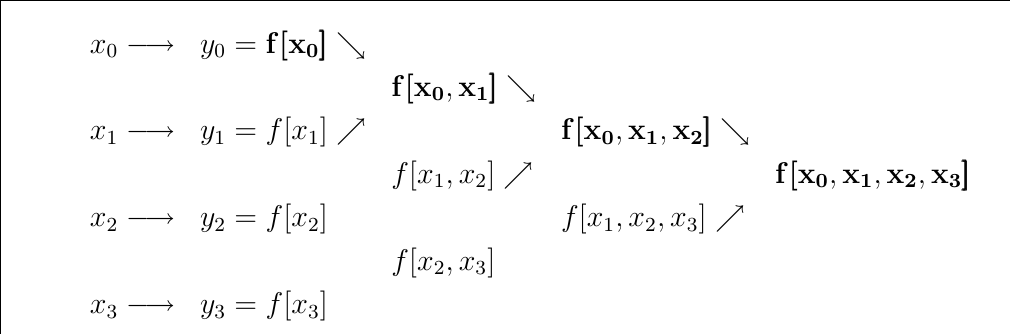
\includegraphics[width=0.9\linewidth]{tema2/diferencias-div}
% \end{center} donde las expresiones situadas en las filas superiores
% (en negritas) coinciden con los coeficientes $\alpha_k$.
% \begin{example} Calcular el polinomio de interpolación de Lagrange
% asociado a la siguiente tabla de datos, haciendo uso de la fórmula de
% las diferencias divididas de Newton:
% \begin{equation*}
%   \begin{array}{grrrcr}
%     \toprule x & 2 & 4 & 6 & 8 & 10 \\
%     \midrule y & 3 & -1 & 4 & 0 & -1 \\ \bottomrule
%   \end{array}
% \end{equation*}
% \end{example}

% Como último comentario en esta sección: la
% expresión~(\ref{eq:pol.newton.dif-div}) de un polinomio $p_n(x)$ da
% pie a una fórmula muy utilizada (por ser poco costosa
% computacionalmente) para la evaluación de el valor de un polinomio en un punto $x=r\in\Rset$. Se trata de la \resaltar{fórmula de Ruffini-Horner}:
% \begin{equation*}
%   p_n(r) = a_0 + (r-x_0)(a_1 + (r-x_1)(a_2 + \cdots + (r-x_n)a_n)\cdots)
% \end{equation*}
% En esta fórmula, el número de multiplicaciones se ve reducida
% sustancialmente con con respecto a la
% expresión~(\ref{eq:pol.newton.dif-div}) .

% % \begin{example}
% %   Utilizaremos la interpolación de $f(x)=2^x$ y la fórmula de
% %   Ruffini-Horner para obtener una aproximación de $\sqrt{2}$.
% % \end{example}

% \subsection{Expresión del error}
% \label{sec:error-interpol-lagrange}
% Como antes, consideremos una función $f(x)$ definida en un intervalo
% $[a,b]$ de la que conocemos los valores $y_i=f(x_i)$ en un soporte
% $\{x_0,x_1,\dots,x_n\}$. El siguiente resultado nos ofrece, suponiendo
% regularidad en $f$, una cota del error de interpolación en cada punto
% de $[a,b]$:
% \begin{theorem}
%   \label{thm:error-interpol-lagrange}
%   Sea $f\in C^{n+1}([a,b])$ y fijemos un soporte de $n+1$ puntos
%   distintos, $S=\{x_0,x_1,\dots,x_n\}\subset[a,b]$. Sea
%   $p_n\in\Pol_n[x]$ el polinomio de interpolación asociado a los valores
%   $y_i=f(x_i)$, $i=0,...,n$. Para cada $x\in[a,b]$, existe $\xi_x\in
%   (a,b)$ tal que:
%   \begin{equation}
%     \label{eq:expresion-error-interpol}
%     f(x)-p_n(x)=\frac{f^{n+1)}(\xi_x)}{(n+1)!} w_S(x),
%   \end{equation}
%   donde $w_S(x)=(x-x_0)(x-x_1)\dots(x-x_n).$
% \end{theorem}

% \begin{proof}
%   Si $x=x_i$ para algún $i=0,...,n$,
%   entonces~(\ref{eq:expresion-error-interpol}) es evidente (ambos
%   miembros de la igualdad se anulan).

%   \etapa{Etapa 1.} Fijemos, en lo que sigue, $x\in[a,b]$ tal que
%   $x\neq x_i$ para todo $i=0,...,n$. Escribiendo
%   \begin{equation}
%     \omega_S(t)=(t-x_0)(t-x_1)\dots (t-x_n),
%     \label{eq:w_S:3}
%   \end{equation}
%   definamos la siguiente función auxiliar:
%   \begin{equation}
%     \phi(t)=f(t)-p_n(t)-\lambda_x\, \omega_S(t), \quad \forall t\in[a,b],
%     \label{eq:interpol:2}
%   \end{equation}
%   donde $\lambda_x$ se calcula de forma que, para el $x$ que hemos
%   fijado, $\phi(x)=0$, es decir,
%   $$
%   \lambda_x = \frac{f(x)-p_n(x)}{\omega_S(x)}.
%   $$
%   Si conseguimos demostrar que existe $\xi_x\in (a,b)$ tal que
%   $\phi^{n+1)}(\xi_x)=0$ hemos terminado, pues derivando $n+1$ veces
%   en~(\ref{eq:interpol:2}) y sustituyendo $t=\xi_x$:
%   \begin{align*}
%     0=\phi^{n+1)}(\xi_x)&=f^{n+1)}(\xi_x)-p_n^{n+1)}(\xi_x)-\lambda_x\cdot\omega_S^{n+1)}(\xi_x)
%     \\
%                         &=f^{n+1)}(\xi_x)- \frac{f(x)-p_n(x)}{\omega_S(x)}\cdot (n+1)!,
%   \end{align*}
%   de donde podemos despejar $f(x)-p_n(x)$ para
%   obtener~(\ref{eq:expresion-error-interpol}) \etapa{Etapa 2.}
%   Utilizando repetidas veces el teorema de Rolle podemos comprobar que
%   existe $\xi_x\in (a,b)$ tal que $\phi^{n+1)}(\xi_x)=0$:

%   Debido a su definición, $\phi$ verifica:
%   $\phi(x_0)=\phi(x_1)=\cdots=\phi(x_n)=0$ y además, por definición de
%   $\lambda_x$, $\phi(x)=0$. Como $\phi\in C^{n+1}([a,b])$ y se anula
%   en $n+2$ puntos distintos, por el Teorema de Rolle tenemos que
%   $\phi'(x)$ se anula en $n+1$ puntos distintos de $(a,b)$. Aplicando
%   sucesivamente el Teorema de Rolle, llegamos a que $\phi^{n+1)}\in
%   C^0([a,b])$ y se anula (al menos) en un punto, $\xi_x\in (a,b)$.
% \end{proof}

% \begin{remark}[Cota uniforme del error]
%   \label{rk:2}
%   El teorema anterior nos proporciona la siguiente cota uniforme del
%   error:
%   \begin{equation}
%     ||f-p_n||_{\infty} \le \frac{M_{n+1}}{(n+1)!}||(x-x_0)\cdots(x-x_n)||_\infty,
%     \label{eq:cota-error-interpol-1}
%   \end{equation}
%   donde para cualquier función $g\in C^0([a,b])$ denotamos
%   \begin{equation*}
%     ||g||_\infty = \max_{x\in[a,b]} |g(x)|  \quad (\text{norma
%       uniforme de $g$})
%   \end{equation*}
%   y $M_{n+1}=||f^{n+1)}||_\infty$.  En particular, se tiene que:
%   \begin{equation*}
%     ||f-p_n||_{\infty} \le \frac{M_{n+1}}{(n+1)!}(b-a)^{n+1}.
%     \label{eq:cota-error-interpol-2}
%   \end{equation*}
% \end{remark}

% \begin{example}
%   \label{ex:expresion-del-error-interpol}
%   Calcular una cota para el error de interpolación de la función
%   $f(x)=\sen(x)$ cuando se toman $4$ puntos en el intervalo $[a,b]=[-\pi/2,\pi/2]$.

%   Como $f^{4)}(x)=\sin(x)$, $M_{n+1}=M_4=\max_{x\in
%     [a,b]}|f^{4)}(x)|\le 1$, y aplicando la
%   acotación~(\ref{eq:cota-error-interpol-1}) para $n=3$ obtenemos:
%   \begin{equation*}
%     ||f-p_4||_\infty \le \frac{1}{4!}(x-x_0)(x-x_1)(x-x_2)(x-x_3).
%   \end{equation*}
%   A partir de ahí podemos concluir que
%   \begin{equation*}
%     ||f-p_4||_\infty \le \frac{1}{4!}(b-a)^4 = \frac{\pi^4}{24}
%     \simeq 4.058
%   \end{equation*}
% \end{example}
% \begin{remark}[Convergencia uniforme de los polinomios de interpolación]
%   Consideremos de nuevo el
%   ejemplo~\ref{ex:expresion-del-error-interpol}. Es fácil ver que, al
%   aumentar el grado del polinomio de interpolación (o equivalentemente
%   el número de nodos del soporte), el error $||f-p_n||_\infty$
%   converge a cero. En efecto, todas las derivadas de $f(x)=\sen(x)$
%   están acotadas por uno, luego
%   \begin{equation*}
%     ||f-p_n||_\infty\le \frac{\pi^n}{(n+1)!} \to 0,
%   \end{equation*}
%   ya que el crecimiento del factorial es más rápido que el de la
%   función exponencial.

%   ¿Ocurre lo mismo con todas las funciones? Es decir, dada una
%   función $f$ suficientemente regular (por ejemplo infinitamente
%   derivable) a la que interpolamos en un soporte de $n+1$ puntos en
%   $[a,b]$,
%   \begin{equation}
%     \text{\Large ¿ \;}
%     \lim_{n\to\infty} p_n(x) = f(x) \quad \forall x\in [a,b]
%     \text{\; \Large?}
%     \label{eq:pregunta.p_n.to.f}
%   \end{equation}
%   Es fácil demostrar (se deja como ejercicio) que $p_n(x)\to f(x)$
%   para todo $x$ de un intervalo cerrado $[a,b]$ si y solo si $||p_n -
%   f||_\infty\to 0$. Por lo tanto, la pregunta anterior es equivalente
%   a:
%   \begin{equation*}
%     \text{\Large ¿ \;}
%     \lim_{n\to\infty} ||f-p_n||_\infty=0
%     \text{\; \Large ?}
%   \end{equation*}
%   La estimación del error de interpolación de
%   Lagrange~(\ref{eq:cota-error-interpol-1}) nos puede dar alguna
%   orientación: para conseguir que
%   $||f-p_n||\to 0$ deberíamos acotar el segundo miembro uniformemente
%   por una sucesión que converge a cero, lo que no es posible en
%   general, pues implica el controlar uniformemente las derivadas
%   $n+1$--ésimas de $f$ en $[a,b]$ cuando $n\to \infty$.

%   Por tanto, la respuesta la pregunta~(\ref{eq:pregunta.p_n.to.f}) es:
%   \textbf{no en general}. Para poderlo asegurar, basta el
%   contraejemplo que se muestra a continuación (una función a la que no
%   converge el polinomio de interpolación de Lagrange en un soporte de
%   puntos equidistantes).
% \end{remark}

% \begin{example}(Fenómeno de Runge)
%   \label{ex:fenomeno-runge}
%   Consideremos en el intervalo $[-1,1]$ la función
%   \begin{equation*}
%     f(x) = \frac{1}{1+25x^2}
%   \end{equation*}
%   junto a un soporte de $n+1$ puntos equiespaciados en $[-1,1]$.
%   \begin{figure}
%     \centering
%     \begin{tabular*}{1.0\linewidth}{cc}
%    \subfloat[$n=2$]{
%     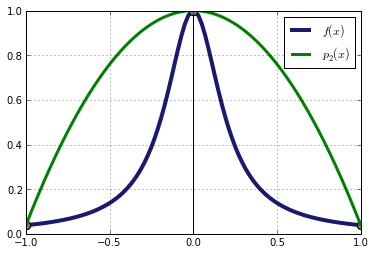
\includegraphics[width=0.45\linewidth]{tema2/runge-n2}} &
%    \subfloat[$n=4$]{
%     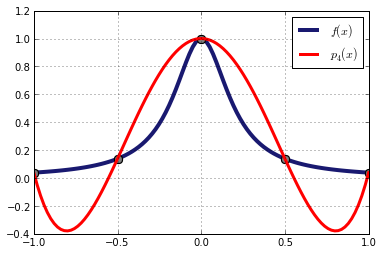
\includegraphics[width=0.45\linewidth]{tema2/runge-n4}}
%       \\
%    \subfloat[$n=6$]{
%     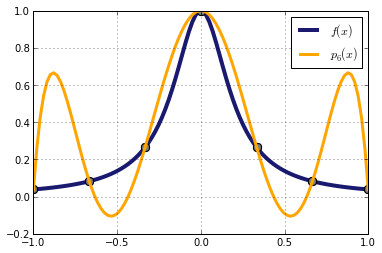
\includegraphics[width=0.45\linewidth]{tema2/runge-n6}} &
%    \subfloat[$n=8$]{
%     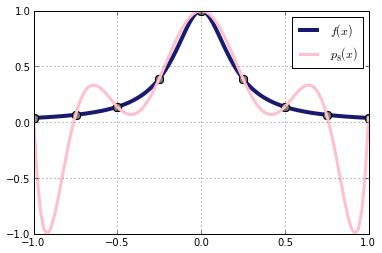
\includegraphics[width=0.45\linewidth]{tema2/runge-n8}}
%     \end{tabular*}
%     \caption{Fenómeno de Runge: interpolación de la función
%       $f(x)=1/(1+25x^2)$ (en color azul) mediante polinomios de
%       lagrange $p_n(x)$ con $n=2,4,6,8$}.
%     \label{fig:fenomeno-runge}
%   \end{figure}
%   Si representamos gráficamente el polinomio de interpolación de
%   Lagrange, $p_n(x)$ (figura~\ref{fig:fenomeno-runge}), veremos que a
%   medida que $n$ crece se producen grandes oscilaciones cerca de los
%   extremos del intervalo.
% \end{example}


% La observación anterior es importante, pues significa que \textbf{no siempre
%   podemos conseguir mejorar la aproximación de una función mediante el
%   incremento del grado del polinomio de interpolación de Lagrange}.
% Obsérvese que este hecho no entra en contradicción con el teorema de
% aproximación de Weierstrass (que afirma que los polinomios son densos
% en las funciones continuas con la norma uniforme). Simplemente: no
% siempre el interpolador de Lagrange es la mejor aproximación por
% polinomios de una función continua.

% Para mitigar este problema existen distintas posibilidades como:
% \begin{enumerate}
% \item Escoger cuidadosamente el soporte de interpolación.
% \item Utilizar interpolación a trozos (en particular, interpolación mediante funciones ``\textit{spline}'' o ``ranura'').
% \item Renunciar a la interpolación y utilizar otro tipo de técnica
%   para la aproximación, como mínimos cuadrados.
% \end{enumerate}

% En la siguiente sección, estudiaremos la segunda de estas
% posibilidades.

% \section{Interpolación a trozos. Funciones \textit{spline} o ranura}
% \label{sec:interp-trozos-splines}

% \subsection{Interpolacion a trozos}
% \label{sec:interpolacion-trozos}


% Dada una función $f$ continua en $[a,b]$, la idea de la interpolación
% a trozos consiste en fijar una partición ${\cal
%   P}=\{a=x_0<x_1<\cdots<x_n=b\}$ para aproximar a $f$ mediante
% interpolación de Lagrange en cada uno de los subintervalos
% $[x_{i-1},x_{i}]$, $i=1,...,n$, de modo que el grado de estos
% polinomios, $m$, sea pequeño (en la práctica $m=1$, $2$ ó $3$) y la
% función resultante sea continua entre estos subintervalos.

% Definamos el diámetro de la partición como
% $h=\max_{i\in\{1,...,n\}}(x_i-x_{i-1})$. Nuestro propósito es aumentar
% el número de subintervalos (es decir hacer $n\to \infty$) de forma
% que $h\to 0$, mientras mantenemos constante el grado de los polinomios
% de interpolación.

% Más específicamente, definimos el conjunto de las \resaltar{funciones
%   continuas y polinómicas a trozos} como:
% \begin{equation*}
%   V_h = \{ q_h\in C^0([a,b]) \ /\ q_h|_{[x_{i-1},x_{i}]}\in \Pol_m[x]\
%   \forall i=1,...,n \}.
% \end{equation*}
% Para cada $i=1,...,n$, consideramos el subintervalo $[x_{i-1},x_i]$ y
% definimos $m-1$ nodos interiores, $\xi_{ij}\in (x_{i-1},x_i)$ (con
% $j=1,\dots,m-1$). Para los datos anteriores, definimos la
% \resaltar{función de interpolación polinómica a trozos}, $p_h$, como
% la única función de $V_h$ que en cada intervalo $[x_{i-1},x_i]$
% interpola los valores de $f$ en los $m+1$ nodos situados en $[x_{i-1},
% x_{i}]$.  Es decir, para cada $i=1,\dots n$:
% \begin{align*}
%   p_h(x_{i-1})&=f(x_{i-1}),\\
%   p_h(\xi_{ij})&=f(\xi_{ij}), \quad j=1,...,m-1,\\
%   p_h(x_i)&=f(x_i).
% \end{align*}

% \begin{theorem}[Estimación de error]
%   \label{thm:interpol-trozos-error}
%   Si $f\in C^{m+1}( [a,b])$ y $p_h$ es el interpolador a trozos
%   definido anteriormente:
%   \begin{equation}
%     ||f-p_h||_\infty\le\frac{M_{m+1}}{(m+1)!}h^{m+1},
%     \quad
%     \text{ donde } M_{m+1}=||f^{m+1)}||_\infty.
%     \label{eq:interpol-trozos-error}
%   \end{equation}
% \end{theorem}

% \begin{proof}
%   Consideremos $||f-p_h||_{\infty, [a,b]}=\max\{ |f(x)-p_h(x)|\ /\
%   x\in[a,b]\}$.
%   \begin{itemize}
%   \item Este máximo se alcanza en algún subintervalo $[x_{i-1},x_{i}]$
%     es decir $||f-p_h||_{\infty}=||f-p_h||_{\infty, [x_{i-1},x_i]}$
%     para algún $i=1,\dots,n$.
%   \item En este subintervalo podemos usar el
%     teorema~\ref{thm:error-interpol-lagrange}, por lo que
%     \begin{align*}
%       ||f-p_h||_\infty &= ||f-p_h||_{\infty, [x_{i-1},x_i]}  \\
%                        &\le\frac{M_{m+1}}{(m+1)!}
%                          (x-x_{i-1})(x-\xi_{i1})\cdots(x-\xi_{i,m-1})(x-x_i).
%     \end{align*}
%   \end{itemize}
%   Como cada uno de estos factores es menor que $h$, finaliza la
%   demostración.
% \end{proof}

% \begin{remark}
%   \label{rk:3}
%   En el caso de interpolación a trozos, podemos garantizar que, si
%   $f\in C^{m+1}([a,b])$,
%   \begin{equation*}
%     ||f-p_h||_\infty \to 0 \quad \text{cuando } h \to 0,
%   \end{equation*}
%   pues el término $M_{m+1}/(m+1)!$ permanece constante
%   en~\ref{eq:interpol-trozos-error} cuando $h\to 0$.
% \end{remark}

% \subsection{Interpolación por funciones \textit{spline} o ranura}
% \label{sec:splines}

% Nos centraremos ahora en
% el caso en que se aumenta la regularidad del interpolante.
% Es decir, dada una partición
% ${\cal P}= \{a = x_0 <x_1 < \cdots <x_n=b\}$
% del intervalo $[a,b]$ y dados unos datos $y_0$, $y_1$, \dots, $y_n$
% (que eventualmente podrían venir dados como $y_i=f(x_i)$ para alguna
% función $f$), nos proponemos el construir:
% \begin{itemize}
% \item  funciones polinómicas a trozos, en los subintervalos que
%   denotaremos $I_i=[x_{i},x_{i+1}]$ (para $ i=0,\dots,n-1$)
% \item que interpolen los valores $\{y_i\}_{i=0}^n$ en el soporte
%   $S=\{x_i\}_{i=0}^n$ y
% \item que sean <<regulares>> en $[a,b]$.
% \end{itemize}
% En la práctica, se utiliza regularidad $C^{k-1}([a,b])$, donde
% $k\in\Nset$ es el grado de los polinomios de
% interpolación en los subintervalos $I_i$. Concretamente:
% % , en lo que sigue nos centraremos en el conjunto:
% % \begin{equation*}
% %   V_h = \{q_h \in C^{k-1}([a,b])\ / \ q_h|_{I_i}}\in
% %   \Pol_k[x],\ \forall i=0,\dots,n-1\},
% % \end{equation*}
% % donde denotamos $I_i=[x_{i+1},x_i]$ para $ i=0,\dots,n-1$.

% \begin{definition}[Funciones spline o ranura]
%   \label{def:funcion-spline}
%   Sea una partición ${\cal P}= \{a = x_0 <x_1 < \cdots <x_n=b\}$ del
%   intervalo $[a,b]$ y unos valores $\{y_i\}_{i=0}^n$. Fijado
%   $k\in\Nset$, consideremos el espacio de las funciones que son
%   de clase $C^{k-1}$ en $[a,b]$ y que en cada subintervalo son
%   polinomios de grado $k$:
%   \begin{equation*}
%     V_h = \{q_h \in C^{k-1}([a,b])\ / \ q_h|_{I_i}\in  \Pol_k[x],\ \forall i=0,\dots,n-1\}.
%   \end{equation*}
%   Llamamos función \resaltar{spline} (o \resaltar{ranura}) a
%   cualquier $s_h\in V_h$. Decimos que una función spline $s_h\in V_h$
%   interpola los datos $\{(x_i,y_i)\}_{i=0}^n$ si $s_h(x_i)=y_i$ para
%   todo $i=0,\dots,n$.
% \end{definition}

% Al caso $k=1$ se le llama \textit{spline lineal} y coincide (para
% polinomios de dimensión uno) con la interpolación a trozos estudiada
% en el apartado anterior Al caso $k=2$ se le llama \textit{spline
%   cuadrático} y a $k=3$, \textit{spline cúbico}. Splines lineales y
% cúbicos son los más utilizados en la práctica.

% \subsubsection{Splines lineales}
% \label{sec:splines-lineales}

% Consideremos
% \begin{equation*}
%   V_h = \{q_h \in C^{0}([a,b])\ / \ q_h|_{I_i}\in  \Pol_1[x],\ \forall i=0,\dots,n-1\}.
% \end{equation*}
% Una función $s_h\in V_h$ que interpole los datos
% $\{(x_i,y_i)\}_{i=0}^n$ queda determinada por las siguientes $n$
% ecuaciones (que resultan de escribir, en cada subintervalo $I_i=[x_i,
% x_{i+1}]$, la ecuación de la recta que pasa por los puntos
% $(x_i,y_i)$ y $(x_{i+1},y_{i+1})$):
% \begin{equation*}
%   \label{eq:splines-lineales-1}
%   s_h(x) = l_i(x) = y_i + \frac{y_{i+1}-y_i}{x_{i+1}-x_i}(x-x_i) \quad
%   \forall x\in I_i.
% \end{equation*}

% \begin{example}
%   \label{ex:splines-lineales-1}
%   Interpolar, mediante splines lineales, los siguientes
%   datos:
%   \begin{equation*}
%     \{ (1,2),\ (2,-1),\ (3,0),\ (4,1) \},
%   \end{equation*}
% \end{example}
% es decir:
% \begin{equation}
%   \small
%   \begin{array}{r@{\rule{4ex}{0pt}}rrrcr}
%     % \toprule
%     i & 0 & 1 & 2 & 3
%     \\ \toprule %\cline{1-5}
%     x_i & 1 & 2 & 3 & 4
%     \\ \midrule
%     y_i & 2 & -1 & 0  & 1
%     \\
%     \bottomrule
%   \end{array}
%   \label{eq:tabla-datos-lagrange-splines}
% \end{equation}
% Escribiendo las ecuaciones anteriores para estos datos obtenemos:
% \begin{equation*}
%   s_h(x)=\left\{
%     \begin{tabular}{rll}
%       $2 -3 (x-1)$ & si & $x\in[1,2]$,
%       \\\noalign{\medskip}
%       $-1 + (x-2)$ & si & $x\in[2,3]$
%       \\\noalign{\medskip}
%       $0 - (x-3)$ & si & $x\in[3,4]$
%     \end{tabular} \right.
%   \quad=\qquad
%   \left\{
%     \begin{tabular}{rll}
%       $5 -3x$ & si & $x\in[1,2]$,
%       \\\noalign{\smallskip}
%       $x-3$ & si & $x\in[2,3]$,
%       \\\noalign{\smallskip}
%       $x-3$ & si & $x\in[3,4]$.
%     \end{tabular} \right.
% \end{equation*}

%    \subsubsection{Splines cúbicos}
%    \label{sec:splines-lineales}

%    Consideremos ahora el espacio
%    \begin{equation*} V_h = \{q_h \in C^{2}([a,b])\ / \ q_h|_{I_i}\in
%      \Pol_3[x],\ \forall i=0,\dots,n-1\}.
%    \end{equation*} Nos proponemos calcular una función $s_h\in V_h$ (un
%    spline cúbico) que interpole unos datos determinados,
%    $\{(x_i,y_i)\}_{i=0}^n$. Comprobaremos que este problema es
%    equivalente a un sistema de ecuaciones lineales.

%    En cada intervalo $I_i=[x_i, x_{i+1}]$, el spline cúbico es un
%    polinomio de grado tres, es decir, para cada $i=0,\dots,n-1$ se tiene:
%    \begin{equation}
%      s_h(x) = s_i(x) = a_i + b_ix + c_ix^2 + d_ix^3,\quad
%      \forall x\in I_i.
%      \label{eq:spline-cubico}
%    \end{equation}
%    Para calcular el spline $s_h$ es necesario determinar $\{a_i, b_i,
%    c_i, d_i\}_{i=0}^{n-1}$, es decir $4n$ incógnitas. Por lo tanto,
%    necesitaremos $4n$ ecuaciones, que se obtienen de la siguiente forma:
%    \begin{itemize}
%    \item $n+1$ condiciones provienen de la interpolación de los datos
%      $\{(x_i, y_i)\}_{i=0}^n$:
%      $$
%      s_i(x_i)=y_i, \quad i=0,1,\dots,n.
%      $$
%    \item $3(n-1)$ condiciones provienen  de la regularidad de $s_h$ en
%      $[a,b]$. En concreto:
%      \begin{equation*}
%        \left.
%          \begin{aligned}
%            s_{i-1}(x_i)&=s_{i}(x_i) \quad \text{(continuidad de $s_h$)}
%            \\
%            s'_{i-1}(x_i)&=s'_{i}(x_i) \quad \text{(continuidad de $s_h'$)}
%            \\
%            s''_{i-1}(x_i)&=s''_{i}(x_i) \quad \text{(continuidad de $s_h''$)}
%          \end{aligned}
%        \right\} \quad \forall i=1,\dots,n-1
%      \end{equation*}
%    \item Sumando, tenemos $(n+1) + 3(n-1) = 4n-2$ ecuaciones, para las
%      $4n$ incógnitas de las que partimos. Necesitamos $2$ ecuaciones
%      más, que se suelen imponer sobre los extremos del intervalo
%      $[a,b]$. Las más utilizadas son:
%      \begin{itemize}
%      \item Si disponemos de información sobre la derivada en los
%        extremos, $y_a'$, $y_b'\in\Rset$, imponemos:
%        \begin{equation*}
%          s_0'(a)=y_a', \quad s_n'(b)=y_b' \quad \text{(condición de frontera fija)}.
%        \end{equation*}
%      \item Si carecemos de la información anterior, suele imponerse que
%        la segunda derivada se anule en los extremos:
%        \begin{equation*}
%          s_0''(a)=0, \quad s_n''(b)=0 \quad \text{(condición natural o de
%          frontera libre)}.
%        \end{equation*}
%      \end{itemize}
%    \end{itemize}

%    \begin{example}
%      \label{ex:splines-cubicos}
%      \begin{figure}
%        \centering
%        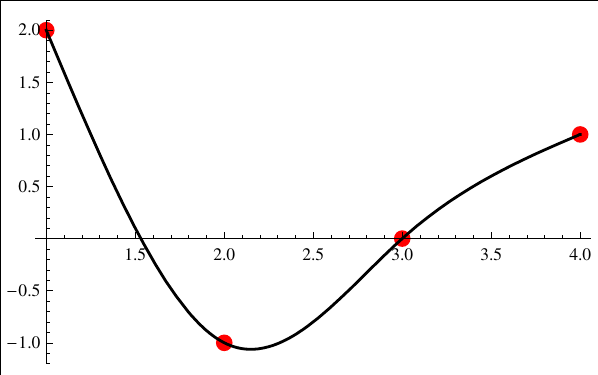
\includegraphics[width=0.4\linewidth]{tema2/spline-cubico}
%        \caption{Spline cúbico que interpola los puntos de la
%          tabla~\ref{eq:tabla-datos-lagrange-splines}.}
%        \label{fig:spline-cubico}
%      \end{figure}
%      A continuación plantearemos el sistema de ecuaciones que resulta al
%      usar splines cúbicos naturales para
%      interpolar los datos del ejemplo~\ref{ex:splines-lineales-1}. Para
%      ello, reescribimos~(\ref{eq:spline-cubico}) como:
%      \begin{equation*}
%        s_h(x)=\left\{
%          \begin{aligned}
%            s_0(x)&=a_0 + b_0(x-1) + c_0(x-1)^2 + d_0(x-1)^3
%            & \text{si} && x\in[1,2],
%            \\
%            s_1(x)&=a_1 + b_1(x-2) + c_1(x-2)^2 + d_1(x-2)^3
%            &\text{si}&& x\in[2,3],
%            \\
%            s_2(x)&=a_2 + b_2(x-3) + c_2(x-3)^2 + d_2(x-3)^3
%            & \text{si}&& x\in[3,4].
%          \end{aligned}\right.
%      \end{equation*}
%    \end{example}

%    Tenemos $12$ incógnitas y disponemos de las siguientes ecuaciones:
%    \begin{enumerate}
%    \item Interpolación:
%      \begin{itemize}
%      \item Imponiendo $s_h(x_i)=y_i$, $i=0,1,2$, llegamos directamente
%        a
%        \begin{equation*}
%          a_0=2, \quad a_1=-1, \quad a_2=0
%        \end{equation*}
%      \item Imponiendo $s_h(x_3)=s_2(x_3)=y_3$, llegamos a:
%        \begin{equation*}
%          a_2+b_2+c_2+d_2=1.
%        \end{equation*}
%      \end{itemize}
%    \item Continuidad:
%      \begin{align*}
%        s_0(x_1)=s_1(x_1) &\Rightarrow a_0+b_0+c_0+d_0 = a_1,
%        \\
%        s_1(x_2)=s_2(x_2) &\Rightarrow a_1+b_1+c_1+d_1 = a_2.
%      \end{align*}
%    \item Continuidad de $s_h'$. Usando que
%      $s_i'(x)=b_i+2c_i(x-x_i)+3d_i(x-x_i)^2$:
%      \begin{align*}
%        s_0'(x_1)=s_1'(x_1) &\Rightarrow b_0+2c_0+3d_0 = b_1,
%        \\
%        s_1'(x_2)=s_2'(x_2) &\Rightarrow b_1+2c_1+3d_1 = b_2.
%      \end{align*}
%    \item Continuidad de $s_h''$. Usando que
%      $s_i'(x)=2c_i+6d_i(x-x_i)$:
%      \begin{align*}
%        s_0''(x_1)=s_1''(x_1) &\Rightarrow 2c_0+6d_0 = 2c_1,
%        \\
%        s_1''(x_2)=s_2''(x_2) &\Rightarrow 2c_1+6d_1 = 2c_2.
%      \end{align*}
%    \item Además imponemos condiciones naturales en $x_0$ y en $x_3$, es decir
%      $s_0''(x_0)=0$, $s_2''(x_3)=0$, de donde:
%      \begin{equation*}
%        2c_0 = 0, \quad 2c_2 + 6 d_2 =0.
%      \end{equation*}
%    \end{enumerate}

%    En notación matricial, tenemos el siguiente sistema de ecuaciones:
%    \newcommand{\z}{\color{gray}0}
%    \begin{equation*}
%      \left[
%        \begin{array}{rrrr@{\rule{1.3em}{0pt}}rrrr@{\rule{1.3em}{0pt}}rrrr}
%          1&\z&\z&\z& \z&\z&\z&\z& \z&\z&\z&\z \\
%          \z&\z&\z&\z& 1&\z&\z&\z& \z&\z&\z&\z \\
%          \z&\z&\z&\z& \z&\z&\z&\z& 1&\z&\z&\z \\
%          \z&\z&\z&\z& \z&\z&\z&\z& 1&1&1&1 \\\noalign{\medskip}

%          1&1&1&1& -1&\z&\z&\z& \z&\z&\z&\z \\
%          \z&\z&\z&\z& 1&1&1&1& -1&\z&\z&\z \\
%          \z&1&2&3& \z&-1&\z&\z& \z&\z&\z&\z \\
%          \z&\z&\z&\z& \z&1&2&3& \z&-1&\z&\z \\\noalign{\medskip}

%          \z&\z&2&6& \z&\z&-2&\z& \z&\z&\z&\z \\
%          \z&\z&\z&\z& \z&\z&2&6& \z&\z&-2&\z \\
%          \z&\z&2&\z& \z&\z&\z&\z& \z&\z&\z&\z \\
%          \z&\z&\z&\z& \z&\z&\z&\z& \z&\z&2&6 \\
%        \end{array}
%      \right]
%      \
%      \left[
%        \begin{array}{r}
%          a_0 \\ b_0 \\ c_0 \\ d_0 \\ \noalign{\medskip}
%          a_1 \\ b_1 \\ c_1 \\ d_1 \\ \noalign{\medskip}
%          a_2 \\ b_2 \\ c_2 \\ d_2
%        \end{array}
%      \right]
%      =
%      \left[
%        \begin{array}{r}
%          2 \\ -1 \\ 0 \\ 1 \\ \noalign{\medskip}
%          \z \\  \z \\ \z \\ \z \\ \noalign{\medskip}
%          \z \\  \z \\ \z \\ \z
%        \end{array}
%      \right]
%    \end{equation*}
%    Se puede demostrar (ver [Burden \& Faires] en la bibliografía) que
%    este los sistemas de ecuaciones que aparecen en interpolación
%    mediante splines tienen una única solución y que (como en el caso de
%    splines lineales) los splines cúbicos convergen a la función
%    interpolada, siempre que ésta sea suficientemente regular. Aunque
%    en el sistema anterior se pueden eliminar fácilmente algunas
%    incógnitas ($a_0$, $a_1$, $a_2$ y $c_0$), el sistema resultante es
%    de orden $8\times 8$ y en la práctica debe ser resuelto mediante el
%    ordenador (especialmente cuando  aumente el número de
%    subintervalos). Como resultado, se obtienen los coeficientes de los
%    polinomios de grado $3$ en $[1,2]$, $[2,3]$ y $[3,4]$ que definen
%    el spline cúbico. Estos polinomios han sido representados en la
%    figura~\ref{fig:spline-cubico}.


%    % \subsubsection*{En resumen}
%    En resumen, en esta sección hemos conseguido mitigar el problema de
%    convergencia que puede presenta la interpolación de datos cuando
%    aumenta el grado de los polinomios. Para ello se han utilizado de
%    funciones polinómicas a trozos y regulares en $[a,b]$, para las que
%    hemos probado convergencia uniforme en el caso $C^0([a,b])$. Como
%    ejemplo final, se presentan dos imágenes (extraídas de [Burden \&
%    Faires]): en la a figura~\ref{fig:pato-alto-orden} se utiliza un
%    polinomio de alto orden, generándose grandes oscilaciones. En la
%    figura~\ref{fig:pato-spline} se utilizan funciones splines cúbicas,
%    obteniéndose excelentes resultados.


%   \begin{figure}
%     \begin{center}
%       \begin{tabular}{c}
%         \subfloat[Interpolación con polinomios de alto orden]{
%         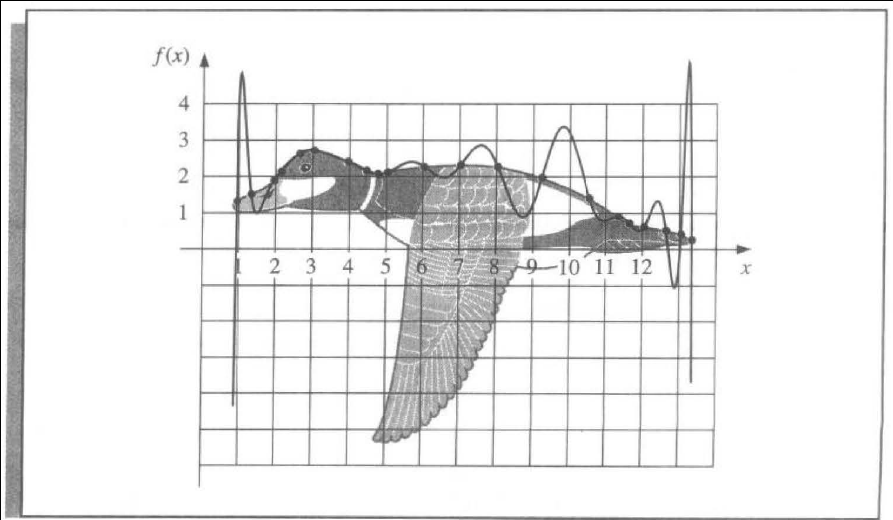
\includegraphics[width=0.8\linewidth]{tema2/pato-interpol}
%         \label{fig:pato-alto-orden}
%         } \\[1em]
%         \subfloat[Interpolación con splines cúbicos]{
%         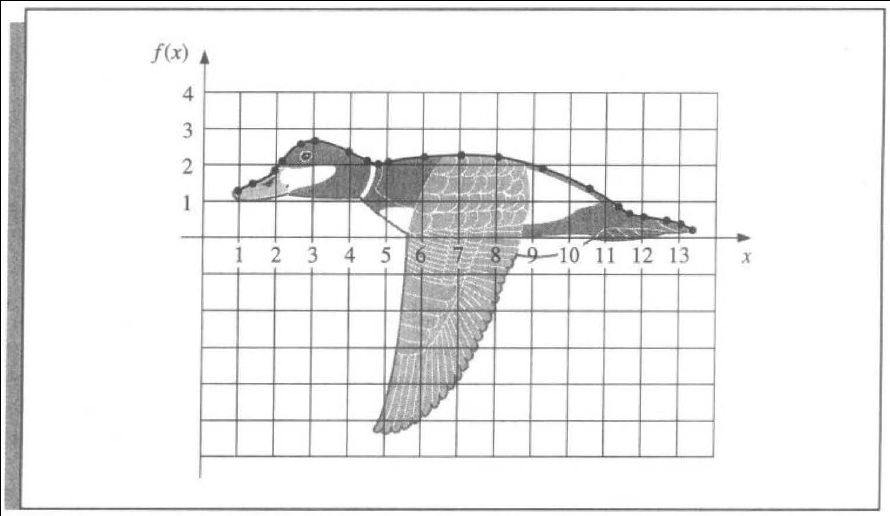
\includegraphics[width=0.8\linewidth]{tema2/pato-spline}
%         \label{fig:pato-spline}}
%       \end{tabular}
%     \end{center}
%   \end{figure}


% \section{Interpolación de Hermite}
% \label{sec:interp-de-hermite}

% Consideremos ahora un conjunto de datos definido por un soporte de
% $n+1$ nodos distintos, $S=\{x_0,x_1,\dots,x_n\}\subset \Rset$ junto al
% siguiente conjunto de $2(n+1)$ datos:
% \begin{equation}
%   \{y_0,y_1\dots,y_n\} \cup \{y'_0,y'_1\dots,y'_n\}.
%   \label{eq:datos-hermite}
% \end{equation}
% Habitualmente, estos datos vienen dados por valores conocidos
% de una función derivable, en concreto  $y_i=f(x_i)$ e
% $y'_i=f'(x_i)$ para alguna función $f$.

% Se trata de encontrar un polinomio $p(x)$ del menor grado posible tal
% que
% \begin{equation}
%   \left.
%     \begin{aligned}
%       p(x_i) &= y_i \\ p'(x_i)&=y_i'
%     \end{aligned}
%   \right\}\quad \forall i=0,\dots,n.
%   \label{eq:interpolacion-hermite}
% \end{equation}
% Un polinomio con estas características se llama polinomio de
% interpolación de Hermite.

% \subsection{Existencia y unicidad}
% \label{sec:exist-y-unic}

% \begin{theorem}[Existencia y unicidad]
%   Dado un soporte de $n+1$ nodos distintos, $x_0$,
%   $x_1$,\dots,$x_n\in\Rset$ y dados $2n+2$ datos como
%   en~(\ref{eq:datos-hermite}), existe un único polinomio de grado
%   $2n+1$ que interpola estos datos, en el sentido
%   de~(\ref{eq:interpolacion-hermite}).
% \end{theorem}

% \subsection*{Construcción del polinomio de interpolación de Hermite}
% \label{sec:constr-del-polin-hermite}

% Es posible comprobar que el polinomio de hermite que interpola los
% datos~(\ref{eq:datos-hermite}) en un soporte $\{x_0,\dots,x_n\}$
% viene dado por:
% \begin{equation*}
%   p(x)=\sum_{i=0}^{2n+1}(u_i(x)y_i+ v_i(x)y'_i),
% \end{equation*}
% donde
% \begin{align*}
%   u_i(x)&=\left[1-2L'_i(x_i)(x-x_i)\right]\, L_i^2(x)
%   \\ \noalign{\smallskip}
%   v_i(x)&=(x-x_i)\, L_i^2(x),
% \end{align*}
% siendo $\{L_i\}_{i=0}^n$ la base de Lagrange asociada al soporte,
% es decir, cada $L_i$ es el único polinomio de grado $n$ tal que:
% \begin{equation}
%   L_i(x_j)= \delta_{ij} =
%   \left\{\begin{array}{l}
%            1 \text{ si } i=j, \\\noalign{\medskip} 0 \text{ si } i\neq j
%          \end{array}\right.
%      \end{equation}

%      El inconveniente de esta formulación del polinomio de interpolación de
%      Hermite es que es computacionalmente costosa cuando el número de nodos
%      es relativamente alto. En la práctica, suele ser más eficiente el
%      utilizar la siguiente alternativa, basada en el uso de diferencias
%      divididas:


%      \begin{theorem}
%        \label{thm:formula-newton-hermite}
%        Sea $f:[a,b]\to\Rset$ derivable y sea $\{x_i\}_{i=0}^n$ un soporte
%        de $n+1$ nodos distintos y ordenados, esto es,
%        $x_0<x_1<\cdots<x_n$. Denotemos $z_{2i}=x_i$ y $z_{2i+1}=x_i$, esto es:
%        \begin{alignat*}{2} % 2 rl columns
%          z_0&=x_0, & z_1&=x_0,\\
%          z_2&=x_1, & z_3&=x_1,\\
%          &\ \vdots & &\ \vdots \\
%          z_{2n}&=x_n, \qquad & z_{2n+1}&=x_n.
%        \end{alignat*}
%        Entonces, el polinomio de Hermite puede construirse como:
%        \begin{equation*}
%          p_{2n+1}(x)=\sum_{i=0}^{2n+1}f[z_0,\dots,z_i]
%          (x-z_0)(x-z_1)\cdots(x-z_{i-1}),
%        \end{equation*}
%        donde $f[z_0,...,z_i]$ son las diferencias divididas estudiadas
%        anteriormente con la siguiente excepción: si
%        $z_i=z_{i+1}$, se define $f[z_i,z_{i+1}]=f'(z_i)$.
%      \end{theorem}

%      \subsection*{Expresión del error}
%      \label{sec:expresion-del-error-hermite}

%      Para la interpolación de Hermite se tiene una expresión del error
%      similar a la obtenida en el teorema~\ref{thm:error-interpol-lagrange}:
%      \begin{theorem}
%        Sea $f\in C^{2n+2}([a,b])$ y sea $p_{2n+1}(x)$ el polinomio de
%        Hermite asociado a los datos $y_i=f(x_i)$, $y'_i=f'(x_i)$ en un
%        soporte $\{x_i\}_{i=0}^n$. Entonces, para cada $x\in [a,b]$ existe
%        $\xi_x\in (a,b)$ tal que:
%        \begin{equation*}
%          % \label{eq:expresion-error-interpol-hermite}
%          f(x)-p_{2n+1}(x)=\frac{f^{2n+2)}(\xi_x)}{(2n+2)!} (x-x_0)^2(x-x_1)^2\dots(x-x_n)^2.
%        \end{equation*}
%      \end{theorem}

% \section{Aproximación mediante mínimos cuadrados}
% \label{sec:minimos-cuadrados}

% \begin{quotation}
%   \it\tiny El día de Año Nuevo de 1801, el astrónomo italiano Giuseppe
%   Piazzi descubrió el planeta enano Ceres. Fue capaz de seguir su
%   órbita durante 40 días. Durante el curso de ese año, muchos
%   científicos intentaron estimar su trayectoria con base en las
%   observaciones de Piazzi (resolver las ecuaciones no lineales de
%   Kepler es muy difícil). La mayoría de las evaluaciones
%   fueron inútiles; el único cálculo suficientemente preciso para
%   permitir a Franz Xaver von Zach, astrónomo alemán, reencontrar a
%   Ceres al final del año fue el de Carl Friedrich Gauss, por entonces
%   un joven de 24 años (los fundamentos de su enfoque ya los había
%   planteado en 1795, cuando aún tenía 18 años). Sin embargo, su método
%   de mínimos cuadrados no se publicó sino hasta 1809, y apareció en el
%   segundo volumen de su trabajo sobre mecánica celeste, Theoria Motus
%   Corporum Coelestium in sectionibus conicis solem ambientium. El
%   francés Adrien-Marie Legendre desarrolló el mismo método de forma
%   independiente en 1805.  En 1829, Gauss fue capaz de establecer la
%   razón del éxito maravilloso de este procedimiento: simplemente, el
%   método de mínimos cuadrados es óptimo en muchos aspectos. El
%   argumento concreto se conoce como teorema de Gauss-Márkov.
%   \par\hfill
%   -- Wikipedia. Último acceso: 7/4/2014.
% \end{quotation}

% Con frecuencia en entornos científicos, la relación entre dos
% variables es solamente conocida como resultados de medidas
% experimentales, de datos estadísticos, etc. Por tanto, los datos están
% sujetos a errores y no tiene sentido el plantear que interpolen
% exactamente una serie de valores. En vez de ello nos planteamos el
% siguiente problema:

% Dados una serie de datos
% \begin{equation}
%   \{(x_0,y_0),(x_1,y_1),\dots,(x_n,y_n)\},
%   \label{eq:datos-min-cuadrados}
% \end{equation}
% determinar una función, $g(x)$, que sea ``fácil de calcular'' y tal
% que, el error $|y_i-g(x_i)|$ ``sea mínimo'' en un sentido a precisar.

% Este problema se puede generalizar en el siguiente sentido: dado un espacio
% vectorial normado $(V,||\cdot||)$ y dado $U\subset V$, para cada $f\in
% V$ decimos que $\overline u$ es \textit{la mejor aproximación} a $f$
% en $U$ si se verifica:
% \begin{equation*}
%   ||f-\overline u|| \le ||f-u||, \quad \forall u\in U.
% \end{equation*}
% Por falta de espacio, no abordaremos el estudio del problema de la
% mejor aproximación y nos centraremos en el caso de la
% aproximación mediante mínimos cuadrados lineales.

% En concreto, dados los datos~(\ref{eq:datos-min-cuadrados}), nos
% proponemos hallar una función afín (una recta)
% \begin{equation}
%   g(x)=ax+b, \quad a,b\in\Rset,\label{eq:5}
% \end{equation}
% tal que
% \begin{equation*}
%   m(a,b) := \sum_{i=0}^n
%   \left(
%     y_i - g(x_i)
%   \right)^2
%   =
%   \left(
%     y_i - a x_i - b
%   \right)^2
% \end{equation*}
% sea mínimo (figura~\ref{fig:min-cuadrados-lineales}).

% \begin{figure}
%   \centering
%   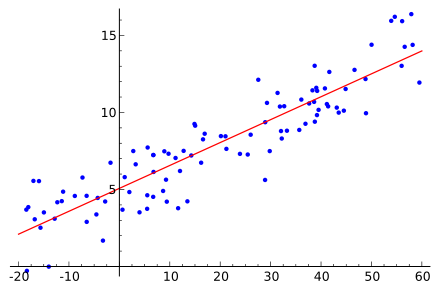
\includegraphics[width=0.6\linewidth]{tema2/linear_regression}
%   \caption{Mínimos cuadrados lineales}
%   \label{fig:min-cuadrados-lineales}
% \end{figure}

% Para ello:
% \begin{align*}
%   \frac{\partial m}{\partial a} & =
%                                   -2\sum_{i=0}^n
%                                   x_i\left(
%                                   y_i - a x_i - b
%                                   \right) =
%                                   -2\sum_{i=0}^n x_i y_i
%                                   +2a\sum_{i=0}^n x_i^2
%                                   +2b\sum_{i=0}^n x_i
%                                   = 0
%                                   \quad \text{y} \\
%   \frac{\partial m}{\partial b} & =
%                                   -2\sum_{i=0}^n
%                                   \left(
%                                   y_i - a x_i - b
%                                   \right) =
%                                   -2\sum_{i=0}^n  y_i
%                                   +2a\sum_{i=0}^n x_i
%                                   +2nb
%                                   = 0.
% \end{align*}

% Basta resolver este sistema lineal de ecuaciones con incógnitas $a$ y
% $b$ para obtener la recta~(\ref{eq:5}) que buscamos:
% \begin{center}
%   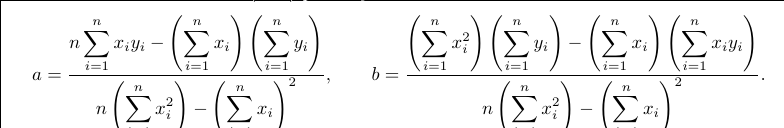
\includegraphics[width=0.9\linewidth]{tema2/ecuacion-min-cuadr}
% \end{center}

% La idea anterior es generalizable a otro tipo de funciones, $g(x)$,
% por ejemplo funciones cuadráticas (aproximación mediante polinomios de
% grado dos).  En prácticas de ordenador veremos algunos ejemplos de
% aproximación mediante mínimos cuadrados.

% \begin{EjerciciosPropuestos}
%   \begin{problema}
%     Consideremos la función $f(x)=\sin(x)$ y su polinomio de
%     interpolación de Lagrange, $p_n(x)$, en el soporte de puntos
%     $S=\{x_k\}_{k=0}^n= \{\pi\,(k+1)/2\}_{i=0}^n$.
%     \begin{enumerate}
%     \item Utilizando la fórmula de diferencias divididas de Newton,
%       calcular $p_3(x)$.
%     \item Argumentar si podemos esperar que se verifique
%       $$
%       \lim_{n\to\infty} p_n(0) = f(0).
%       $$
%       \begin{quote}\em\small
%       Indicación: la expresión del error de interpolación de Lagrange es:<
%       \begin{equation*}
%         f(x)-p_n(x)=\frac{f^{n+1)}(\xi_x)}{(n+1)!}
%         (x-x_0)(x-x_1)\dots(x-x_n), \quad\text{con } \xi\in (a,b).
%       \end{equation*}
%     \end{quote}
%   \end{enumerate}
% \end{problema}

% \begin{problema}
%     Para cada $n\in\Nset$ se considera el soporte definido por $n+1$
%     puntos equiespaciados, $S_{n+1}=\{x_0,x_1,...,x_n\}$, en el intervalo
%     $[-1,1]$.  Calcular una cota para el error cometido al aproximar
%     las siguientes funciones mediante el polinomio de interpolación
%     de Hermite, $p_{2n+1}$, en $S_{n+1}$. Analizar, en cada caso, su
%     convergencia cuando $n\to\infty$.
%     \begin{itemize}
%     \item $\displaystyle f_1(x)=\cos x$
%     \item $\displaystyle f_2(x)=e^{2x}$
%     \end{itemize}
%     \begin{quote}\em\small
%       Indicación: Si $f\in C^{2n+2}([a,b])$, se tiene la siguiente
%       expresión del error de interpolación de Hermite:
%       \begin{equation*}
%         f(x)-P(x)=\frac{f^{2n+2)}(\xi_x)}{(2n+2)!}
%         (x-x_0)^2(x-x_1)^2\dots(x-x_n)^2, \quad\text{con } \xi\in (a,b).
%       \end{equation*}
%     \end{quote}
%   \end{problema}

%   \begin{problema}
%     Calcular el polinomio de interpolación de Lagrange en los
%     siguientes puntos:
%     $$
%     (0,-5),\ (1,-3),\ (2,1),\ (3,13).
%     $$
%     \begin{enumerate}
%     \item Mediante resolución de un sistema de ecuaciones
%     \item Mediante la fórmula de Lagrange
%     \item Mediante la fórmula de diferencias divididas de Newton
%     \end{enumerate}

%   \end{problema}

%   % \begin{problema}
%   %   Calcular el polinomio de interpolación de Hermite para la función
%   %   $f(x)=\log(x)$ en el soporte $\{1,2\}$. Supuesto conocido el valor
%   %     de $\log(2)$, aproximar el valor de $\log(1.5)$, acotando el
%   %     error cometido.
%   % \end{problema}



%   \begin{problema}
%     Sea $p_n(x)$ el polinomio de interpolación de $f(x)=e^x$ en el
%     soporte $\{0,1/n,2/n,\dots,(n-1)/n,1\}$. Hallar el valor mínimo
%     que debe tener $n$ para poder asegurar que
%     $$
%     ||f-p_n||_\infty<10^{-6}.
%     $$
%     \begin{quotation}
%       \small\em Indicación: acotar de la mejor forma posible el
%       producto $(x-x_0)(x-x_1)\cdots(x-x_n)$ en el término de error.
%     \end{quotation}
%   \end{problema}

%   \begin{problema}
%     Sea $f(x)=\log_4(x)$, $x>0$. Calcular $p(32)$, siendo $p$ el
%     polinomio de menor grado posible que coincide con $f$ en los
%     siguientes puntos:
%     \begin{equation*}
%       (a) \quad \{x_0,x_1\}=\{1,64\}. \qquad\qquad
%       (b) \quad \{x_0,x_1,x_2\}=\{1,64,256\}.
%       \quad
%     \end{equation*}
%     Calcular, en cada caso, la diferencia $f(32)-p(32)$. Este ejemplo
%     muestra que la precisión no mejora, necesariamente, aumentando el
%     número de puntos de interpolación.
%   \end{problema}

% \end{EjerciciosPropuestos}

%%% Local Variables:
%%% mode: latex
%%% TeX-master: "../tema2.tex"
%%% End:


% \stepcounter{chapter}
\newcommand{\ox}{\overline x}

\chapter[Integración numérica]{Integración numérica%
\footnote{\licenseInfo}}
\label{cha:integracion-numerica}

El cálculo de una integral definida es un problema que aparece con
frecuencia, tanto en matemáticas como en otro ámbitos (ciencia,
ingeniería, economía,...). En concreto, dada una función
$f:[a,b]\subset\Rset\to\Rset$, se trata de aproximar numéricamente su
integral definida en $[a,b]$,
\begin{equation*}
  \int_a^bf(x)\,dx.
\end{equation*}

La necesidad de la aproximación numérica de integrales definidas
estriba en que, con frecuencia, resulta imposible (o demasiado costoso
computacionalmente) su cálculo de forma exacta. No sólo porque, en
contextos experimentales, la función podría venir dada por una tabla
de datos, sino porque la mayor parte de las funciones matemáticas no
son integrables mediante las técnicas usuales del cálculo elemental
y por tanto no resulta aplicable la regla de Barrow, $\int_a^b f(x)\,
dx=F(b)-F(a)$.

En este tema se plantearán métodos o fórmulas numéricas, llamadas
fórmulas de cuadratura, para la aproximación de $\int_a^b f(x)\,
dx$. La primera idea es la sustitución de $f(x)$ por un interpolador,
$p_n(x)$, de forma que $\int_a^bf(x)\,dx \approx \int_a^b p_n(x)\,
dx$. Esta última integral es fácil de calcular y, como veremos,
expresar como $\sum_{i=0}^n \omega_i \, f(x_i)$ (donde los coeficiente
$\omega_i$ provienen, por ejemplo, de la integración de las
funciones base de Lagrange).


% % Por tanto, las fórmulas de cuadratura para la aproximación de
% % $\int_a^b f(x)\, dx$ serán expresiones que utilizan los valores de la
% % función en un conjunto de $n+1$ \emph{nodos}, $\{x_0,x_1,\dots,x_n\}$,
% % multiplicados por $n+1$ \emph{pesos}
% % $\{\omega_0,\omega_1,\dots,\omega_n\}$:
\begin{definition}[Fórmula de cuadratura de tipo general]
  \label{def:formula-cuadratura}
  Una \resaltar{fórmula de cuadratura} (abreviadamente, f.c.) con
  $n+1$ nodos $\{x_i\}_{i=0}^n$ y pesos $\{\omega_i\}_{i=0}^n$ es una
  expresión del tipo:
  \begin{align}
    \label{eq:f.cuadratura}
    I_n(f)&=\sum_{i=0}^n \omega_i \, f(x_i).
    \\
    \intertext{Al valor}
    \notag
    E_n(f) &= \int_a^b f(x) - I_n(f)
  \end{align}
  se le llama \resaltar{error} de la fórmula de cuadratura (o
  simplemente \resaltar{error de cuadratura} o error de integración).
  % donde $I_n(f)\in\Rset$ representa un valor aproximado de $\int_a^b
  % f(x)\,dx$ y $E_n(f)\in\Rset$ es el error que se comete en la
  % aproximación.
\end{definition}
Puesto que el objetivo es hacer que el error <<sea cercano a cero>>, tendremos:
\begin{equation*}
  I_n(f) \approx \int_a^b f(x)\, dx.
\end{equation*}

% \begin{definition}[Orden de una fórmula de cuadratura]
%   \label{def:2}
%   Una fórmula de cuadratura se dirá de \resaltar{orden} $m\in\Nset$ (o
%   exacta para polinomios de orden menor o igual a $m$) si verifica:
%   \begin{align*}
%     E_n(p)&=0 \quad \forall p\in\Pol_m[x] \text{ (polinomios
%       de grado menor o igual que $m$) y}
%     \\
%     E_n(p)&\neq 0 \quad \text{para \emph{algún} polinomio }
%     p\in\Pol_{m+1}[x] \text{ (de grado $m+1$)}.
%   \end{align*}
% \end{definition}
% % Así, decimos que una fórmula de cuadratura de orden $m$ es exacta para
% % los polinomios de orden (menor o igual a) $m$, pero no para los de
% % orden $m+1$.
% \begin{remark}
%   \label{rk:5}
%   Utilizando la linealidad con respecto a $f$ de $\int_a^bf(x)\,dx$ y
%   de $I_n(f)$, es evidente que una f.c. es de orden $m\in\Nset$ si
%   y sólo si verifica:
%   \begin{align*}
%     E_n(x^k)&=0 \quad \forall k=0\dots,m \text{ y}
%     \\
%     E_n(x^{m+1})&\neq 0.
%   \end{align*}
%   Esta suele ser la forma de estudiar, en la práctica, el orden de una
%   fórmula de cuadratura.
% \end{remark}

% \begin{example}
%   \label{ex:formula-punto-medio}
%   La siguiente fórmula de cuadratura de un punto ($n=0$) es conocida
%   como \resaltar{fórmula del punto medio},
%   \begin{equation}
%     \label{eq:f.c.-pto-medio}
%     I_0(f)= (b-a) f\left(\frac{a+b}{2}\right),
%   \end{equation}
%   y tiene orden $1$. En efecto, evaluando $E_0(x^k)=\int_a^b
%   x^k\, dx-I_0(x^k)$ para $k\ge 0$:
%   \begin{align*}
%    \text{Para } k&=0:\ E_0(1) = \int_a^b 1\cdot dx - (b-a)\cdot 1 = 0.
%    \\
%    \text{Para } k&=1:\ E_0(x) = \int_a^b x\cdot dx - (b-a)\frac{a+b}{2}
%    = \frac{1}{2}(b^2-a^2) -  (b-a) \frac{a+b}{2} = 0.
%    \\
%    \text{Para } k&=2:\ E_0(x^2) = \int_a^b x^2\cdot dx
%    - (b-a) \frac{(a+b)^2}{4}
%    = \frac{1}{3}(b^3-a^3) - (b-a)\frac{(a+b)^2}{4}
%    \neq 0.
%   \end{align*}
% \end{example}

% \begin{example}
%   \label{ex:formula-trapecio}
%   La siguiente f.c. de dos puntos ($n=1$) es conocida
%   como \resaltar{fórmula del trapecio}:
%   \begin{equation*}
%     I_1(f)= \frac{b-a}{2}\left(f(a)+f(b)\right).
%   \end{equation*}
%   La formula del trapecio es de orden 1:
%   \begin{align*}
%     \text{Para } k&=0:\ E_1(1) = (b-a) - \frac{b-a}2\cdot 2 = 0.
%     \\
%     \text{Para } k&=1:\ E_1(x) = \frac{b^2-a^2}{2} -
%     \frac{(b-a)}{2}(a+b) = 0.
%     \\
%     \text{Para } k&=2:\ E_1(x^2) = \frac{b^3-a^3}{3} -
%     \frac{(b-a)}{2}(a^2+b^2) \neq 0.
%   \end{align*}
% \end{example}

% \begin{example}
%   \label{ex:formula-simpson}
%   La \resaltar{fórmula de Simpson} es la siguiente f.c.
%   de tres puntos ($n=2$):
%   \begin{equation}
%     I_2(f)= \frac{b-a}{6}\left[f(a)+4f
%       \left(\frac{a+b}{2}\right)+f(b)\right].
%     \label{eq:formula-simpson}
%   \end{equation}
%   Su orden es $3$. La demostración es similar a los ejemplos anteriores y se deja como ejercicio.
% \end{example}

\section{Fórmulas de cuadratura de tipo interpolatorio}
\label{sec:cuadratura-interpolatorio}

La expresión~(\ref{eq:f.cuadratura}) define a una fórmula de
cuadratura de tipo general, para pesos $\omega_i$ y nodos $x_i$
cualesquiera, no necesariamente provenientes de la interpolación.
Pero por motivos que veremos luego
(proposición~\ref{pro:existencia.fcti}), nos interesarán especialmente
aquellas fórmulas de cuadratura que vengan dadas por integración de un
polinomio de interpolación.
\begin{definition}[Fórmula de cuadratura de tipo interpolatorio]
  Sea $f\in C^0([a,b])$ y sea $p_n$ el polinomio de interpolación de
  Lagrange asociado a $f$ y a $n+1$ nodos
  $\{x_0,x_1,\dots,x_n\}$. Diremos que una f.c. es de tipo
  interpolatorio si
  \begin{equation}
    \label{eq:fcti}
    I_n(f)=\int_a^b p_n(x)\, dx.
  \end{equation}
  \label{def:fcti}
\end{definition}

La expresión~(\ref{eq:fcti}) se puede escribir de la forma
de~(\ref{eq:f.cuadratura}), es decir como suma de $f(x_i)$ por
cierto pesos. En efecto, dada $f\in C^0([a,b])$, podemos escribir
$p_n$ usando la fórmula de interpolación de Lagrange:
\begin{equation*}
  p_n(x)=\sum_{i=0}^n f(x_i) L_i(x),
\end{equation*}
donde $\{L_i\}_{i=0}^n$ es la base de Lagrange asociada a
$\{x_i\}_{i=0}^n$. Por lo tanto,
\begin{equation*}
  \int_a^bp_n(x)\,dx = \sum_{i=0}^n f(x_i) \int_a^b L_i(x)\,dx
  =\sum_{i=0}^n \omega_i f(x_i), \quad \text{con } \omega_i=\int_a^b L_i(x)\,dx.
\end{equation*}

\begin{example}
  \label{ex:formula-pto-medio-interpol}
  La f.c. del punto medio~(\ref{eq:f.c.-pto-medio}) es de tipo
  interpolatorio. En efecto, si $p_0(x)$ es el polinomio de
  interpolación de grado cero asociado a $f$ en $x_0=(a+b)/2$, es
  decir $p_0(x)=f(x_0)$ para todo $x\in[a,b]$, entonces:
  \begin{equation*}
    I_0(f) = (b-a)f\left(\frac{a+b}{2}\right) = \int_a^b p_0(x)\,dx.
  \end{equation*}
\end{example}

\begin{example}
  \label{ex:formula-trapecio-interpol}
  Fijamos $n=1$, $x_0=a$ y $x_1=b$. Buscamos coeficientes, $\omega_0$
  y $\omega_1$ tales que la siguiente fórmula de cuadratura sea de
  tipo interpolatorio:
  \begin{equation*}
    I_1(f)=\omega_0 f(x_0) + \omega_1 f(x_1).
  \end{equation*}
  Según la definición~\ref{def:fcti}, esto significa que
  \begin{equation*}
    I_1(f)=\int_a^b p_n(x)=
    \underbrace{\left(\int_a^bL_0(x)\right)}_{\omega_0} f(x_0)+
    \underbrace{\left(\int_a^bL_1(x)\right)}_{\omega_1} f(x_1).
  \end{equation*}
  Como
  \begin{equation*}
    L_0(x)=\frac{x-x_1}{x_0-x_1}=\frac{x-b}{a-b} \quad \text{y} \quad
    L_1(x)=\frac{x-x_0}{x_1-x_0}=\frac{x-a}{b-a},
  \end{equation*}
  entonces
  \begin{equation*}
    \omega_0 = \int_a^b \frac{x-b}{a-b} = \frac{-(a-b)^2}{2(a-b)}=\frac{b-a}{2},
    \quad
    \omega_1 = \int_a^b \frac{x-a}{b-a} = \frac{(b-a)^2}{2(b-a)}=\frac{b-a}{2}.
  \end{equation*}
  Es decir, que la fórmula de cuadratura que buscamos es la
  fórmula del trapecio:
  \begin{equation*}
    I_1(f)=\frac{b-a}{2}
    \left(
      f(a)+f(b)
    \right).
  \end{equation*}
\end{example}

\begin{example}
  La fórmula de Simpson~(\ref{eq:formula-simpson}) es de tipo
  interpolatorio. La demostración se deja como ejercicio.
\end{example}

La siguiente proposición afirma que las f.c.t.i. son óptimas, en el
sentido de que, fijado un soporte de integración, éstas son las f.c.
de mayor orden.
\begin{proposition}
  \label{pro:existencia.fcti}
  Dados $n+1$ nodos distintos, $x_0<x_1<\cdots<x_n$:
  \begin{enumerate}
  \item Sobre estos nodos existe una única f.c. con orden $\ge
    n$.
  \item Esta f.c. coincide con la f.c.t.i. correspondiente a
    $\{x_i\}_{i=0}^n$.
  \end{enumerate}
\end{proposition}
\begin{proof}~\par
  \punto{1} Sea $I_n(f)=\sum_{i=0}^n \omega_i f(x_i)$ una
  f.c. cualquiera sobre $\{x_i\}_{i=0}^n$. $I_n(f)$ tiene orden $\ge
  n$ si y solo si $E(x^k)=0$ para $k=0,\dots,n$. Escribiendo estas $n+1$
  ecuaciones,
  \begin{equation}
    \left.
  \begin{alignedat}{2} % 2 bloques de columnas rl
    E(1)&=0 \quad \Leftrightarrow\ \quad &
    \omega_0 + \omega_1 + \cdots \omega_n &=
    \int_a^b 1\cdot\,dx = b-a
    \\
    E(x)&=0 \quad \Leftrightarrow\ \quad &
    \omega_0 x_0 + \omega_1 x_1 + \cdots \omega_n x_n &=
    \int_a^b x \cdot\,dx = \frac{b^2-a^2}{2}
    \\
    &\ \, \vdots & &\ \, \vdots
    \\
    E(x^n)&=0 \quad \Leftrightarrow\ \quad &
    \omega_0 x_0^n + \omega_1 x_1^n + \cdots \omega_n x_n^n &=
    \int_a^b x^n \cdot\,dx = \frac{b^{n+1}-a^{n+1}}{n+1}
    \\
  \end{alignedat}
  \right\}
  \label{eq:sl.fcti}
\end{equation}
  tenemos un sistema lineal con $n+1$ incógnitas
  $\{\omega_i\}_{i=0}^n$. La matriz asociada, es la conocida matriz de
  Vandermonde,
  \begin{equation*}
    A =
    \begin{pmatrix}
      1 & x_0& \cdots & x_0^n \\
      1 & x_1& \cdots & x_1^n \\
      \vdots & \vdots & & \vdots \\
      1 & x_n& \cdots & x_n^n
    \end{pmatrix}
  \end{equation*}
  que fue estudiada en el teorema~\ref{thm:existencia-unicidad-lagrange}
  (existencia y unicidad del polinomio de interpolación de Lagrange),
  donde comprobamos que $A$ no es singular si los nodos son distintos.
  Por lo tanto, existe una única solución, $\{\omega_i\}_{i=0}^n$, que
  determina la única f.c. $I_n(f)$ de orden $\ge n$.

  \punto{2} Veamos que esta única f.c. de orden $\ge n$ coincide con
  la f.c.t.i. correspondiente a $\{x_i\}_{i=0}^n$. Para ello, basta
  comprobar que la f.c.t.i. definida sobre nodos $\{x_i\}_{i=0}^n$
  tiene orden al menos $n$.
  Pero esto es evidente: sea $I_n(f)=\int_a^b p_n(x)\, dx$ donde $p_n$
  interpola a $f$ en los nodos $\{x_i\}_{i=0}^n$. Si $f(x)=p(x)$ es un
  polinomio de grado $\le n$, entonces su polinomio de interpolación
  de Lagrange es $p_n(x)=p(x)$ (por unicidad), por tanto
  $E_n(p)=\int_a^b p(x)\,dx - \int_a^b p_n(x)\,dx =0$.
\end{proof}

\begin{remark}
  \label{rk:6}
  La demostración de la proposición anterior nos proporciona una forma
  de calcular los pesos de cualquier f.c.t.i.: resolver el sistema
lineal~(\ref{eq:sl.fcti}). Este método se conoce como \resaltar{método de
  los coeficientes indeterminados}. Tiene el inconveniente de que su
matriz asociada, la matriz de Vandermonde, está mal condicionada
  cuando $n\to\infty$.
\end{remark}

\begin{example}
  \label{ex:coef-indetermin:formula-trapecios-abierta}
  Utilizaremos el método de los coeficientes indeterminados para
  calcular los pesos de la f.c.t.i. en $[a,b]$ para los nodos
  $x_0=a+h$ y $x_1=a+2h$, con $h=\frac{b-a}{3}$.

  Para $n=1$, obtenemos el siguiente sistema:
  \begin{align*}
    \omega_0 + \omega_1 &= b-a,
    \\
    x_0\omega_0 + x_1\omega_1 &= \frac{b^2-a^2}{2},
  \end{align*}
  cuya única solución es (ejercicio: comprobar esta afirmación, usando
  que $b-a=3h$ y $b^2-a^2 = (a+b)(b-a)=2a + 6h$):
  \begin{equation*}
    \omega_0=\omega_1=\frac{3h}{2}
  \end{equation*}
  Así obtenemos la siguiente fórmula de cuadratura (que es conocida
  como \textit{fórmula de los trapecios abierta}:
  \begin{equation*}
    I_1(f)=\frac{3h}{2}
    \left(
      f(x_0)+f(x_1),
    \right)
    \quad \text{con } x_0=a+h, \ x_1=a+2h,
  \end{equation*}
  para $h=\frac{b-a}{3}$.
\end{example}

\subsection*{Cota del error en fórmulas de tipo interpolatorio}

Sea $I_n(f)$ una f.c.t.i. sobre $n+1$ puntos y sea $p_n$ el polinomio
de Lagrange asociado.  Utilizando la
expresión~(\ref{eq:expresion-error-interpol}) de error de
interpolación del polinomio de Lagrange podemos razonar como sigue:

\begin{align*}
  E_n(f)=&\int_a^b f(x)\, dx - I_n(f) =
           \int_a^b\left(f(x)-p_n(x)\right)\,dx
  \\
  =&\int_a^b \frac{f^{n+1)}(\xi_x)}{(n+1)!} (x-x_0)(x-x_1)\dots(x-x_n) \,dx
     \le \int_a^b  \frac{M_{n+1}}{(n+1)!} (b-a)^{n+1} \, dx,
\end{align*}
donde $M_{n+1}=\max_{x\in [a,b]} |f^{n+1)}(x)|$.
Por lo tanto toda f.c.t.i con $n+1$ puntos en un intervalo $[a,b]$
verifica la siguiente cota del error:
\begin{equation}
  E_n(f) \le  \frac{M_{n+1}}{(n+1)!} (b-a)^{n+2}.
  \label{eq:cota-error-fcti}
\end{equation}

Tal y como en el capítulo~\ref{cha:Interpolacion-aproximacion}, nos
podemos preguntar: dada una f.c.t.i., para una función $f$
suficientemente regular (por ejemplo infinitamente derivable),
¿podemos garantizar que $E_n(f)$ tiende a cero cuando $n\to\infty$?,
es decir,
\begin{eqnarray*}
  \text{\large ¿ \;}
  \lim_{n\to\infty} \int_a^b p_n(x) = \int_a^bf(x)
  \text{\; \large?}
  \label{eq:pregunta.p_n.to.f}
\end{eqnarray*}
Una vez más, la respuesta a esta pregunta es negativa, en general, como
sugiere el hecho de que en la estimación~(\ref{eq:cota-error-fcti}) no
resulta posible acotar el término $M_{n+1}$, para cualquier función
infinitamente derivable, cuando $n\to\infty$.

Sin embargo, si denotamos el tamaño del intervalo como $h=(b-a)$ en la
acotación~(\ref{eq:cota-error-fcti}), podemos ver que $E_n(f)$
converge a cero cuando $h\to 0$. De hecho, (\ref{eq:cota-error-fcti})
nos indica cuál es exactamente la velocidad de convergencia:
% $g(h)=O(h^m)$ para expresar que
\begin{align}
  \notag
  E_n(f)&=O(h^{n+2}),
  %
          \intertext{donde estamos usando la notación, para toda función $g(x)$,}
          \label{eq:def.O(h^m)}
          %
          \ g(h)=O(h^m) \quad&\Longleftrightarrow\quad\lim_{h\to 0} \frac{g(h)}{h^m}=C
                               \qquad \text{($C\in \Rset$ constante)}.
\end{align}

Por este motivo, en la práctica se suelen utilizar f.c. compuestas, en
las que dividimos $[a,b]$ en subintervalos de integración de modo que
$h\to 0$ (ver sección~\ref{sec:fc-compuestas}).

\section{Fórmulas de Newton-Côtes}
\label{sec:formulas-de-newton}

\begin{definition}
  \label{def:1}
  Se denomina fórmula de cuadratura de Newton-Côtes (abreviadamente
  N-C) a toda aquella f.c.t.i cuyos nodos se encuentran
  uniformemente espaciados (es decir, $x_{i}-x_{i-1}=h$ para todo
  $i=1,\dots,n$, para $h\in\Rset$ dado). Distinguimos dos tipos:
  \begin{itemize}
  \item Fórmulas cerradas: aquellas en las que
    \begin{align*}
      x_0=a, \quad x_n=b, \quad x_i=x_0 + i h,
      \quad
      \text{con }  h=\frac{b-a}{n}.
    \end{align*}
  \item Fórmulas abiertas: aquellas en las que
    \begin{align*}
      x_0=a+h, \quad x_n=b- h, \quad x_i=x_0 + i h,
      \quad
      \text{con }  h=\frac{b-a}{n+2}.
    \end{align*}
  \end{itemize}
\end{definition}

\begin{theorem}
  \label{thm:error.formulas-nc}
  Sea $I_n$ una f.c.t.i. sobre $n+1$ puntos equiespaciados en
  $[a,b]$. Supongamos que $f\in C^k([a,b])$, donde $k=n+2$ si $n$ es par
  y $k=n+1$ si $n$ es impar. Entonces, existe $\xi\in(a,b)$ tal que
  \begin{equation}
    \label{eq:error-formulas-nc}
    E_n(f)=\int_a^bf(x)\,dx - I_n(f)
    = \gamma_n \frac{h^{k+1}}{k!}f^{k)}(\xi),
  \end{equation}
  siendo:
  \begin{itemize}
  \item Si $I_n$ es una fórmula cerrada: $h=(b-a)/n$ y
    \begin{align*}
      \text{ si $n$ es par }
      \gamma_n=\int_0^n t \Pi_n(t) dt,
      \quad \text{si $n$ es impar }
      \gamma_n=\int_0^n \Pi_n(t) dt.
    \end{align*}
  \item Si $I_n$ es una fórmula abierta: $h=(b-a)/(n+2)$ y
    \begin{align*}
      \text{si $n$ es par }
      \gamma_n=\int_{-1}^{n+1} t \Pi_n(t) dt,
      \quad \text{si $n$ es impar }
      \gamma_n=\int_{-1}^{n+1} \Pi_n(t) dt.
    \end{align*}
  \end{itemize}
  En lo anterior se ha usado la notación:
  $\Pi_n(t)=(t)=t(t-1)(t-2)\cdots (t-n)$.
\end{theorem}

La demostración del teorema anterior puede encontrarse en la
bibliografía (véase [Isaacson \& Keller]).%   En adelante, escribiremos
% $h$ en vez de $\widehat h$ siempre y cuando no haya posibilidad de
% confusión.

\begin{remark}~
  \label{rk:7}
  \begin{enumerate}
  \item Las constantes $\gamma_n$ no dependen del intervalo $[a,b]$ ni
    de $f$, de forma que pueden calcularse una sola vez para poder
    utilizarse cuando sea necesario.
  \item Según la expresión~(\ref{eq:error-formulas-nc}), el error de
    una fórmula de Newton-Côtes es cero para polinomios de grado menor
    o igual a $k-1$, debido a que $f^{k)}(x)\equiv 0$ si
    $f\in\Pol_{k-1}[x]$. Como $k=n+2$ ó $n+1$ tenemos:
    \begin{enumerate}
    \item Si $n$ es \textit{par}, las fórmulas de N--C son de
      orden $n+1$ (un grado superior a lo esperado).
    \item Si $n$ es \textit{impar}, las fórmulas de N--C son de
      orden $n$.
    \end{enumerate}
  \item Fijado un número de puntos, las fórmulas de N-C abiertas y
    cerradas tienen el mismo orden, pues aparece el mismo grado de
    derivación en la expresión de
    error~(\ref{eq:error-formulas-nc}). Pero no hay que olvidar que el
    valor de $h$ difiere entre fórmulas abiertas y cerradas. Así:
    \begin{itemize}
    \item Fijado un número de puntos, $n+1$, en un intervalo,
      $[a,b]$, el paso $h$ será más pequeño en las fórmulas de N-C
      abiertas, lo que supone una ventaja (aunque las constantes
      $\gamma_n$ pueden ser mayores en valor absoluto).
    \item Sin embargo, si en vez del número de puntos fijamos un paso
      $h$ en un intervalo de integración $[a,b]$, la fórmula de N-C
      cerrada contendrá un número mayor de puntos (los dos extremos
      del intervalo) y por tanto será exacta para polinomios de mayor
      orden. Por ejemplo, si fijamos $h=(b-a)/2$, Entonces:
      \begin{enumerate}
      \item La fórmula cerrada contiene los puntos $x_0=a$, $x_1=a+h$,
        $x_2=b$. Así $n=2$ (de hecho ésta es la fórmula de Simpson, de
        orden $3$).
      \item La fórmula abierta contiene solamente el punto $x_0=a+h$.
        Así $n=0$ (fórmula del punto medio, de orden $1$).
      \end{enumerate}
    \end{itemize}

    % Fijemos un paso $h=(b-a)/p$, con cierto $p\in\Nset$. Entonces éste
    % se corresponde con una fórmula cerrada de $n=p+1$ puntos o con una
    % fórmula abierta de $n=p-1$ puntos. Así, en la expresión del error:
    % \begin{enumerate}
    % \item En las fórmulas \emph{abiertas}:\par
    %   \begin{tabular}{rl}
    %     Si $p$ es par, entonces $n$ es impar y: &$k=n+1=p$
    %     \\
    %     Si $p$ es impar, entonces $n$ es par y: &$k=n+2=p+1$
    %   \end{tabular}
    % \item En las fórmulas \emph{cerradas}:\par
    %   \begin{tabular}{rl}
    %     Si $p$ es par, entonces $n$ es impar y: &$k=n+1=p+2$
    %     \\
    %     Si $p$ es impar, entonces $n$ es par y: &$k=n+2=p+3$
    %   \end{tabular}
    % \end{enumerate}
    % Como conclusión: fijado un mismo paso $h$, en todos los casos
    % \emph{el orden de las fórmulas cerradas es superior en dos
    % unidades al de las fórmulas abiertas}.
  \end{enumerate}
\end{remark}
\begin{example}[Fórmulas de cuadratura abiertas]
  \label{ex:fc-NC-abiertas}
  Consideremos $n+1$ puntos en un intervalo cualquiera,
  $[a,b]=[x_{0},x_{n}]$ y $f_k=f(x_k)$, $k=0,\dots,n$. Un simple
  cálculo nos permite calcular los pesos de la f.c. (bien sea mediante
  integración de las funciones base de Lagrange, como en los
  ejemplos~\ref{ex:formula-pto-medio-interpol}
  y~\ref{ex:formula-trapecio-interpol} o bien usando el método de los
  coeficiente indeterminados, como en el
  ejemplo~\ref{ex:coef-indetermin:formula-trapecios-abierta}) y las
  constantes $\gamma_n$ anteriores para $n=1,2,3,...$.

  Por ejemplo, para $n=1$, tendremos $[a,b]=[x_0,x_1]$. La f.c.t.i
  asociada es la fórmula de los trapecios (ver
  ejemplo~\ref{ex:formula-trapecio-interpol}):
  \begin{equation*}
    I_1(f) = \frac{b-a}{2}(f(a)+f(b))
    = \int_{x_0}^{x_1} \frac{h}{2}(f_0+f_1)
  \end{equation*}
  y el error viene dado por~(\ref{eq:error-formulas-nc}). En este
  caso, como $n$ es impar, $k=n+1=2$ y así
  \begin{equation*}
    E_n(f)=\gamma_1 h^{3}\frac{f^{2)}(\xi)}{2}=\frac{-h^3}{12} f^{2)}(\xi),
  \end{equation*}
  donde se ha usado que, según el Teorema~\ref{thm:error.formulas-nc},
  para una f.c. cerrada con $n=1$:
  \begin{equation*}
    \gamma_1 = \int_0^1 \Pi_1(t)\,dt = \int_0^1 t(t-1) = \frac{-1}{6}.
  \end{equation*}

  Despejando $\int_a^b f(x)\,dx$ en~(\ref{eq:error-formulas-nc}) se
  puede condensar lo anterior en:
  \begin{equation*}
    \int_a^b f(x)\,dx = \int_{x_0}^{x_1} f(x)\,dx =
    \int_{x_0}^{x_1} \frac{h}{2}(f_0+f_1) - \frac{h^3}{12} f^{2)}(\xi).
  \end{equation*}

  Procediendo análogamente para $n=2,3,4,5$, se tiene las
  siguiente tabla de fórmulas de cuadratura de N--C cerradas:
  \begin{center}
    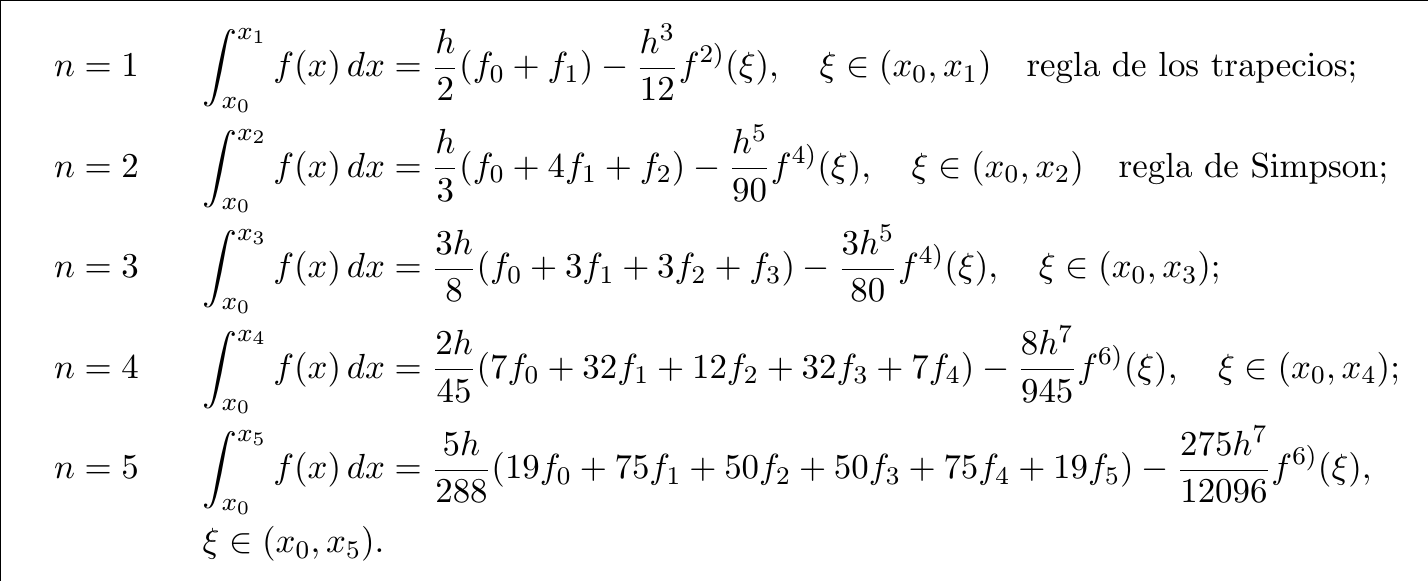
\includegraphics[width=0.95\linewidth]{tema3/formulas-nc-cerradas}
  \end{center}
\end{example}

\begin{example}[Fórmulas de cuadratura abiertas]
  \label{ex:fc-NC-abiertas}
  Sean $x_0,x_1,\cdots,x_n$ los $n+1$ puntos interiores al intervalo
  $[a,b]$ en una f.c. de N--C abierta. Denotemos ahora $x_{-1}=a$,
  $x_{n+1}=b$ y $f_k=f(x_k)$, $k=0,\dots,n$. Procediendo como antes
  se tienen las siguientes fórmulas junto con las expresiones de error
  asociadas:
  \begin{center}
    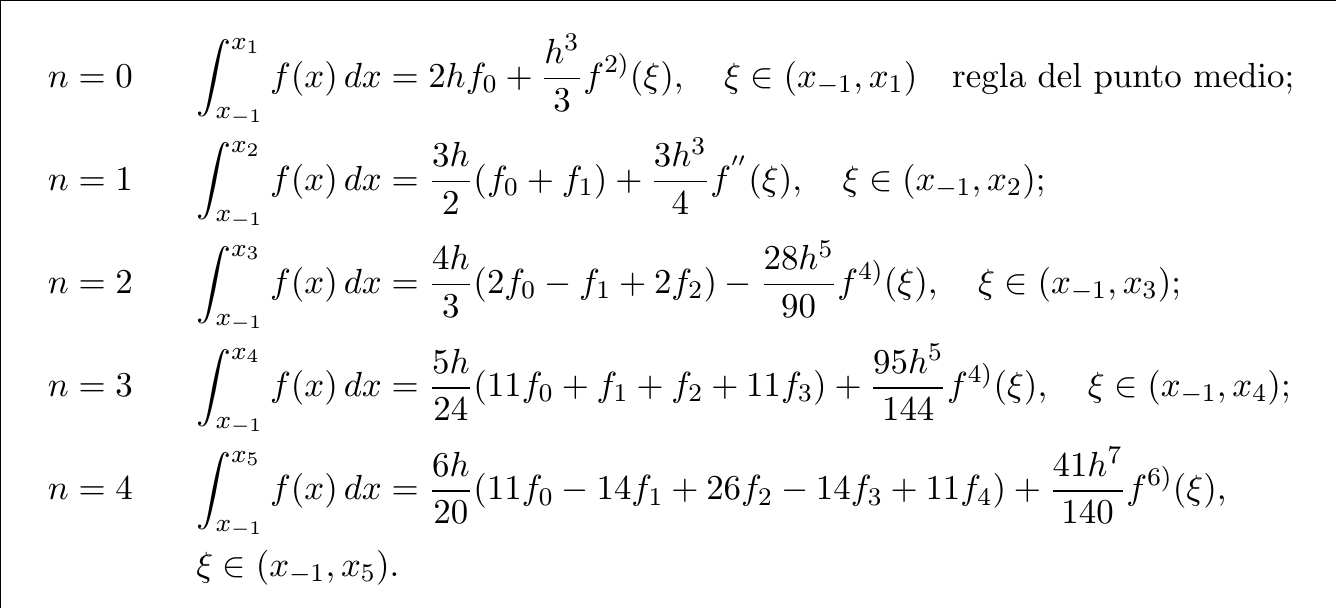
\includegraphics[width=0.95\linewidth]{tema3/formulas-nc-abiertas}
  \end{center}
  Se recomienda, como ejercicio, comprobar estas fórmulas para algunos
  valores de $n$.
\end{example}

\section{Fórmulas de cuadratura compuestas}
\label{sec:fc-compuestas}

A medida que aumenta el número de nodos en las f.c. de N-C, el número
de operaciones necesarias para el cálculo de los pesos comienza a ser
demasiado costoso. Y, lo que es más importante, no podemos asegurar
que, cuando $n\to\infty$, la aproximación $I_n(f)$ converja hacia la
integral de $f$ (de forma similar a lo que ocurre al
aumentar el grado en el polinomio de interpolación de Lagrange). Por
esta razón, en la práctica se usan fórmulas de cuadratura
compuestas (o integración a trozos).

Las fórmulas compuestas se definen de la siguiente forma: sea una
partición del intervalo $[a,b]$, $a=\ox_0<\ox_1<...<\ox_N=b$, que por
simplicidad supondremos uniforme (con $N+1$ puntos
equiespaciados).  Descomponemos
la integral global de $f$ como suma de integrales en cada subintervalo
$[\ox_{i-1},\ox_i]$:
\begin{equation*}
  \int_a^b f(x)\,dx = \sum_{i=1}^N \int_{\ox_{i-1}}^{\ox_i}f(x)\,dx.
\end{equation*}
A continuación aplicamos, en cada uno de estos subintervalos, una
fórmula de cuadratura sobre $n+1$ puntos, con $n\in\Nset$ fijo (en la
práctica se suelen usar fórmulas sencillas, en concreto fórmulas de
N--C con $n=0$, $1$ o $2$). Así, podemos aproximar la integral de $f$
haciendo que $H\to 0$, donde $H=(b-a)/N$ es la longitud de
los subintervalos.

Con más detalle: en el subintervalo $[\ox_{i-1},\ox_i]$ elegimos $n+1$
puntos equiespaciados, $\ox_0^{(i)}<\ox_1^{(i)}<\cdots<\ox_n^{(i)}$, y
consideramos una f.c:
\begin{align}
  \label{eq:fc.compuesta.en.un.intervalo}
  I_n^i(f)&=\sum_{j=0}^n \omega_j^{(i)}f(x_j^{(i)}),
\intertext{en la que el error viene dado (por definición) como:}
  E_n^i(f)&=\int_{\ox_{i-1}}^{\ox_i} f(x)\,dx -  I_n^i(f).
  \label{eq:fc.compuesta.error.subintervalos}
\end{align}
\begin{definition}
  Una fórmula de cuadratura compuesta se define como la suma de las
  f.c. en cada uno de los subintervalos de integración:
  \begin{equation*}
    I_N(f)=\sum_{i=1}^N I_n^i(f)  =\sum_{i=1}^N \sum_{j=0}^n \omega_j^{(i)}f(x_j^{(i)}).
  \end{equation*}
  \label{def:fc.compuesta}
\end{definition}
\subsection*{Expresión del error en fórmulas compuestas}
Si definimos el error de cuadratura en una fórmula compuesta como la
diferencia entre la integral $\int_a^b f(x)\,dx$ y su aproximación
$I_N(f)$, es fácil ver que este error coincide con la suma de los
errores en los $N$ subintervalos $[\ox_{i-1},\ox_i]$:
\begin{alignat*}{2}
  E_N(f)&= \int_a^b f(x)\,dx - I_N(f)
  &\quad \text{(definición del error de integración)}
  \\
  &= \sum_{i=1}^N \int_{\ox_{i-1}}^{\ox_i} f(x)\,dx -
  \sum_{i=1}^NI_n^i(f)
  &\text{(definición de una f.c. compuesta)}
  \\
  &= \sum_{i=1}^N\left(
    \int_{\ox_{i-1}}^{\ox_i} f(x)\,dx -  I_n^i(f) \right)
  =\sum_{i=1}^N E_n^i(f)
  &\text{(def. error en subintervalos~(\ref{eq:fc.compuesta.error.subintervalos}))}.
\end{alignat*}

Si acotamos los errores $E_n^i(f)$ que aparecen en el sumatorio
anterior utilizando la cota genérica del error de
cuadratura~(\ref{eq:cota-error-fcti}), podemos obtener una primera
estimación del error de cuadratura $E_N(f)$ (esta tarea se deja como
ejercicio).

Pero en el caso habitual estaremos utilizando fórmulas de N--C en cada
subintervalo, es decir con nodos equiespaciados, y por tanto nos
encontraremos con una situación más favorable: podemos identificar los
errores $E_n^i(f)$ usando el teorema~\ref{thm:error.formulas-nc}, en
concreto la expresión~(\ref{eq:error-formulas-nc}), llegando al
siguiente resultado:

\begin{theorem}
  \label{thm:cota.error.fc.compuestas-nc}
  Sea $I_N$ una f.c. compuesta sobre una partición uniforme
  $a=\ox_0<\ox_1<...<\ox_N=b$. Supongamos que $I_N$ está definida por una
  fórmula de N--C de $n+1$ puntos en cada subintervalo
  $[\ox_{i-1},\ox_i]$.  Si $f\in C^k([a,b])$, donde $k=n+2$ si $n$ es par
  y $k=n+1$ si $n$ es impar, entonces existe $\xi\in(a,b)$ tal que:
  \begin{equation}
    \label{eq:error.fc.compuesta-NC}
   E_N(f)= \int_a^bf(x)\,dx - I_N(f)
   = C_n \, (b-a) \, H^{k} \, f^{k)}(\xi),
  \end{equation}
  donde $H=(b-a)/N$ y $C_n$ es una constante universal (independiente
  de $f$ y del intervalo $[a,b]$). En concreto:
  \begin{equation*}
  C_n=\left\{
    \begin{array}{cl}
      \displaystyle\frac{\gamma_n}{n^k\,k!} & \quad \text{ si la fórmula de N--C es
        cerrada},
      \\ \noalign{\medskip}
      \displaystyle\displaystyle\frac{\gamma_n}{(n+2)^k\,k!} &\quad \text{ si la fórmula
        de N-C es abierta},
    \end{array}
  \right.
\end{equation*}
  donde $\gamma_n$ son las constantes definidas en el
  teorema~\ref{thm:error.formulas-nc}.
\end{theorem}

\begin{proof}~
  Hemos visto que $E_n(f)=\sum_{i=1}^N E_n^i(f)$.
  Si utilizamos la expresión~(\ref{eq:error-formulas-nc}) para el
  error $E_n^i(f)$ en el intervalo $[\ox_{i-1},\ox_i]$ llegamos
  literalmente a:
  \begin{equation}
    E_N(f)=\sum_{i=1}^N E_n^i(f) =\sum_{i=1}^N \gamma_n
    h^{k+1} \frac{f^{k)}(\xi_i)}{k!}  = \gamma_n \frac{
      h^{k+1}}{k!} \sum_{i=1}^Nf^{k)}(\xi_i),
    \label{eq:fc.1}
  \end{equation}
  donde $\gamma_n$, $h$ y $k$ vienen dados en el
  teorema~\ref{thm:error.formulas-nc} y $\xi_i\in(\ox_{i-1},\ox_i)$.

  Veamos que
  \begin{equation}
    \label{eq:fc.7}
    \text{$\exists \xi\in(a,b)$ tal que }
    \frac 1N \sum_{i=1}^Nf^{k)}(\xi_i) = f^{k)}(\xi).
  \end{equation}
  Como $f\in C^k([a,b])$, $f^{k)}$ es continua en $[a,b]$ y por lo
  tanto alcanza todos los valores entre su mínimo y su máximo. Sean
  $m_k=\min_{x\in[a,b]} f^{k)}(x)$ y $M_k=\max_{x\in[a,b]}
  f^{k)}(x)$. Entonces, como para todo $\xi_i$ se tiene que $m_k\le
  f^{k)}(\xi_i)\le M_k$, deducimos que
  $$
  m_k \le \frac 1N \sum_{i=1}^Nf^{k)}(\xi_i) \le M_k,
  $$
  luego se verifica~(\ref{eq:fc.7}). Finalmente, aplicando~(\ref{eq:fc.7}) a~(\ref{eq:fc.1}) y usando que, por definición de $H$, $N=(b-a)/H$:
  \begin{equation}
    \label{eq:fc.8}
    E_N(f) = \gamma_n \frac{
      h^{k+1}}{k!} N f^{k)}(\xi) =   \gamma_n \frac{
      h^{k+1}}{k!}\; \frac{b-a}{H} \,  f^{k)}(\xi).
  \end{equation}

  Para terminar, en función
  del tipo de fórmula de N-C usada en los subintervalos
  $[\ox_{i-1},\ox_i]$, es fácil relacionar $h$ con $H$. En concreto:
  \begin{align*}
    \intertext{\quad $\bullet$ Si la f.c. N--C es \emph{cerrada}:
      $h=(\ox_i-\ox_{i-1})/n=H/n$. Sustituyendo en~(\ref{eq:fc.8}):}
    E_N(f) &= \gamma_n \, (b-a)\, \frac{H^{k}}{n^k\,k!} \,
    f^{k)}(\xi).
    \intertext{\quad $\bullet$ Si la
      f.c. N--C es \emph{abierta}: $
      h=(\ox_i-\ox_{i-1})/(n+2)=H/(n+2)$ luego}
    E_N(f) &= \gamma_n
    \, (b-a) \, \frac{H^{k}}{(n+2)^k\,k!} \, f^{k)}(\xi).
  \end{align*}
  En cualquiera de los dos casos, si definimos $C_n$ como se
  indica en el enunciado del teorema, llegamos a~(\ref{eq:error.fc.compuesta-NC}).
\end{proof}

Algunas observaciones sobre el teorema anterior:
\begin{enumerate}
\item La expresión del error~(\ref{eq:error.fc.compuesta-NC}) nos
  indica que
  \begin{equation*}
    |E_n(f)| \le C_n (b-a) H^k \|f^{k)}\|_{\infty,a,b},
  \end{equation*}
  lo que
  garantiza la convergencia de $I_N(f)$ hacia $\int_a^b f(x)\, dx$
  cuando $H\to 0$ (o, equivalentemente, cuando $N=(b-a)/H \to\infty$).
\item Más aún, la cota anterior nos indica cuál es exactamente la
  velocidad de convergencia en una f.c. compuesta (definida por una
  fórmula de N-C):
  \begin{equation*}
      E_N(f)=O(H^{k}), \quad \text{cuando } H\to 0,
  \end{equation*}
  donde, donde $O(H^m)$ se define en~(\ref{eq:def.O(h^m)}) y, si la
  fórmula de N-C es elegida inteligentemente ($n$ par), $k=n+2$.
  Obsérvese que el error en una fórmula compuesta se rebaja un orden
  respecto a~(\ref{eq:error-formulas-nc}) (asimilando $H =
  h$, salvo constante), por acumulación de los errores locales
  (cometidos en los subintervalos).
\end{enumerate}

\begin{example}[Fórmula compuesta del punto medio]
  Consideramos la fórmula compuesta definida, en cada subintervalo,
  por la fórmula del punto medio (fórmula de N.C. abierta con $n=0$):
  \begin{equation*}
    \int_{\ox_{i}}^{\ox_{i+1}} f(x)\, dx \approx I_0(f)=
    (\ox_{i+1}-\ox_{i}) \, f\big(\frac{\ox_{i+1}+\ox_{i}} 2 \big), \quad i=0,...,N-1.
  \end{equation*}
  Intentaremos obtener una representación explícita de esta f.c.
  compuesta. Para ello, calculamos $h$ en función de $N$ (usando que
  $\ox_{i+1}-\ox_{i} = (b-a)/N$):
  $$
  h= \frac{\ox_{i+1}-\ox_{i}}2 = \frac{b-a}{2N}.
  $$
  Seguidamente, definimos la partición $\{x_k\}_{k=0}^{2N}$ como
  \begin{equation*}
    \left\{
      \begin{aligned}
        x_{2i} &= \ox_i, \quad i=0,...,N \quad \text{(extremos de los
          intervalos)},
        \\
        x_{2i+1} &= x_{2i}+h \quad i=0,...,N-1
        \quad\text{(puntos medios)}.
      \end{aligned}
      \right.
    \end{equation*}
    Teniendo en cuenta que los puntos medios, $x_{2i+1}$, son los
    nodos de integración y denotando $f_{2i+1}=f(x_{2i+1})$,
    para cada $i=0,...,N-1$ tenemos:
  \begin{equation*}
    \int_{2x_i}^{2x_{i+2}} f(x)\, dx =
    2hf_{2i+1} +
    \frac{h^3}{3}f^{''}(\xi_i), \quad \text{con }
    \xi_i\in(2x_i,2x_{i+2}),
  \end{equation*}
  donde se ha incluido la expresión del error para la fórmula del
  punto medio (como en el ejemplo~\ref{ex:fc-NC-abiertas}). En
  consecuencia:
  \begin{equation*}
    \int_a^b f(x)\,dx = \sum_{i=0}^{N-1} \int_{x_{2i}}^{x_{2i+2}} f(x)\,dx
    = 2h \sum_{i=0}^{N-1} f_{2i+1} + \frac{h^3}{3} \sum_{i=0}^{N-1}f''(\xi_i).
  \end{equation*}
  Para terminar, agruparemos los términos de error en un único
  sumando. Para ello, procedemos como en la demostración de
  ~(\ref{eq:fc.7}), en el teorema anterior (siendo ahora $k=2$) y así
  deducimos que existe $\xi\in(a,b)$ tal que
  $$
  \sum_{i=0}^{N-1}f''(\xi_i)=Nf''(\xi)=\frac{b-a}{2h}f(\xi).
  $$
  Así obtenemos la expresión definitiva para la \textbf{fórmula compuesta del
  punto medio}:
  \begin{equation*}
    \int_a^b f(x)\,dx
    = 2h \sum_{i=0}^{N-1} f_{2i+1} + \frac{(b-a)h^2}{6} f''(\xi).
  \end{equation*}
\end{example}

\begin{example} [Fórmula compuesta de Simpson]
  Consideramos ahora la fórmula compuesta definida, en cada
  subintervalo, $[\ox_{i},\ox_{i+1}]$, con $i=0,...,N-1$, como
   \begin{equation*}
    \int_{\ox_{i}}^{\ox_{i+1}} f(x)\, dx \approx I_1(f)=
    \frac{\ox_{i+1}-\ox_{i}}{6} \, \left[f(\ox_i) +
      4f\left(\frac{\ox_{i}+\ox_{i+1}}{2}\right)+f(\ox_{i+1})\right].
  \end{equation*}
  Como ejercicio se puede comprobar que (procediendo como en el
  ejemplo anterior) se obtiene la siguiente expresión para la fórmula
  compuesta de Simpson:
  \begin{equation*}
    \int_a^b f(x)\,dx
    = \frac{h}{3} \left[
      f_0
      + 2\sum_{i=1}^{N-1} f_{2i}
      + 4\sum_{i=0}^{N-1} f_{2i+1}
      + f_{2N} \right]
    + \frac{(b-a)h^4}{180} f^{4)}(\xi).
  \end{equation*}
\end{example}

\section{Fórmulas de cuadratura de Gauss}
\label{sec:fc-Gauss}
Dada una fórmula de cuadratura $I_n(f)=\sum_{i=0}^n \omega_i f(x_i)$,
para $n+1$ nodos $\{x_i\}\in [a,b]$ que han sido \textit{previamente
  fijados}, en la sección~\ref{sec:cuadratura-interpolatorio} (en
concreto, en la Proposición~\ref{pro:existencia.fcti}) hemos visto que
podemos elegir $n+1$ pesos $\omega_i$ de forma adecuada (de hecho,
$\omega_i=\int_a^b L_i(x)\, dx$, o sea la f.c. debe ser de tipo
interpolatorio) para que la fórmula de cuadratura asociada tenga orden
máximo, en concreto orden $\ge n$.

En la secciones~\ref{sec:formulas-de-newton}
y~\ref{sec:fc-compuestas}, dedicadas respectivamente a las f.c. de
Newton-Côtes y a las f.c. compuestas, nos hemos limitado a escoger
nodos equiespaciados (la elección más sencilla) pero sin que exista
ningún tipo de garantía de que ésta sea la elección óptima. En esta
sección nos preguntaremos si es posible \textit{elegir los nodos de manera
adecuada} para que el orden de la f.c. sea el mayor posible. En
concreto, planteamos el siguiente problema:
\begin{equation}
\label{eq:pb.fc.Gauss}
\tag{P}
\left.
  \begin{aligned}
    &\text{Elegir el soporte $S=\{x_0<x_1<...<x_n\}\subset [a,b]$}
    \\
    &\text{tal que la f.c.t.i. asociada sea de orden máximo.}
  \end{aligned}
\right\}
\end{equation}

\begin{definition}
  Las fórmulas de cuadratura con pesos obtenidos como solución del
  problema~(\ref{eq:pb.fc.Gauss}) reciben el nombre de fórmulas de
  cuadratura de Gauss.
\end{definition}
\subsection*{Aproximación heurística}
Para resolver el problema anterior, intentemos razonar como en la
demostración de la proposición~\ref{pro:existencia.fcti} (en la que se
determinaron de forma óptima los coeficientes $\omega_i=\int_a^b
L_i(x)\, dx$ como solución de un sistema lineal de ecuaciones con
matriz de Vandermonde).


Una f.c. $I_n(f)=\sum_{i=0}^n \omega_i f(x_i)$ tiene orden $m\in\Nset$
si y solo si se verifican $m+1$ ecuaciones:
\begin{alignat*}{2}
  E_n(x^0)&=\int_a^b x^0\, dx -I_n(x^0)&\; =0 \\
  E_n(x^1)&=\int_a^b x^1\, dx -I_n(x^1)&\; =0 \\
  % E_n(x^2)&=\int_a^b x^2\, dx -I_n(x^2)&\; =0 \\
  &~\quad\vdots \\
  E_n(x^m)&=\int_a^b x^m\, dx -I_n(x^m)&\; =0
\end{alignat*}
En esta ocasión, en la f.c. podemos escoger libremente los $n+1$ nodos
$\{x_i\}_{i=0}^n$ y los $n+1$ pesos, $\{\omega_i\}_{i=0}^n$. En total
tenemos a nuestra disposición $2n+2$ incógnitas, por tanto, para que
el sistema de ecuaciones anterior tenga matriz cuadrada, deberá estar
formado por $2n+2$ ecuaciones, es decir, debe ser $m=2n+1$.

Esto significa que podemos aspirar a que las fórmulas de cuadratura de
Gauss tengan orden $2n+1$. El inconveniente es que en este caso, el
sistema de ecuaciones no es lineal por lo que, salvo en casos
sencillos, no será posible recurrir esta estrategia simple
para calcular los nodos de integración.


\begin{example}
  Dado el intervalo $[a,b]=[-1,1]$, buscamos dos puntos $x_0,x_1\in
  [a,b]$ y dos pesos $\omega_i\in\Rset$ tales que la f.c. asociada sea
  de orden máximo, $2n+1=3$. Para ello, imponemos que esta f.c. sea exacta
  para los polinomios $x^i$, $i=0,...,3$:
  \begin{alignat*}{3}
    E_n(x^0)&=\int_{-1}^1 x^0\, dx - I_n(x^0)\ =\ 0 \ \Leftrightarrow
    \quad & 2 &= \omega_0+\omega_1,\\
    E_n(x^1)&=\int_{-1}^1 x^1\, dx - I_n(x^1)\ =\ 0 \ \Leftrightarrow
    \quad & 0 &=  \omega_0x_0+\omega_1x_1,\\
    E_n(x^2)&=\int_{-1}^1 x^2\, dx - I_n(x^2)\ =\ 0 \ \Leftrightarrow
    \quad & \frac{2}{3} &= \omega_0x_0^2+\omega_1x_1^2,\\
    E_n(x^3)&=\int_{-1}^1 x^3\, dx - I_n(x^3)\ =\ 0 \ \Leftrightarrow
    \quad &0 &=
    \omega_0x_0^3+\omega_1x_1^3.
  \end{alignat*}
  De la segunda y la cuarta ecuaciones deducimos que o bien
  $\omega_0=\omega_1=1$ o bien $\omega_0=1, \omega_1=-1$.
  Pero teniendo en cuenta la primera ecuación, la única posibilidad es
  $\omega_0=\omega_1=1$. Entonces, según la segunda y la tercera ecuación,
  $x_0=\frac{1}{\sqrt 3}$, $x_1=-\frac{1}{\sqrt 3}$.

  Por lo tanto, la fórmula de cuadratura de Gauss con dos puntos en el
  intervalo $[-1,1]$ (de orden $2n+1=3$) se puede expresar de la
  siguiente forma:
  \begin{equation*}
    \int_{-1}^1 f(x)\, dx \approx f\Big( \frac{-1}{\sqrt 3} \Big)
    + f\Big(\frac{1}{\sqrt 3}\Big).
  \end{equation*}
\end{example}


Para finalizar, y simplemente como orientación (debido a las
características de esta asignatura no podemos entrar en detalles), se
expresa el siguiente resultado sobre existencia y unicidad de fórmulas
de cuadratura de Gauss:
\begin{theorem}~
  \begin{enumerate}
  \item En un intervalo $[a,b]$ existe una única f.c.t.i. de orden $(2n+1)$.
  \item Esta fórmula se corresponde con:
    \begin{enumerate}
    \item El soporte $S=\{x_0<x_1<...<x_n\}$ formado por las $n+1$
      raíces de cierto polinomio (el $(n+1)$--ésimo polinomio
      ortogonal\footnote{Véase [Guillén-Dubova] en bibliografía} en $L^2(a,b)$).
    \item Los pesos, dados por $\omega_i=\int_a^b L_i(x)\, dx$, que son
      todos positivos.
    \end{enumerate}
  \end{enumerate}
\end{theorem}



% \subsection*{Polinomios ortogonales}
% En fórmulas de cuadratura de Gauss, en vez de la resolución de los
% sistemas no lineales descritos anteriormente, calcularán los nodos
% óptimos como raíces de unas familias de polinomios conocidos como
% polinomios ortogonales.

% \begin{definition}
%   \label{def:pol-orgotonales}
%   Consideremos el espacio vectorial $\Pol_n[x]$, formado por los
%   polinomios de grado menor o igual que $n$. Una base
%   $\{\phi_0,\phi_1,\dots,\phi_n\}$ de $\Pol_n[x]$ (donde cada $\phi_i$
%   tiene grado exactamente igual a $n$) se dice ortogonal en
%   $[a,b]$
%   \begin{equation*}
%     \int_a^b \phi_i(x) \phi_j(x)\, dx = 0 \quad \text{si } i\neq j.
%   \end{equation*}
%   Una base se dice ortonormal cuando es ortogonal y además los
%   polinomios son unitarios, en el siguiente sentido:
%   \begin{equation*}
%     \int_a^b (\phi_i(x))^2 \,dx = 1.
%   \end{equation*}
% \end{definition}

% \begin{proposition}
%   Para todo $n\ge 0$ existen bases ortogonales,
%   $\{\phi_0,\phi_1,\dots,\phi_n\}$, de $\Pol_n[x]$, que se pueden
%   construir mediante el siguiente algoritmo, conocido como método de
%   ortogonalización de Gram-Schmidt:
%   \begin{quotation}
%     Dada una base (no necesariamente ortogonal),
%     $\{\varphi_0,\varphi_1,\dots,\varphi_n\}$ de $\Pol_n[x]$,
%     definimos
%     \begin{align*}
%       \phi_0 &= \varphi_0,\\
%       \phi_1 &= \varphi_1 -
%       \frac{\int_a^b\phi_0\varphi_1}{\int_a^b\phi_0^2} \phi_0\\
%       &\ \vdots\\
%       \phi_n &= \varphi_n -
%       \frac{\int_a^b\phi_{n-1}\varphi_n}{\int_a^b\phi_{n-1}^2} \phi_{n-1}\\
%     \end{align*}
%   \end{quotation}
% \end{proposition}

% \begin{proof}
%   Es fácil comprobar que el conjunto $\{\phi_0,\phi_1,\dots,\phi_n\}$
%   construido mediante el método de Gram-Schmidt es ortogonal.
% \end{proof}

% % \begin{proposition}
% %   Dadas dos bases ortogonales de $\Pol_n[k]$,
% %   $\{\phi_0,\phi_1,\dots,\phi_n\}$ y
% %   $\{\overline\phi_0,\overline\phi_1,\dots,\overline\phi_n\}$ los
% %   polinomios de cada una de estas bases son proporcionales, es decir,
% %   para cada $i=0,...n$ existe $\alpha_i$ tal que
% %   \begin{equation*}
% %     \phi_i = \alpha_i ,\overline\phi_i.
% %   \end{equation*}
% %   En particular, $\phi_i$ y $\overline\phi_i$ tienen los mismos
% %   ceros.
% % \end{proposition}

% \begin{theorem}
%   Sea $\{\phi_0,\phi_1,\dots,\phi_n\}$ un conjunto de polinomios
%   ortogonales en $[a,b]$. Entonces cada polinomio $\phi_k$ tiene
%   exactamente $k$ raíces reales simples $\{x_0<x_1<...<x_k\}$ en
%   $(a,b)$.
% \end{theorem}

% \begin{theorem}
%   Existe una única f.c.t.i. de orden $(2n+1)$. Esta fórmula se
%   corresponde con el soporte $S=\{x_0<x_1<...<x_n\}$ formado por las
%   $n+1$ raíces de $\phi_{n+1}$, el $n$--ésimo polinomio ortogonal en
%   $(a,b)$. Además, los pesos $\omega_i=\int_a^b L_i(x)\, dx$ son todos
%   positivos.
% \end{theorem}


\begin{EjerciciosPropuestos}
  \begin{problema}
    Deducir la fórmula compuesta de los trapecios, así como su
    expresión del error. Utilizando esta fórmula, calcular una
    aproximación de la integral
    $$
    \int_0^1 \log(1+x^2)\, dx
    $$
    en la que podamos garantizar que el error de cuadratura es menor que
    $\varepsilon=0.001$. ¿En cuántos subintervalos hay que dividir el
    intervalo $[0,1]$?
  \item Se considera la fórmula de cuadratura
    \begin{equation*}
      \int_0^1 f(x)\,dx \approx c_0 f(0) + c_1 f\bigg(\frac{1}{3}\bigg)
      + c_2 f\bigg(\frac{2}{3}\bigg) + c_3 f(1).
    \end{equation*}
    \begin{itemize}
    \item Calcular los coeficientes $c_0$, $c_1$, $c_2$ y $c_3$ para
      los que la fórmula de cuadratura es exacta para polinomios de
      grado menor o igual que $3$. Comprobar que la fórmula resultante
      no proporcionan el valor exacto para polinomios de orden $4$.
    \item Aplicar esta fórmula de cuadratura para aproximar la
      siguiente integral:
      \begin{equation*}
        \int_0^1 \big(-\log(\cos x) \big)\,dx
      \end{equation*}
    \item Realizar el cambio de variables $t=(x-a)/(b-a)$ para
      transformar la integral
      \begin{equation*}
        \int_a^b f(x)\, dx
      \end{equation*}
      en una integral sobre el intervalo $[0,1]$. Utilizar la fórmula
      de cuadratura del apartado anterior para deducir una
      regla de cuadratura en cualquier intervalo $[a,b]$.
    \item Sabiendo que la regla anterior es la fórmula de cuadratura
      de Newton-Côtes cerrada con $4$ nodos, obtener una expresión que
      de la fórmula compuesta correspondiente, que permita aplicarla.
    \item Aplicar la fórmula compuesta con $20$ subintervalos para
      aproximar la siguiente integral:
      \begin{equation*}
        \int_0^{10} \log\big(1+3e^{-x^2}\big)\,dx.
      \end{equation*}
    \end{itemize}
  \end{problema}

  \begin{problema}
  Determinar las constantes $A_0$, $A_1$ y $A_2$ de modo que la
  fórmula de cuadratura
  \begin{equation*}
    \int_0^h f(x)\,dx = h \bigg\{
    A_0f(0) + A_1f\bigg(\frac{h}{3}\bigg) + A_2 f(h) \bigg\}
  \end{equation*}
  sea exacta para polinomios del mayor grado posible. Utilizarla para
  aproximar la integral
  \begin{equation*}
    \int_0^{1/2} e^{-x^2}\, dx.
  \end{equation*}
  \end{problema}

  \begin{problema}
    Determinar los coeficientes $\alpha_0$, $\alpha_1$,  $\beta_0$ y
    $\beta_1$ para los que la fórmula de cuadratura
    \begin{equation*}
      \int_a^b f(x)\, dx \approx \alpha_0 f(a) + \alpha_1 f(b)
      + \beta_0 f'(a) + \beta_1 f'(b)
    \end{equation*}
    tiene el mayor orden posible. ¿Cuál es este orden de precisión?.
    Sabiendo que el error puede escribirse como
    \begin{equation*}
      \gamma (b-a)^5 f^{4)}(\xi),
    \end{equation*}
    para algún $\xi\in(a,b)$, determinar el valor de $\gamma$.
  \end{problema}

  \begin{problema}
    Para calcular un valor aproximado de $\ln 2$, se utilizará el
    hecho de que la integral
    \begin{equation*}
      \int_1^2 \frac{1}{x}\, dx
    \end{equation*}
    concide con este valor. Averiguar el número de subintervalos
    necesarios para que, al usar la fórmula compuesta de Simpson, el
    error sea inferior a $10^{-3}$. Utilizando el ordenador, calcular
    una aproximación de $\log 2$ y comprobar el error.
  \end{problema}

  \begin{problema}
    Se considera la fórmula de cuadratura
    \begin{equation*}
      \int_0^1 f(x)\, dx \approx A (f(x_0) + f(x_1)).
    \end{equation*}
    \begin{enumerate}
    \item Hallar el valor de $A$, $x_0$ y $x_1$ para que la
      fórmula sea exacta para polinomios del mayor grado
      posible. ¿Cuál es éste?
    \item Comprobar, mediante el cambio de variables $t=2x-1$, que
      la fórmula de cuadratura coincide con la regla de Gauss con
      dos nodos:
      \begin{equation*}
        \int_{-1}^1 g(x)\,dx \approx g\bigg(\frac{-1}{\sqrt
          3}\bigg) + g\bigg(\frac{1}{\sqrt 3}\bigg).
      \end{equation*}
    \end{enumerate}
  \end{problema}

  \begin{problema}
    La regla de Lobatto es una fórmula de cuadratura gaussiana
    definida en $[-1,1]$ de la siguiente forma:
    \begin{equation*}
      \int_{-1}^1 f(x)\, dx = A_0 f(-1) + \sum_{i=1}^{n-1} A_if(x_i) +
      A_nf(1).
    \end{equation*}
    \begin{itemize}
    \item Detallar la expresión de la regla de Lobatto para
      $n=3$. ¿Cuál es el orden de precisión de esta regla?
    \item Realizando un cambio de variable adecuado, utilizar la regla
      de Lobatto (con $n=3$) para estimar
      \begin{equation*}
        \int_1^2 e^x\, dx.
      \end{equation*}
    \end{itemize}
  \end{problema}
\end{EjerciciosPropuestos}

\end{document}

% ===============
=======

\begin{problemas}
  \begin{problema}
    Demostrar que la función $f(x)=x^2e^{x}-1$ tiene un único
    cero. Utilizar el método de bisección para aproximarlo con un
    error menor que $\varepsilon=10^{-7}$. Comparar el resultado con
    la solución aproximada que proporciona la función \texttt{fsolve}
    (contenida en el paquete \texttt{optimize} de \textit{Scipy}).
  \end{problema}
  \begin{problema}
    Utilizar el método de bisección para aproximar las raíces de las
    siguientes ecuaciones con una tolerancia menor que
    $\varepsilon=10^{-8}$.
    \begin{enumerate}
    \item $e^x-3x^2=0$.
    \item $x^3=x^2+x+1$.
    \end{enumerate}
  \end{problema}
 \begin{problema}
    Consideremos el siguiente producto infinito para el cálculo de $\pi$:
    (publicado en 1593 por François Viète y conocido como fórmula de Viète):
    \begin{equation*}
      \frac{2}{\pi}  = \prod_{k\to\infty} \frac{a_k}2, \qquad\text{donde }\quad
      a_0 = \sqrt{2}, \quad a_{k+1} = \sqrt{2+a_k}.
    \end{equation*}

    \begin{enumerate}
    \item Calcular las $15$ primeras aproximaciones de $\pi$ para la
      fórmula de Viète (correspondientes a la evaluación del producto
      anterior para $k=0,...,14$) y sus errores absolutos, $e_k$.
    \item Mostrar en una tabla los logaritmos de los errores, $\log
      e_k$, y los cocientes $\log e_{k+1}/\log
      e_{k}$ (con $k\ge 0$).
    \item Justificar la siguiente afirmación y utilizarla para estimar
      el orden de la fórmula de Viète:
      \begin{equation*}
        \label{eq:1}
        \{x_k\} \text{ es un método iterativo de orden } p
        \Leftrightarrow \lim_{k\to\infty} \frac{\log e_{k+1}}{\log e_{k}}=p.
      \end{equation*}
    \end{enumerate}
  \end{problema}
  \begin{problema}
    Consideremos el problema de punto fijo $x=g(x)$, con
    $g(x)=1/(2+x)$.  Probar que existe una única solución en el
    intervalo $[0,1]$ y que método de aproximaciones sucesivas
    $x_{k+1}=g(x_k)$ converge hacia una solución para cualquier
    inicialización, $x_0\in[0,1]$. Aproximar la
    solución con un error menor que $\varepsilon=10^{-8}$.
  \end{problema}
  \begin{problema}
    Dada la ecuación $f(x)=e^x-(x+1)^2=0$:
    \begin{itemize}
    \item Estudiar sus raíces reales
    \item Localizarlas en intervalos en los que el método de Newton
      esté bien definido y sea convergente (idea: en cada intervalo,
      aplicar la regla de Fourier)
    \item En cada uno de estos intervalos, calcular una aproximación
      de la raíz de forma que el error con la solución exacta sea
      menor que $10^{-6}$.
    \end{itemize}
  \end{problema}
  \begin{problema}
    Calcular mediante el método de Newton las raices de
    $$f(x)=2\sqrt{x}-\frac{x^3+5}{5}$$ en $[0.1,1]$ realizando
    iteraciones hasta que la diferencia en dos etapas consecutivas sea
    menor que $10^{-10}$. ¿Converge el método si partes del punto
    medio del intervalo? Justifícalo geométricamente. ¿Y desde los
    extremos? Justifícalo mediante la Regla de Fourier.
  \end{problema}
  \begin{problema}
    Dada la ecuación $f(x)=e^x-(x-2)^2=0$:
    \begin{itemize}
    \item Justificar geométricamente que sólo posee una raíz real
    \item Demostrarlo analíticamente. Idea: probar que $f'(x)>0$ para
      todo $x\in\Rset$. Para ello, cuando $x>2$, aplicar a $e^x$ el
      teorema del valor medio en $[2,x]$ para probar que $e^x>2(x-2)$.
    \end{itemize}
  \end{problema}
  \begin{problema}
    Calcular las tres primeras aproximaciones ($k=0,1,2$) de $\pi$
    mediante el algoritmo de Gauss-Legendre (o de Brent-Salamin):
    $a_0=1$, $b_0=1/\sqrt 2$, $t_0=1/4$, $p_0=1$,
    \begin{align*}
      a_{k+1}&=(a_{k}+b_{k})/2 , &\quad
      t_{k+1}&=t_k - p_k(a_k -a_{k+1})^2, \\
      b_{k+1}& =\sqrt{a_{k}\*b_{k}}, &\quad p_{k+1}&=2p_k.
    \end{align*}
    $$
    \pi = \lim_{k\to\infty} \frac{(a_k+b_k)^2}{4t_k}.
    $$
    Utilizando los logaritmos de los errores absolutos, estimar el
    orden del algoritmo.
  \end{problema}
  \begin{problema}
    Consideremos el método de bisección para
    una función $f$ en el intervalo $[a,b]=[2.6,4.2]$.
    \begin{enumerate}
    \item ¿Cuál es la longitud del subintervalo en el paso $k$--ésimo?
    \item ¿Cuál es la máxima distancia entre la raíz, $\alpha$, de $f$
      y el punto medio del intervalo en ese paso $k$--ésimo?
    \item ¿Cuántas iteraciones son necesarias, como mínimo, para que
      la longitud del intervalo sea menor que $\varepsilon=10^{-5}$?
    \end{enumerate}
  \end{problema}
\end{problemas}
%%% Local Variables:
%%% mode: latex
%%% TeX-master: "../apuntes-MNII.tex"
%%% End:


% \stepcounter{chapter}
% *#06#
%
% imei
% 359 778 047 841 331
%
\renewcommand{\tt}{t}
\newcommand{\yy}{y}
\newcommand{\yn}{{\yy_n}}
\newcommand{\ynn}{{\yy_{n+1}}}
\newcommand{\ta}{a}
\newcommand{\tb}{b}
\newcommand{\tn}{{\tt_n}}
\newcommand{\tnn}{{\tt_{n+1}}}
\newcommand{\zn}{{z_n}}
\newcommand{\znn}{{z_{n+1}}}
\newcommand{\ycero}{{y_a}}
% \newcommand{\sol}{\varphi}
\newcommand{\sol}{g}
\newcommand{\lipschitz}{$y$--Lipschitz\xspace}
\newcommand{\locLipschitz}{localmente \lipschitz}
\newcommand{\globLipschitz}{\lipschitz}
\newcommand{\errCons}{{\cal E}}
\newcommand{\RK}{Runge--Kutta\xspace}
\newcommand{\AB}{Adams--Bashforth\xspace}
\newcommand{\AM}{Adams--Moulton\xspace}


\section{Introducción}

Son muy numerosos los problemas (con orígenes diversos como la física,
química, biología o economía) que se formulan matemáticamente en
términos de ecuaciones diferenciales, es decir, ecuaciones cuya
incógnita, una función $y(x)$, describe un fenómeno dado a través de
una ley que relaciona a esta función con sus derivadas. La formulación
adecuada de esta ley junto a algunos datos adicionales (condiciones
iniciales) garantizarán el buen planteamiento del problema.

Este tema se centra en la resolución numérica de problemas de valor
inicial (o problemas de Cauchy) asociados a ecuaciones diferenciales
ordinarias (EDO). Este tipo de problemas se escriben de la siguiente
forma:
\begin{equation}
  \label{eq:pvi}
  \tag{PVI}
  \left\{
  \begin{aligned}
    &y' = f(\tt,\yy), \quad \tt\in[\ta,\tb],
    \\
    &y(\ta) = \ycero,
  \end{aligned}
  \right.
\end{equation}
donde la función (continua) $f:[\ta,\tb]\times\Rset\to\Rset$ y el
estado inicial $\ycero\in\Rset$ son datos conocidos. En el próximo
tema se estudiará el caso general, donde
$f:[\ta,\tb]\times\Rset^n\to\Rset^n$ e $\ycero\in\Rset^n$, con
$n\in\Nset$. Se ha optado por denotar $t\in [a,b]$ a la variable
independiente.  En numerosos problemas de la ciencia y la ingeniería,
esta variable representa el tiempo y, aunque no siempre es
sea así, en muchas ocasiones puede ser conveniente
hablar de $\tt$ como la <<variable temporal>>).

\begin{definition}
  \label{def:sol-pvi}
  Llamamos solución de~\eqref{eq:pvi} a toda función $\sol\in
  C^1([\ta,\tb])$ tal que $\sol'(\tt)=f(\tt,\sol(\tt))$ para todo
  $\tt\in[\ta,\tb]$ y además $\sol(\ta)=\ycero$.\label{def:3}
\end{definition}

Nota: con frecuencia, denotaremos por $y(t)$ o $y(x)$ a la solución (como
  en numerosos recursos bibliográficos).

Obsérvese que, según esta definición, el concepto de solución tiene un
sentido global (en todo el intervalo $[a,b]$), y no local (en un entorno
de $\ta$). Como paso previo a la resolución numérica
de~\eqref{eq:pvi}, deberemos garantizar que este problema está bien
planteado, es decir asegurar la existencia y unicidad de solución
de~(\ref{eq:pvi}), en el sentido de la definición~\ref{def:sol-pvi}.

\section{Resultados teóricos preliminares}
\label{sec:tema4:resultados-teoricos}

Antes de comenzar a estudiar métodos numéricos para la resolución de
problemas de Cauchy, recordaremos en esta sección algunos
resultados relacionados con la existencia y unicidad de solución
de~(\ref{eq:pvi}), que resultarán útiles para garantizar existencia de
solución en los problemas que aparecerán en las siguientes secciones.
La clave en estos resultados será el analizar si la función $f(x,y)$
verifica la condición de Lipschitz que se define a continuación:

\begin{definition}
  \label{def:lipschitz}
  Decimos que una función $f(\tt,y)$ verifica la condición de
  \resaltar{Lipschitz uniformemente} (o globalmente) respecto a $y$ en
    $[\ta,\tb]$ (o simplemente que $f$ es \globLipschitz)
    si existe $L>0$ tal que
  \begin{equation*}
    |f(\tt,y) - f(\tt,z)| \le L |y-z|, \quad \forall \tt\in [\ta,\tb],
    \quad  \forall y,z\in \Rset.
  \end{equation*}
  Decimos que una función $f(\tt,y)$ verifica la condición de
  \resaltar{Lipschitz localmente} respecto a $y$ en
  $[\ta,\tb]$ (o que $f$ es \locLipschitz) si para todo compacto
  $K\subset\Rset$ existe $L_K>0$ tal que
  \begin{equation*}
    |f(\tt,y) - f(\tt,z)| \le L_K |y-z|, \quad \forall \tt\in [\ta,\tb],
    \quad  \forall y,z\in K.
  \end{equation*}
\end{definition}

Fijaremos la siguiente
\textbf{notación}: $\dy f$ designará a la derivada parcial de $f$
respecto a $y$, es decir $\dy f(\tt,y) = \frac{\partial f}{\partial
  \yy}(\tt,y)$. Para el resto de las variables se usarán notaciones
similares.
  En la práctica, para estudiar si una función es (local o
  globalmente) Lipschitz se suelen usar las siguientes condiciones:
  \begin{proposition}~
    \begin{enumerate}
    \item Si $\dy f$ es continua en $[\ta,\tb]\times\Rset$, entonces
      $f$ es \locLipschitz.
    \item Si $\dy f$ es continua y además está acotada en
      $[\ta,\tb]\times\Rset$, entonces $f$ es uniformemente
      \globLipschitz.
    \item Recíprocamente, si $\dy f$ es continua y $f$ es
      uniformemente \globLipschitz, entonces $\dy f$ está acotada en
      $[\ta,\tb]\times\Rset$.
    \end{enumerate}
  \end{proposition}
  \begin{proof}
    Tan solo comprobaremos la segunda de estas afirmaciones. El resto
    de ellas se deja como ejercicio\footnote{Indicación: primera
      afirmación se demuestra de forma análoga (usando que $\dy f$
      está acotada en todo compacto $K\subset\Rset$) mientras que la
      tercera se basa en la definición de derivada parcial, que se
      puede acotar usando la condición de Lipschtiz.}.

    Supongamos $\dy f$ es
    continua en $[\ta,\tb]\times\Rset$. Entonces en cada <<instante>>
    $t\in[\ta,\tb]$ la función
  $$\dy f(t,\cdot):\Rset \to \Rset$$
  es continua. Aplicando el teorema del valor medio, se tiene que
  dados $y$, $z\in\Rset$ existe $y^*$ entre $y$ y $z$ tal que
  \begin{equation*}
    |f(\tt,y)-f(\tt,z)| = |\dy f(\tt,y^*) \cdot (y-z)|=|\dy f(\tt,y^*)| \cdot |y-z|.
  \end{equation*}
  Como además $\dy f$ está acotada, existe $L>0$ tal que
  $|\dy f(\tt,y)|\le L$ para todo $(\tt,y)\in [\ta,\tb]\times\Rset$ y
  entonces
  \begin{equation*}
    |f(\tt,y) - f(\tt,z)| \le L |y-z|.
  \end{equation*}
\end{proof}

\begin{example}
  La función $$f(x,y)=y^2$$ es \locLipschitz en cualquier intervalo
  $[\ta,\tb]$, pues su derivada parcial $\dy f(x,y)=2y$ es continua. Sin
  embargo, esta función no está acotada cuando $y\in\Rset$, por lo que
  no tenemos garantías de que $f(x,y)$ sea uniformemente \globLipschitz.

  Veamos que realmente $f(x,y)$ no es uniformemente \globLipschitz,
  comprobando que para cualquier constate $L>0$, podemos encontrar dos
  valores, $y_L$, $z_L\in\Rset$ de forma que
  \begin{equation*}
  |f(\tt,y_L)-f(\tt,z_L)| >  L  |y_L-z_L|.
 \end{equation*}
 En concreto, dada $L>0$ tomamos $y_L=2L$ y $z_L=0$. Así
 \begin{align*}
   L|y_L-z_L|&=2L
   \intertext{y evaluando $|f(\tt,y_L) - f(\tt,z_L)|$ tenemos que, para todo $\tt\in[a,b]$:}
   |f(\tt,y_L)-f(\tt,z_L)|&=|(2L)^2-0^2|=4L^2 > 2L^2 =  L|y_L-z_L|.
 \end{align*}
\end{example}


A continuación se resumen los resultados teóricos fundamentales de
existencia y unicidad para problemas de Cauchy. El primero utiliza
hipótesis más débiles (\locLipschitz), aunque sin alcanzar
directamente la existencia y unicidad de solución global en todo
$[a,b]$. El Teorema~\ref{thm:existencia-unif-lipschitz} garantiza la
existencia y unicidad de solución de~\eqref{eq:pvi} en $[a,b]$, aunque
a costa de imponer una hipótesis muy fuerte (Lipschitz uniforme), que
reduce considerablemente el rango de problemas diferenciales
abarcados.
\begin{proposition}
  \label{thm:existencia-loc-lipschitz}
  Sea $f$ continua en $[\ta,\tb]\times\Rset$ y \locLipschitz. Entonces, para
  cualquier inicialización $\ycero\in\Rset$:
  \begin{enumerate}
  \item Existe una única solución local\footnote{Esta propiedad se puede ver como un
      corolario del clásico Teorema de Picard, que garantiza
      existencia y unicidad en un entorno de $a$.} (que definiremos como una
    solución definida sólo en $[\ta,\ta+\varepsilon]$ para algún
    $\varepsilon>0$)
  \item Existe una única solución maximal\footnote{Una solución
      maximal (por la derecha) es una solución local de~(\ref{eq:pvi}), definida en
      $[\ta,\ta+\varepsilon]$, que no es prolongable a ningún
      intervalo $[\ta,c]$ (con $c>\ta+\varepsilon$).}
    de~\eqref{eq:pvi}.
  \item Además: si esta solución maximal $\sol(\tt)$ no está definida en todo
    $[\ta,\tb]$ es porque explota en tiempo finito (es decir existe
    $c\in (\ta,\tb)$ tal que $\lim_{\tt\to c^-} \sol(\tt) = \infty$).
  \end{enumerate}
\end{proposition}

\begin{proposition}
  \label{thm:existencia-unif-lipschitz}
  Sea $f$ continua en $[\ta,\tb]\times\Rset$ y (globalmente) \globLipschitz.
  Entonces, para cualquier inicialización $\ycero\in\Rset$, existe una
  única solución maximal de~\eqref{eq:pvi} (definida en todo el
  intervalo $[\ta,\tb]$).% Además, para todo $\tt\in[\ta,\tb]$
  % se tiene la siguiente desigualdad:
  % \begin{equation*}
  %   |y(\tt)-y(\ta)| \le (\tb-\ta) \Big( \max_{\tt\in[\ta,\tb]}
  %     f(\tt,y(\ta))\Big) e^{L(\tt-\ta)}.
  % \end{equation*}
\end{proposition}


En lo que sigue, estudiaremos el análisis numérico de problemas
diferenciales en los que, en principio, la función $f(\tt,y)$ es tan
solo \locLipschitz. Por tanto el estudio de la existencia de solución
en $[\ta,\tb]$ no será una tarea inmediata. % La técnica usual será
% demostrar que la solución maximal del problema~(\ref{eq:pvi}) está
% acotada en $[\ta,\tb]$ y por tanto no explota en tiempo finito. Así,
% el Teorema~\ref{thm:existencia-loc-lipschitz} garantizará que la
% solución maximal está definida en todo $[\ta,\tb]$ (ver en el
% ejemplo~\ref{ex:existencia-unicidad-loc-lipschitz}).

% Pero demostrar que la solución maximal del problema~(\ref{eq:pvi})
% está acotada en $[\ta,\tb]$ no es fácil. Por tanto, introducimos aquí
% algunas propiedades interesantes de las ecuaciones diferenciales que
% nos pueden resultarán de utilidad para este propósito. Para su
% demostración, consultar la bibliografía.

% \begin{proposition}[Comparación de soluciones de~(\ref{eq:pvi})]
% \label{pro:propiedades-pvi}
%   Bajo las hipótesis del teorema~\ref{thm:existencia-loc-lipschitz}
%   ($f$ \locLipschitz):
%   \begin{enumerate}
%   \item Sean $\sol_1(\tt)$, $\sol_2(\tt)$ las respectivas soluciones
%     de dos problemas del tipo~\eqref{eq:pvi} para la \textbf{misma
%       ecuación diferencial} $y'=f(\tt,y)$ pero con \textbf{distintas
%       condiciones iniciales}, es decir:
%     $$\sol_1(\ta)<\sol_2(\ta)$$
%     Entonces las gráficas de $\sol_1$ e $\sol_2$ no se cortan en
%     ningún punto. En concreto, si $\sol_1$ y $\sol_2$ están
%     definidas, respectivamente, en los intervalos $I_1$ e $I_2$,
%     entonces
%     \begin{equation*}
%       \sol_1(\tt) < \sol_2(\tt), \quad \forall \tt \in I_1
%       \cap I_2.
%     \end{equation*}

%   \item Sean $\sol_1(\tt)$, $\sol_2(\tt)$ las soluciones de dos
%     problemas del tipo~\eqref{eq:pvi} con la \textbf{misma condición
%       inicial} pero con \textbf{ecuaciones diferenciales distintas},
%     $y'=f_1(\tt,y)$, $y'=f_2(\tt,y)$. Si
%     $$
%     f_1(\tt,y) \le f_2(\tt,y) \quad \forall \tt\in[\ta,\tb], \quad
%     \forall y\in\Rset,
%     $$
%     entonces
%     $$
%     \sol_1(\tt)\le \sol_2(\tt) \quad \forall \tt \in
%     I_1 \cap I_2.
%     $$
%   \end{enumerate}
% \end{proposition}

% \begin{example}
%   \renewcommand{\tt}{x}
%   \label{ex:existencia-unicidad-loc-lipschitz}
%   Estudiaremos la existencia y unicidad de solución del siguiente
%   problema de valor inicial:
%   \begin{equation*}
%     \left\{
%       \begin{aligned}
%         &y' = -y^2+2y\,\cos \tt, \quad \tt\in [0,2],\\
%         &y(0)=1.
%       \end{aligned}
%     \right.
%   \end{equation*}
%   En primer lugar, $f(x,y)=-y^2+2y\,\cos \tt$ y
%   $\dy f(t,y)=-2y+2\cos t$ son continuas en $[0,2]\times\Rset$, luego
%   $f$ es \locLipschitz, por lo que (según el
%   teorema~\ref{thm:existencia-loc-lipschitz}) existe una única
%   solución maximal, a la que denominaremos $\sol(\tt)$ definida bien
%   en todo $I=[0,2]$ o bien en $I=[0,c)$ con $c<2$. Pero esta última
%   posibilidad no se verifica, pues entonces $\sol(\tt)$ debería
%   en $c$. Y esto no ocurre porque $\sol(\tt)$ está acotada:
%   \begin{enumerate}
%   \item Sea $\sol_1$ la solución del problema de valor inicial para la
%     misma ecuación diferencial pero para la condición inicial
%     $y(0)=0$. Está claro que su única solución es $\sol_1(\tt)=0$
%     para todo $\tt\in\Rset$. Y como $0=\sol_1(0)<\sol(0)=1$, entonces
%     (según la proposición~\ref{pro:propiedades-pvi}, parte 2) podemos
%     asegurar que $\sol$ está acotada inferiormente:
%     \begin{equation*}
%       0=\sol_1(\tt)<\sol(\tt), \quad \forall \tt\in I.
%     \end{equation*}
%   \item Sea ahora $f_2(\tt,y)=-y^2+2y$. Como $\cos\tt \le 1$  (y como
%     ya podemos suponer $y>0$):
%     $$f(\tt,y)=-y^2+2y\cos\tt \le -y^2+2y = f_2(\tt,y)\quad
%     \forall \tt\in I, \forall y\in\Rset^+.$$
%     Ahora podemos calcular
%     directamente la solución $\sol_2$ del problema de valor inicial
%     $y'=f_2(\tt,y)$, $y(0)=1$ (ya que la ecuación es autónoma),
%     obteniendo:
%     $$
%     \sol_2(\tt)=\frac{2e^{2\tt}}{1+e^{2\tt}},
%     $$
%     función continua y, en consecuencia, acotada superiormente en $[0,2]$.
%     Según la proposición~\ref{pro:propiedades-pvi} (parte 1)
%     \begin{equation*}
%       \sol(\tt)\le\sol_2(\tt),
%     \end{equation*}
%     luego $\sol(\tt)$ está también acotada superiormente en
%     $[0,2]$. Por lo tanto, $\sol$ está definida en todo $[0,2]$.
%   \end{enumerate}
%   \renewcommand{\tt}{t}
% \end{example}


\section{El método de Euler}

A partir de ahora, nuestro objetivo será la descripción, análisis e
implementación de distintos métodos numéricos para la aproximación de
la solución de~\eqref{eq:pvi}. Estos métodos partirán con la
definición de una partición del intervalo $[\ta,\tb]$, formada por
$N+1$ puntos:
\begin{equation*}
  \ta=\tt_0 < \tt_1 < \cdots < \tt_N=\tb.
\end{equation*}
Por simplicidad, supondremos que la partición es uniforme, es decir,
\begin{equation*}
  \text{ si } h=\frac{b-a}{N}, \quad \text{entonces} \quad
  \tt_n=\ta+n\cdot h,\quad \forall n=0\dots,N
\end{equation*}
(en particular, $\tt_0=a$ y $\tt_N=b$). A continuación procedemos como
sigue:
\begin{enumerate}
\item Usamos el dato inicial $y_a$ para arrancar el método numérico,
  definiendo $y_0=y_a$ (más generalmente, $y_0\approx y_a$)
\item Seguidamente definimos una sucesión de forma que $y_{n+1}$ se
  calcula a partir de $y_n$ (y posiblemente de $y_{n-1}$, \dots,
  $y_{n-k}$ para algún $k\ge 1$), con el fin de que
  $y_n\approx\sol(\tn)$.
\end{enumerate}
Nuestro objetivo será que el método sea \textit{convergente}, en el
sentido de que la solución aproximada $\{\yn\}_n$ ``converja a la
solución exacta'' $\{\sol(\tn)\}_n$ cuando $h\to 0$. Íntimamente
relacionados con la convergencia están los conceptos de
``\textit{estabilidad}'' y ``\textit{consistencia}'', que estudiaremos
más adelante.
% \begin{enumerate}
% \item El método es \textit{consistente}, si la solución exacta
%   $\{\sol(\tn)\}_n$ ``verifica aproximadamente'' el esquema
%   numérico
% \item El método es \textit{estable} si ``responde continuamente'' a
%   perturbaciones en los datos iniciales.
% \end{enumerate}
% Más adelante distinguiremos entre métodos de un paso, en los que
% para calcular $y_{n+1}$ utilizamos solamente de $y_n$ y métodos
% multipaso, en los que  $y_{n+1}$ depende de los datos en varias etapas
% anteriores ($y_{n}$, $y_{n-1}$, \dots, $y_{n-k}$ para algún $k\ge 1$.)

El método más sencillo es el de Euler (más precisamente, el método
de Euler explícito):
\begin{equation}
  \tag{EU}
  \label{eq:metodo-euler}
  \left\{
    \begin{aligned}
      &y_0 = \ycero, \\
      &y_{n+1} = \yn + h f(\tn, \yn), \quad n=0,\dots,N-1.
    \end{aligned}
  \right.
\end{equation}

Este método admite varias interpretaciones:

\subsection*{Interpretaciones del método de Euler}

A continuación se introducen algunas interpretaciones heurísticas (es
decir, formales y no rigurosas) al método de Euler. Este método se
justificará totalmente cuando, en la
sección~\ref{sec:error-y-convergencia-euler}, se estudie su error y su
convergencia hacia la solución exacta.

\subsubsection*{Interpretación geométrica}
En la ecuación $y(\tt)'=f(\tt,y(\tt))$ se puede interpretar que
$f(\tt,y(\tt))$ marca la pendiente (la derivada) de la solución,
$\sol(\tt)$ en cada instante $\tt\in [\ta,\tb]$.

\begin{center}
  \begin{graficaTikz}[width=23em, height=17em]
    \begin{axis}[ \axisXYmiddle, xtick=\empty, ytick=\empty, legend
      pos = north east, xlabel=$t$ ]
      % Draw a curve
      \addplot[domain=1.3:3.3, blue, ultra thick] {20+x*x*x*x};
      \addplot[domain=1.5:3.1, red, thick] {36+32*(x-2)};
      % Plot a label at curve root
      \node[coordinate, medium dot,
      pin={[fill=blue!10!white]120:{\scriptsize $\sol(\tn)$}}] at
      (axis cs:2,36) {};
      \node[coordinate, medium dot, blue,
      pin={[fill=blue!10!white]120:{\scriptsize $\sol(\tt_{n+1})$}}] at
      (axis cs:2.7,73.144) {};
      % \node[coordinate, medium dot, blue, pin=100:{\scriptsize
      % $\sol(\tt_{n+1})$}] at (axis cs:2.7,73.144) {};
      \addplot[dashed] coordinates {(2,7) (2,36)};
      \addplot[dashed] coordinates {(2.7,7) (2.7,58.4)};
      \node[coordinate, medium dot, pin=-30:{$y_{n}$}] at
      (axis cs:2,36) {};
      \node[coordinate, medium dot, pin=-30:{$y_{n+1}$}] at
      (axis cs:2.7,58.4) {};
      % Draw the name of curve
      \legend {$y(t)$};
    \end{axis}
  \end{graficaTikz}
\end{center}

Supongamos que $\yn=\sol(\tn)$ (en general será
$\yn\approx\sol(\tn)$). Para calcular $\ynn$:
\begin{enumerate}
\item Calculamos la recta, $r$, que pasa por $(\tn,\yn)$ y tiene pendiente
  $f(\tt_n, \yn)$:
  $$
  r(\tt) = \yn +  f(\tt_n, \yn) (\tt-\tt_n).
  $$
\item Calculamos $y_{n+1}$ como la ordenada de esta recta en
  $\tt=\tt_{n+1}$ es decir:
  $$
  y_{n+1} = r(\tt_{n+1}) =
  \yn +  f(\tt_n, \yn) (\tt_{n+1}-\tt_n) = \yn +  f(\tt_n, \yn) \cdot h.
  $$
\end{enumerate}
Así obtenemos el método~\eqref{eq:metodo-euler}.

\subsubsection*{Desarrollo de Taylor}

Suponiendo que $\sol(t)$ (la solución exacta de~(\ref{eq:pvi})) es de
$C^2([\ta,\tb])$, podemos hacer su desarrollo de Taylor en $\tn$:
\begin{equation}
  \sol(\tnn)=\sol(\tn+h) = \sol(\tn) + h\sol'(\tn) + \frac{h^2}{2} \sol''(\xi),
  \label{eq:euler.taylor.0}
\end{equation}
donde $\xi\in(\tn,\tnn)$. Como $\sol''$ está acotada, el último
término (el resto) será despreciable cuando $h$ es suficientemente
pequeño (pues contiene el factor $h^2$). Así
\begin{align}
  \label{eq:euler.taylor.1}
  \sol(\tnn)&\approx \sol(\tn) + h\sol'(\tn),
              \intertext{es decir,}
              \notag
              \sol(\tnn)&\approx \sol(\tn) + h f(\tn,y(\tn)).
                          \intertext{Y teniendo en cuenta que $\sol(\tn)\approx \yn$, $\sol(\tnn)\approx\ynn$:}
                          \notag
                          \ynn &\approx \yn + h f(\yn,\tn).
\end{align}

\paragraph{Notación.}
Para cualquier sucesión $\{y_n\}_n$, se utilizará la siguiente
notación para el cociente incremental (derivada discreta o diferencia
finita retrógrada de $\ynn$):
\begin{equation}
  \label{eq:derivada-discreta}
  \ddt\ynn = \frac{\ynn-\yn}{h}.
\end{equation}
Así el método de Euler se puede escribir como
\begin{equation*}
  \ddt\ynn = f(\tn,\yn).
\end{equation*}

Utilizando diferentes formulaciones de la derivada discreta, se podrían
haber expuesto ahora algunas variantes del método de Euler, pero éstas
serán introducidas a través de fórmulas de integración.

\subsubsection*{Integración numérica}
La solución exacta de~(\ref{eq:pvi}) puede escribirse de la siguiente
forma (formulación integral de la solución de~(\ref{eq:pvi})):
\begin{equation*}
  \sol(t) = \sol(\ta) + \int_\ta^t f(s,\sol(s))\, ds.
\end{equation*}
La formulación anterior sigue siendo válida si sustituimos $a$ por cualquier otro punto de $[a,b]$. En particular, para
$a=\tn$ y $t=\tnn$:
\begin{equation}
  \label{eq:tema4.5}
  \sol(\tnn) = \sol(\tn) + \int_\tn^\tnn f(s,\sol(s))\, ds.
\end{equation}
Para obtener el método de Euler implícito aproximamos la última
integral mediante la siguiente fórmula de cuadratura (regla
rectangular izquierda):
\begin{equation*}
  \int_a^b g(s)\,ds \approx hg(a), \quad \text{ con $h=b-a$}.
\end{equation*}
Aplicándola en el intervalo $[\tn,\tnn]$ para la formulación integral
anterior,
\begin{equation*}
  \ynn =  \yn + h f(\tn,\yn),
\end{equation*}
con $\yn\approx\sol(\tn)$, $\ynn\approx\sol(\tnn)$.

%======================================================================
%\end{document}
%======================================================================

\subsubsection*{Algunas variantes del método de Euler.}

Utilizando otras fórmulas de cuadratura, para aproximar la integral
$$\int_\tn^\tnn f(s,\sol(s))\, ds$$ en~(\ref{eq:tema4.5}),
se obtienen métodos numéricos
distintos al de Euler explícito. Por ejemplo:
\begin{enumerate}
\item Aproximando $\int_\tn^\tnn f(s,\sol(s))\, ds$ por la regla
  rectangular derecha, definida como
  \begin{equation*}
    \int_a^b g(s)\,ds \approx hg(b),
  \end{equation*}
  se obtiene el \textit{Método de Euler implícito}:
  \begin{equation}
    \label{eq:euler-implicito}
    \tag{EI}
    \left\{
      \begin{aligned}
        &y_0=\ycero,\\ &\ynn = \yn + h f(\tn,\ynn).
      \end{aligned}
    \right.
  \end{equation}
  El método anterior se dice \textit{implícito} porque, en general,
  $\ynn$ no puede calcularse explícitamente, pues aparece en el
  segundo miembro. Sin embargo, este tipo de métodos tienen buenas
  propiedades desde el punto de vista de la estabilidad y existen
  casos particulares muy interesantes en el que los métodos implícitos
  son muy usados (por ejemplo, cuando $f$ es lineal).

\item Aproximando $\int_\tn^\tnn f(s,\sol(s))\, ds$ por la regla del
  punto medio (que tiene orden mayor que las reglas rectangular
  derecha e izquierda):
  \begin{equation*}
    \ynn = \yn + h \; f(\tt_{n+1/2},\sol(\tt_{n+1/2})).
  \end{equation*}
  \begin{enumerate}
  \item Si aproximamos seguidamente $\sol(\tt_{n+1/2})$ por
    $\frac12\big(\sol(\tn)+\sol(\tnn)\big)$, se tiene el siguiente
    método implícito, conocido como método de \textit{Crank-Nicolson}
    (primera versión):
    \begin{equation}
      \label{eq:crank-nicolson-1}
      \tag{CN$_1$}
      \left\{
        \begin{aligned}
          &y_0=\ycero,\\
          &\ynn = \yn + h \; f\big(\tt_{n+1/2},\; \frac{\yn+\ynn}{2}\big).
        \end{aligned}
      \right.
    \end{equation}
  \item El método anterior es implícito y por tanto (en general) $\ynn$ no podrá
    obtenerse directamente. Una variante consiste en aproximar $\sol(\tt_{n+1/2})$
    por $\sol(\tn)+\frac{h}{2}f(\tn,\sol(\tn))$ llegando al método
    explícito conocido como de \textit{Euler--Cauchy} (o del
    \textit{punto medio} o de \textit{Euler modificado}):
    \begin{equation}
      \label{eq:euler-cauchy}
      \tag{EC}
      \left\{
        \begin{aligned}
          &y_0=\ycero,\\
          &\ynn = \yn + h \; f\big(\tt_{n+1/2},\;
          \yn+\frac{h}{2}f(\tn,\yn) \big).
        \end{aligned}
      \right.
    \end{equation}
  \end{enumerate}
\item Si aproximamos $\int_\tn^\tnn f(s,\sol(s))\, ds$ por la regla
  del trapecio se llega al siguiente método implícito (segunda
  variante del método de Crank-Nicolson):
  \begin{equation}
    \label{eq:crank-nicolson-2}
    \tag{CN$_2$}
    \left\{
      \begin{aligned}
        &y_0=\ycero,\\
        &\ynn = \yn + \frac h2 \; \big\{f(\tn,y_n))+f(\tnn,y_{n+1})\big\}.
      \end{aligned}
    \right.
  \end{equation}
  Si además aproximamos $\sol(\tnn)$ por
  $\sol(\tn)+hf(\tn,\sol(\tn))$ se llega al método explícito
  conocido como de \textit{Euler mejorado} (o \textit{método de Heunn}):
  \begin{equation}
    \label{eq:euler-mejorado}
    \tag{EM}
    \left\{
      \begin{aligned}
        &y_0=\ycero,\\
        &\ynn = \yn + \frac{h}{2} \; \left\{ f(t_n,y_n) + f\big(\tnn,\;
        \yn+h f(\tn,\yn) \big)  \right\}.
      \end{aligned}
    \right.
  \end{equation}
\end{enumerate}
Estos métodos numéricos se pueden escribir en una notación
algo más sencilla (y más cercana a la ecuación diferencial original),
utilizando la derivada discreta definida
en~\eqref{eq:derivada-discreta}. Por ejemplo, el método de Euler
implícito~\eqref{eq:euler-implicito} se sintetiza en:
\begin{equation*}
  y_0=\ycero,\quad \ddt\ynn = f(\tnn,\ynn).
\end{equation*}


\section{Error y convergencia en el método de Euler}
\label{sec:error-y-convergencia-euler}
En esta sección nos centraremos en el método de Euler (explícito), que
será usado como modelo para ilustrar la teoría de métodos numéricos
para la resolución de~(\ref{eq:pvi}).

En concreto, demostraremos que el método de Euler es convergente, es
decir el error entre la solución exacta y la solución aproximada
converge a cero (en un sentido que, más adelante, definiremos con
precisión). Para ello veremos que el estudio de la convergencia se puede
desglosar en el análisis de dos conceptos: \textit{consitencia} y
\textit{estabilidad}, que estudiamos a continuación.

\subsection{Consistencia del método de Euler}
\label{sec:consistencia-euler}

En lo que sigue supondremos existencia y unicidad de solución
$\sol\in C^1([a,b])$ del problema de valor inicial~(\ref{eq:pvi}).
Consideremos el método de Euler (en una partición $\{t_n\}_{n=0}^N$ de
$[a,b]$, donde $N\in\Nset$ y $h=(b-a)/N$), que usando el cociente
incremental (derivada discreta) definido
en~(\ref{eq:derivada-discreta}) se escribe como:
hallar $\{y_{n}\}_{n=0}^N$ como solución de: $y_0=y_a$,
\begin{align}
  \notag
  \ddt \ynn := \frac{\ynn-\yn}{h} = f(\tn,\yn),
  \intertext{es decir,}
  \label{eq:tema4.4}
  \ddt \ynn - f(\tn,\yn)=0,
\end{align}
para cada $n=0,\dots,N-1$.

La idea de consistencia de un método numérico está relacionada con el
grado en el que la solución exacta verifica el método numérico, en este caso representado por~(\ref{eq:tema4.4}). Es decir,
sea $\sol(t)$ a la solución exacta de~(\ref{eq:pvi}) y, en la
ecuación~(\ref{eq:tema4.4}) consideremos la sucesión de valores exactos
$$
\sol(t_0),\ \sol(t_1),\ \dots,\ \sol(\tn),\ \sol(\tnn),\ \dots,\ \sol(t_N).
$$
Estos valores no verificarán, en general, la ecuación
(\ref{eq:tema4.4}), es decir tendremos
\begin{align*}
  \ddt \sol(\tnn) &- f(\tn,\sol(\tn))
  \\
  &= \frac{\sol(\tnn)-\sol(\tn)}{h}
  - f(\tn,\sol(\tn))
    \neq 0
  % &= \frac{h^2}2 g''(\xi), \quad \xi\in(a,b).
\end{align*}
en general (aunque, como veremos, podemos esperar que la expresión anterior tienda a cero cuando $h\to 0$).
% \begin{equation*}
%   \ddt \sol(\tnn) :=
%   \frac{\sol(\tnn)-\sol(\tn)}{h} \approx f(\tn,\sol(\tn)).
% \end{equation*}
% Y de hecho, como $f(\tn,\sol(\tn))=\sol'(\tn)$, % en algún sentido
% % esperamos que la aproximación anterior mejore cuando $h\to 0$.
% el desarrollo de Taylor~(\ref{eq:euler.taylor.0}) nos indica que
% En cada instante $\tn$, definiremos el error de consistencia como la
% diferencia entre $\ddt\ynn$ y $\ddt\sol(\tnn)$:
A esta expresión la llamaremos error de consistencia en el instante $\tn$:
\begin{definition}[Consistencia en $\tn$ del método de Euler]
  \label{def:error-consistencia-euler}
  Para cada $n=0,1,...,N-1$, se define el error de consistencia del método de
  Euler en el instante $\tn$ como
  \begin{equation}
    \label{eq:consistencia-euler}
    \errCons_{n} = \ddt \sol(\tnn)-f(\tn,\sol(\tn)).
  \end{equation}
\end{definition}
\begin{remark}
  Teniendo en cuenta la identidad~(\ref{eq:tema4.4}), es evidente que se verifica:
  $$\errCons_{n} = \ddt \sol(\tnn)-\ddt\ynn.$$
\end{remark}
Obviamente, para un problema de valor inicial, el error de
consistencia dependerá de la talla, $h$, en la discretización del
intervalo $[a,b]$. Es decir, $\errCons_n=\errCons_n(h)$.
%  \begin{remark}
%   Como $\sol(t)$ es la solución exacta, $\sol'(\tn)=f(\tn,\sol(\tn))$, así
%   podemos en el método de Euler podemos escribir:
%   \begin{align*}
%     \ddt \sol(\tnn) &\approx \sol'(\tn).
%   \end{align*}
% \end{remark}

\begin{definition}[Consistencia de un método numérico para~(\ref{eq:pvi})]
  \label{def:consitencia-metodo-pvi}
  Dado un método numérico para~(\ref{eq:pvi}), se define el error de consistencia
  como:
  \begin{equation*}
    \errCons = \errCons(h) = (\errCons_0, \errCons_1,\dots,\errCons_{N-1}).
  \end{equation*}
  Decimos que un método es consistente si
  \begin{equation*}
    \lim_{h\to 0} ||\errCons(h)||_\infty = 0.
  \end{equation*}
  Decimos que un método numérico para~(\ref{eq:pvi}) tiene orden de
  consistencia $p$ si existen $C, h_0>0$ tales que
  \begin{equation*}
    ||\errCons(h)||_\infty \le C\, h^p, \quad \forall h<h_0.
  \end{equation*}
\end{definition}

\begin{theorem}
  \label{thm:consistencia-euler}
  Si la solución de~(\pageref{eq:pvi}) es $\sol\in C^2([\ta,\tb])$
  entonces el método de Euler es consistente. Más aún, se verifica
  \begin{equation*}
    ||\errCons(h)||_\infty \le \frac{h}{2} ||\sol''||_\infty,
  \end{equation*}
  por tanto el  orden de consistencia del método de Euler es igual a uno.
\end{theorem}

\begin{proof}
  Mediante un desarrollo de Taylor de la solución
  exacta:
  \begin{align*}
    \sol(\tnn)=\sol(\tn+h) &= \sol(\tn) + h \sol'(\tn) + \frac{h^2}{2} \sol''(\xi),
    \\ &= \sol(\tn) + h f(\tn,\sol(\tn)) + \frac{h^2}{2} \sol''(\xi),
    \quad \text{con $\xi$ entre $\tn$ y $\tnn$,}
  \intertext{por lo que}
    \frac{\sol(\tnn)-\sol(\tn)}{h} &- f(\tn,\sol(\tn)) = \frac{h}{2} \sol''(\xi),
    \quad\text{$\xi$ entre $\tn$ y $\tnn$.}
  \end{align*}
  Y entonces para todo $n=0,\dots,N-1$:
  \begin{equation*}
  |\errCons_n| \le \frac{h}{2} \max_{t\in[\ta,\tb]} |\sol''(t)|.
\end{equation*}
\end{proof}

\subsection{Estabilidad del método de Euler}
\label{sec:estabilidad-euler}
% En general, la solución exacta de~(\ref{eq:pvi}) no verifica la regla
% de recurrencia del método de Euler~(\ref{eq:metodo-euler}). En su
% lugar,
En la definición de consistencia, la
ecuación~(\ref{eq:consistencia-euler}) nos indica que, para cada $h>0$,
el conjunto $\{\sol(\tn)\}_{n=0}^{N-1}$ definido por soluciones
exactas de~(\ref{eq:pvi}) verifica el siguiente esquema recursivo:
\begin{align}
  \notag
    \ddt \sol(\tnn)&=f(\tn,\sol(\tn))+\errCons_n,
    \intertext{o equivalentemente,}
    \label{eq:tema4:7}
    \sol(\tnn)&=\sol(\tn)+ h f(\tn,\sol(\tn))+ h\,\errCons_n,
\end{align}
lo que se puede entender como una pequeña perturbación (de talla
$h\errCons_n$) del método de Euler.
 % Utilizaremos este hecho para
% estudiar la diferencia entre la solución que proporciona el método de
% Euler y las soluciones exactas.
A continuación estudiaremos el modo en que pequeñas
perturbaciones del método de Euler afectan a su solución, contemplando
incluso el caso en el que se produce una pequeña perturbación del dato
en el instante inicial (por ejemplo, debida a errores de
redondeo). Así, planteamos el siguiente esquema perturbado:
\begin{equation}\left\{
\begin{aligned}
  &z_0 = \ycero + \mu_0 \\
  &\ddt \znn = f(\tn,\zn) + \delta_n,\quad n=0,\dots,N-1
\end{aligned}\right.
\label{eq:metodo-euler-perturbado}
\end{equation}
o, equivalentemente,
\begin{equation}
\left\{
\begin{aligned}
  &z_0 = \ycero + \mu_0 \\
  &\znn = \zn + h f(\tn,\zn) + h \delta_n,\quad n=0,\dots,N-1.
\end{aligned}
\right.
\label{eq:tema4:6}
\end{equation}

\begin{definition}
  \label{def:estabilidad}
  Para un problema diferencial~(\ref{eq:pvi}), el método de Euler se
  dirá estable si para todo $\varepsilon>0$ existe $\delta>0$ tal que,
  siempre que $|\mu_0|<\delta$ y $||\delta_n||_\infty<\delta$:
  \begin{equation*}
    ||\zn - \yn||_\infty<\varepsilon,
  \end{equation*}
  donde $\zn$ e $\yn$ son, respectivamente, las soluciones
  de~(\ref{eq:metodo-euler}) y de~(\ref{eq:tema4:6}).
\end{definition}

\begin{theorem}
  \label{thm:estabilidad-euler}
  Si $f$ es globalmente \globLipschitz (con constante $L$), entonces el método de
  Euler es estable. Más aún, se verifica la siguiente estimación de
  estabilidad:
  \begin{equation*}
    ||\zn - \yn||_\infty \le C_1|\mu_0| + C_2 ||\delta_n||_\infty,
  \end{equation*}
  donde
  \begin{equation}
    \label{eq:euler-ctes-estimacion-estabilidad}
    C_1=e^{(b-a)L}, \qquad C_2=\frac{e^{(b-a)L}-1}{L}.
  \end{equation}
\end{theorem}

\begin{proof}
  Este teorema es consecuencia del siguiente resultado
  técnico (cuya demostración, basada en la suma parcial de cierta
  progresión geométrica, omitiremos por brevedad):
  \begin{quote}
    \begin{lemma}
      \label{lem:2}
      Sean $\{a_n\}_{n\ge 0}$ y $\{b_n\}_{n\ge 0}$ dos sucesiones de
      números reales no negativos y $\Lambda>0$ tales que:
      \begin{align*}
        a_{n+1} &\le (1+h\Lambda)a_n + h b_n, \quad \forall n\ge 0.
        \intertext{Entonces} a_n &\le e^{nh\Lambda}a_0 +
        \frac{e^{nh\Lambda}-1}{\Lambda}\,\max_{0\le k \le n-1}|b_k|,
        \quad \forall n\ge 0.
      \end{align*}
    \end{lemma}
  \end{quote}
  Para  acotar $z_n-y_n$, restaremos las
  expresiones de $\znn$ en~(\ref{eq:tema4:6}) y de $\ynn$
  en~(\ref{eq:metodo-euler}):
  \begin{align*}
    |\znn-\ynn| &\le |\zn-\yn| + h|f(\tn,\zn)-f(\tn,\yn)| + h |\delta_n|
    \\
                &\le |\zn-\yn| + hL |\zn-\yn| + h |\delta_n|
                \\
                &=(1+hL)|\zn-\yn| + h |\delta_n|,
  \end{align*}
  donde se ha usado el carácter \lipschitz de $f$.
  Aplicando el lema anterior para las sucesiones $a_n=z_n-y_n$ y $b_n=|\delta_n|$:
  \begin{align*}
    |z_n-y_n| &\le e^{nhL}\mu_0 +
    \frac{e^{nhL}-1}{L}\,||\delta_n||_\infty
    \\
    &\le e^{(b-a)L}\mu_0 +
    \frac{e^{(b-a)L}-1}{L}\,||\delta_n||_\infty,
  \end{align*}
  donde en la última igualdad se usó que (como $\tn = a + nh$)
  $nh=\tn-a\le (b-a)$.
\end{proof}

\subsection{Convergencia del método de Euler}
\label{sec:convergencia-euler}

Utilizando los resultados de consistencia y estabilidad anteriores, es
fácil demostrar la convergencia del método de Euler hacia la solución
exacta, en el sentido que definiremos a continuación.

\begin{definition}
  \label{def:error-discretizacion-pvi}
  Dado un método numérico para~(\ref{eq:pvi}), se llama error de
  discretización en el instante $\tn$ a la diferencia
  \begin{equation*}
    e_n = \sol(\tn)-\yn.
  \end{equation*}
  Por supuesto, $e_n=e_n(h)$, es decir, el error de discretización
  depende del paso $h$. Se llama error de discretización (global) al
  vector
  \begin{equation*}
    E = E(h) = (e_0,e_1,\dots,e_n).
  \end{equation*}
\end{definition}
\begin{definition}
  \label{def:convergencia-euler}
  Dado un problema de valor inicial, decimos que el método de Euler es
  convergente si (siempre que $\lim_{h\to 0} |e_0|=0$) se verifica:
  \begin{equation*}
    \lim_{h\to 0} ||E(h)||_\infty = 0.
  \end{equation*}
  Precisando más, diremos que el orden de convergencia es (al menos)
  $p$ si existen $C, C_0, h_0>0$ tales que
  \begin{equation*}
    ||E(h)||_\infty \le C h^p \quad \forall h<h_0,
  \end{equation*}
  siempre que el método parta de una condición inicial $y_0$ en la que
  $|e_0|\le C_0 h^p$.
\end{definition}

La clave para determinar la convergencia y el orden del método de
Euler está en el siguiente teorema, que es una consecuencia del
Teorema~\ref{thm:estabilidad-euler} (estabilidad del método de Euler).
\begin{theorem}
  \label{thm:euler:estimacion-error-discretizacion}
  Supongamos que $f$ es \globLipschitz. Entonces se verifica la
  siguiente estimación del error de discretización:
  \begin{equation}
    \label{eq:estimacion-discretizacion}
    ||E||_\infty \le C_1 |e_0| + C_2 ||\errCons||_\infty,
  \end{equation}
  donde $C_1$ y $C_2$ vienen dadas
  en~(\ref{eq:euler-ctes-estimacion-estabilidad}).
\end{theorem}
\begin{proof}
  Consideremos la sucesión de soluciones exactas $z_n=\sol(\tn)$. Según
  comprobamos en la sección~\ref{sec:estabilidad-euler}, esta sucesión
  es solución del esquema recursivo~(\ref{eq:tema4:7}), en el que la
  perturbación en el instante $\tn$ viene dada por
  $\delta_n=\errCons_n$ (el error de consistencia en el instante
  $\tn$), mientras que la (eventual) perturbación inicial es
  $\mu=\sol(a)-y_0=e_0$.

  Por tanto, si aplicamos el Teorema~\ref{thm:estabilidad-euler} para
  esta sucesión, tenemos que
  $$
  ||E_n|| = ||\zn - \yn||_\infty \le C_1|\mu_0| + C_2
  ||\delta_n||_\infty  = C_1|e_0| + C_2 ||\errCons||_\infty.
  $$
\end{proof}

Para terminar, la convergencia del método de Euler se puede obtener
como un simple corolario de la consistencia y de la estimación de
estabilidad dada en el teorema anterior:

\begin{corollary}[Convergencia y orden del método de Euler]
  \label{cor:euler:convergencia-y-orden}
  Si $f$ es \globLipschitz y además $\sol\in C^2([\ta,\tb])$, entonces el método de Euler es
  convergente y tiene orden 1. En concreto, si $|e_0|\le C_0 h$ (para
  alguna constante $C_0\ge 0$), entonces:
  \begin{equation}
    \label{eq:tema4:9}
    ||E||_\infty \le C_0 C_1 \, h + C_2 ||\sol''||_\infty \frac h2,
  \end{equation}
\end{corollary}

\begin{proof}
  Bajo estas condiciones, el teorema de
  consistencia~\ref{thm:consistencia-euler} nos garantiza que
  $||\errCons||_\infty \le \frac h2 ||\sol''||_\infty$. Aplicando el la
  estimación~(\ref{eq:estimacion-discretizacion}) junto a
  $|e_0|\le C_0 h$ llegamos directamente a~(\ref{eq:tema4:9}).
\end{proof}

\begin{remark}
  \label{rk:8}
  En la practica, es habitual que no exista ninguna perturbación
  inicial, es decir que tengamos exactamente que $y_0=\sol(a)$, por lo
  que $e_0=0$ y podemos suponer $C_0=0$. Por lo tanto, la
  desigualdad~(\ref{eq:tema4:9}) suele adquirir una expresión más
  sencilla:
    \begin{equation}
    \label{eq:tema4:9}
    ||E||_\infty \le C_2 ||\sol''||_\infty \frac h2.
  \end{equation}
\end{remark}

\begin{remark}
  Los resultados anteriores se pueden generalizar al esquema de Euler Implícito. Véase
  Véase [Dubova-Guillén] en la bibliografía.
\end{remark}

\section{Error y convergencia en métodos generales de un paso}
\label{sec:convergencia-metodos-1paso}

Por simplicidad, enunciaremos  el resto de los resultados para
funciones \globLipschitz, aunque todos ellos se pueden generalizar para
funciones \locLipschitz (en esquemas acotados). % Más aún, estudiaremos
% el orden de convergencia de este método, comprobando que el error
% converge a cero como una constante por $h$ (orden $1$).


Todos los métodos explícitos que hemos enunciado hasta el momento son
problemas de un paso, en los que para aproximar la solución en el
instante $\tnn$ se utiliza exclusivamente la información en la etapa
anterior (instante $\tn$). Específicamente:
\begin{definition}
  Un esquema de un paso para~(\ref{eq:pvi}) es todo aquel que se puede
  expresar de la siguiente forma:
  \begin{equation}
    \label{eq:pb-general-1paso}
    \left\{
      \begin{aligned}
        \text{Dado}\quad &y_0 = \ycero,\\
        \text{hallar}\quad &\ddt\ynn = \Phi(\tn,\yn, h), \quad
        n=0,\dots, N-1,
      \end{aligned}
    \right.
  \end{equation}
  donde $\Phi:[\ta,\tb]\times \Rset \times [0,h^*] \to \Rset$ es una
  función continua dada (que depende de $f$) y $h^*>0$.
\end{definition}

Los conceptos de consistencia, estabilidad y convergencia estudiados
en la sección anterior se pueden generalizar a problemas generales de
un paso, del tipo~(\ref{eq:pb-general-1paso}).

\begin{definition}
  Se llama error de consistencia (en la etapa $t_n$) del problema
  general de un paso~(\ref{eq:pb-general-1paso}) a:
  $${\cal E}_n=\ddt \sol(\tnn) - \Phi(\tn,\sol(\tn),h).$$
  El método es consistente si
  $$
  \lim_{h\to 0} ||{\cal E}||_\infty  = 0, \quad \text{donde } {\cal
    E}=({\cal E}_0,\dots,{\cal E}_{N-1}).
  $$
\end{definition}

\newcommand{\Dtotal}[2]{#2^{(#1)}}%\frac{d^{#1}}{dt^{#1}}#2}
Para enunciar el siguiente teorema de convergencia, definimos la
derivada total de $f$ de orden $n$ con respecto a $t$ (denotando por
$y=\sol(t)$ a la solución de la ecuación diferencial $y'=f(t,y)$ y
usando la regla de la cadena):
\begin{align*}
  % \Dtotal 0 f &= f \\
  \Dtotal 1 f(t,y) & = \frac{d}{dt}f(t,y) =
                     \dt f(t,y)
                     + f(t,y)\ \dy f (t,y).
  \\
  \vdots
  \\
  \Dtotal n f(t,y) &= \frac{d}{dt}\Dtotal{n-1}f(t,y) =
                     \dt \Dtotal {n-1} f(t,y)
                     + f(t,y) \ \dy\Dtotal {n-1}f (t,y).
\end{align*}
Recordemos el siguiente resultado de teoría de ecuaciones en derivadas
parciales:
\begin{quotation}
  \emph Si $f\in C^n([\ta,\tb]\times\Rset)$, entonces la solución
  maximal, $\sol(x)$, de~(\ref{eq:pvi}) verifica $\sol\in
  C^{n+1}([\ta,\tb]\times\Rset)$ y además $$g^{n+1)}(t)=\Dtotal n f(t,
  \sol(t))$$.
\end{quotation}

\begin{theorem}[Consistencia]~
  \label{thm:consitencia-pb-general-1paso}
  \begin{enumerate}
  \item Si $f\in C^1([\ta,\tb]\times\Rset)$,
    entonces~(\ref{eq:pb-general-1paso}) es consistente si y solo si
    \begin{equation*}
      \Phi(t,y,0) = f(t,y)\quad \forall y\in[\ta,\tb]\times\Rset.
    \end{equation*}
  \item Más aún, si $f\in C^p([\ta,\tb]\times\Rset)$ y las derivadas
    parciales con respecto a $h$ existen y son continuas hasta orden
    $p$, entonces
    $$ ||{\cal E}||_\infty<C h^p \quad \text{para algún $C>0$}$$
    si y sólo si:
    \begin{align*}
      \Phi(t,y,0) &= f(x,y), \\
      \frac{\partial\Phi}{\partial h}(t,y,0) &=
                                               \frac{1}{2}\Dtotal1 f(t,y),
      \\
      \frac{\partial^2\Phi}{\partial h^2}(t,y,0) &=
                                                   \frac{1}{3}\Dtotal2 f(t,y),
      \\
                  &\vdots
      \\
      \frac{\partial^{p-1}\Phi}{\partial h^{p-1}}(t,y,0) &=
                                                           \frac{1}{p} \Dtotal{p-1} f(t,y).
    \end{align*}
  \end{enumerate}
\end{theorem}

\begin{proof}
  Véase [Crouzeix-Mignot] (bibliografía).
\end{proof}

\begin{example}~
  \begin{enumerate}
  \item
    El método de Euler es consistente, con  $ ||{\cal E}||_\infty<C h $
  \item El método de Euler--Cauchy es consistente, con $ ||{\cal
      E}||_\infty<C h^2 $
  \end{enumerate}
\end{example}

Consideremos el siguiente esquema perturbado:

\begin{equation}
  \label{eq:pb-perturbado-general-1paso}
  \left\{
    \begin{aligned}
      \text{Dado}\quad &z_0 = \ycero+\mu_0,\\
      \text{hallar}\quad &\ddt z_{n+1} = \Phi(\tn,z_n, h) + \delta_n, \quad
      n=0,\dots, N-1,
    \end{aligned}
  \right.
\end{equation}

Como en la sección anterior, decimos que el esquema~(\ref{eq:pb-general-1paso})
es estable si para todo $\epsilon>0$ es posible conseguir
$$
||\yn - z_n||_\infty < \epsilon
$$
tomando $|\mu_0|<\delta$ y $||\delta_n||_\infty<\delta$.

\begin{theorem}
  Si $\Phi$ es globalmente \lipschitz,
  entonces~(\ref{eq:pb-general-1paso}) es estable. En concreto:
  $$
  ||\yn - z_n||_\infty < C_1|y_0-z_0| + C_2 ||\delta_n||_\infty,
  $$
  donde $C_1$ y $C_2$ están definidas como en el teorema de
  estabilidad de la sección anterior.
\end{theorem}
\begin{proof}
  La demostración es similar a la sección anterior: se trata de una
  consecuencia directa del lema de Gronwall discreto
  (Lema~\ref{lem:2}) junto al hecho de que $\Phi$ sea \lipschitz.
\end{proof}
A partir de lo anterior, podemos conseguir la convergencia de los
métodos generales de un paso. En concreto, si definimos el error de
discretización como en la sección anterior
(definición~\ref{def:error-discretizacion-pvi}), podemos demostrar
fácilmente el siguiente teorema de Convergencia:

\begin{theorem}[Teorema de Lax]
  Si el método general de un paso~(\ref{eq:pb-general-1paso}) es
  consistente y estable, entonces es convergente.
\end{theorem}

\begin{proof}
  Como en el caso del método de Euler, basta aplicar el Teorema de
  estabilidad a las sucesiones $\yn$ resultantes del
  método~(\ref{eq:pb-general-1paso}) y $z_n=\sol(\tn)$, teniendo en
  cuenta que en este caso $\delta_n={\cal E}_n$, el error de
  consistencia, que tiende a cero por ser el método convergente.
\end{proof}

\section{Métodos de Taylor. Métodos de \RK}

\subsection*{Métodos de Taylor}
\label{sec:metodos-de-taylor}

Suponiendo que la solución exacta, $y=\sol(t)$, de (\ref{eq:pvi})) es de
$C^{p+1}[\ta,\tb])$, podemos hacer su desarrollo de Taylor en $\tn$:
\begin{align*}
  \sol(\tnn)&=\sol(\tn+h) \\&= \sol(\tn) + h\sol'(\tn) + \frac{h^2}{2}
                              \sol''(\tn)
                              + \cdots
                              + \frac{h^p}{p!} \sol^{p)}(\tn)
                              + \frac{h^{p+1}}{(p+1)!} \sol^{p+1)}(\xi)
  \\&= \sol(\tn) + hf(\tn,\sol(\tn)) + \frac{h^2}{2}
      \Dtotal 1 f(\tn,\sol(\tn))
      + \cdots
      + \frac{h^p}{p!} \Dtotal {p-1} f(\tn,\sol(\tn))
      + O(h^{p+1}).
\end{align*}
Pasando $\sol(\tn)$ al primer miembro, dividiendo por
$h$ y aproximando $\yn\approx \sol(\tn)$, $\ynn\approx \sol(\tnn)$
llegamos a :
\begin{align*}
  \ddt \ynn &= \Phi(\tn,\yn,h),
              \intertext{con}
              \Phi(t,y,h) &= f(t,y) + \frac{h}{2}
                            \Dtotal 1 f(t,y)
                            + \cdots
                            + \frac{h^{p-1}}{p!} \Dtotal {p-1} f(t,y)
\end{align*}

Para esta $\Phi$ se verifica trivialmente el teorema de
consistencia. Además, es fácil ver que $\Phi$ es \lipschitz siempre
que las derivadas totales de $f$, $\Dtotal i f$, lo sean. Luego, en
este caso, el método de Taylor es de orden $p$.

Sin embargo, este método tiene un serio inconveniente que hace que no
se utilice en caso general: las expresiones de las derivadas totales
son complejas y difíciles de calcular (para cada función $f$, es
decir, para EDP considerada, requieren la evaluación de todas
derivadas parciales hasta orden $p-1$).


\subsection*{Métodos de \RK}

Los métodos de \RK se basan en la idea de intentar obtener
esquemas de un orden, $p$, sustituyendo el cálculo de derivadas
parciales de $f$ por la evaluación de $f$ en distintos puntos del
intervalo $[\tn,\tnn]$. Así, su formulación es del tipo:
\begin{align}
  \notag
  \text{Dado}\ y_0 &= \ycero,\\
  \label{eq:R-K-formula-general}
  \ddt y_{n+1} &= \sum_{i=1}^r b_ik_i\quad
                 n=0,\dots, N-1,
  \\
  \notag
  \text{donde}\ k_i &= f(t_n+h\, c_i,\ y_n + h\, d_{i}), \text{\
                      con }
                      \left\{
                      \begin{aligned}
                        & c_i\in [0,1], \text{ con } c_1=1,
                        \\ &d_{i} \text{ combinación
                          lineal de } k_1,\dots,k_{i-1}.
                      \end{aligned}
                             \right.
\end{align}
Si $b_1+b_2+\cdots+b_r=1$, entonces el método es consistente, pues
entonces $\Phi(t,y,0)=\sum_{i=1}^r b_ik_i=f(x,y)$. No es difícil
demostrar que si $f$ es globalmente \lipschitz, entonces el método es
estable (se deja como ejercicio). Por lo tanto, los métodos de
\RK son convergentes y el orden de convergencia dependerá de
los parámetros que definen a cada método concreto.

\begin{example}[Euler--Cauchy y Euler mejorado]
  Euler--Cauchy~(\ref{eq:euler-cauchy}) (de orden 2) es un método de \RK
  con $r=2$. En efecto, cada iteración en tiempo se puede escribir
  como:
  \begin{align*}
    k_1 &= f(\tn,\yn), \\ k_2 &= f\big(\tt_{n}+\frac{h}{2},\; \yn+\frac{h}{2}k_1 \big),
    \\
    \ynn &= \yn + h \; \big( b_1k_1 + b_2 k_2 \big),
           \quad
           \text{ con } b_1=0,\ b_2=1.
  \end{align*}

  De forma similar, Euler mejorado~(\ref{eq:euler-mejorado}) se puede escribir como un método de
  \RK con $r=2$.
\end{example}

\begin{example}[Método clásico de \RK]
  Pueden construirse métodos de \RK de orden arbitrario
  (aunque el proceso de construcción es laborioso). El método de este
  tipo más utilizado, por ser sencillo y fácil de programar, tiene
  orden $4$ y se conoce como \resaltar{método clásico de \RK}:
  \begin{center}
    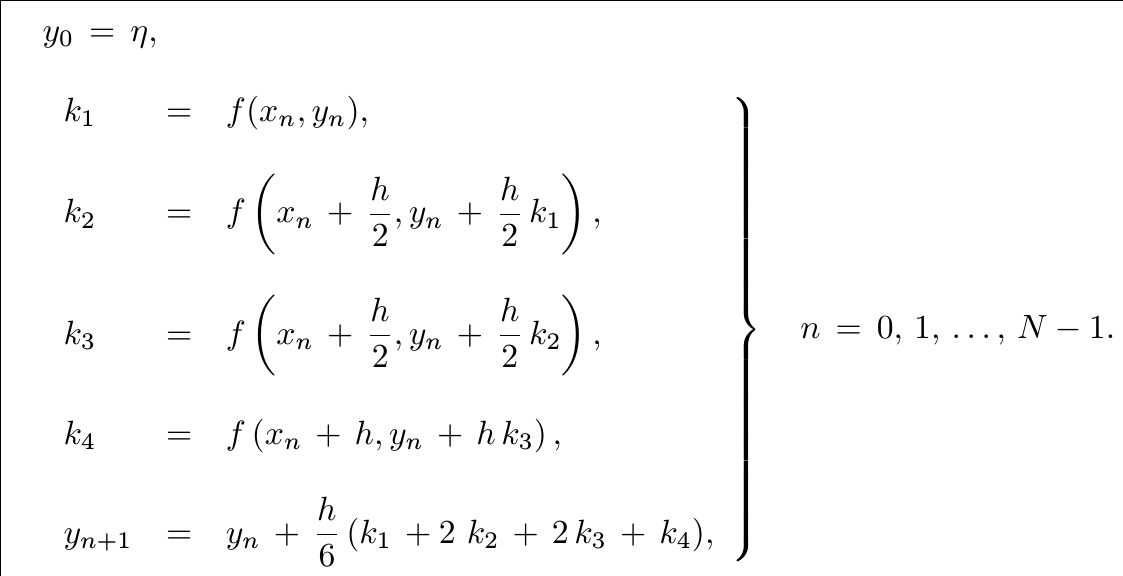
\includegraphics[width=0.9\linewidth]{tema4/R-K-clasico}
  \end{center}
\end{example}

\section{Métodos multipaso}
\label{sec:metodos-multipaso}

Los métodos numéricos de $k$ son aquellos en los que, para calcular
$y_{n+k}$ (una aproximación de $\sol(t_{n+k})$), se utilizan
aproximaciones de la solución en $k$ etapas de tiempo anteriores,
\begin{equation*}
  y_n,\  y_{n+1},\ \dots, y_{n+k-1} \quad \longmapsto \quad y_{n+k}.
\end{equation*}
Específicamente:
\begin{definition}
  Un método numérico (lineal) de $k$ pasos para aproximar la solución
  de~(\ref{eq:pvi}) es todo aquel en el que la solución en
  la etapa $n+k$ viene dada por una expresión recursiva de la forma:
  \begin{align}
    \label{eq:metodo-multipaso}
    \ddt y_{n+k}=&\sum_{j=0}^k \beta_j f(t_{n+j},y_{n+j}), \quad
    n=0,\dots,N-k, \intertext{donde $\ddt y_{n+k}$ es un aproximación
      de $\sol'(t_{n+k})$ usando un cociente incremental con $k$ pasos:}
    \ddt
    \label{eq:cociente-incremental-multipaso}
    y_{n+k}&=\frac{1}{h}\sum_{j=0}^k\alpha_j y_{n+j}.
  \end{align}
\end{definition}
En las expresiones anteriores, $\alpha_j, \beta_j\in\Rset$, con
$\alpha_k\neq 0$. Por simplificar, supondremos $$\alpha_k=1$$ (lo que
equivale a dividir todos los coeficientes por $\alpha_k$).

Por ejemplo, los métodos de Euler (explícito e implícito) y el esquema
de Crank-Nicolson~(\ref{eq:crank-nicolson-2}) son métodos de este tipo
con un único paso $k=1$. Más adelante se muestran algunos métodos con
$k>1$.
Con el fin de abreviar, con frecuencia usaremos la siguiente notación:
$$f_n=f(\tn,\yn).$$

Puesto que en un método de $k$ pasos del
tipo~(\ref{eq:metodo-multipaso}) se necesitan $k$ aproximaciones
previas para calcular $y_{n+k}$, en la primera iteración ($n=0$) es
necesario disponer de $k$ valores de arranque, $y_0$, $y_1$, \dots,
$y_{k-1}$ (que determinarán $y_k$). Pero en~(\ref{eq:pvi}) sólo
contamos con un dato inicial, $\ycero$, de forma que necesitaremos
usar algún método numérico para aproximar $y_1$, $y_2$, \dots,
$y_{k-1}$. Habitualmente se usarán métodos de un paso, con especial
cuidado en que el orden de estos métodos sea (al menos) igual al
del método multipaso (pues, de otra forma, perderíamos calidad en la
aproximación inicial).

\begin{enumerate}
\item Si $\beta_k=0$, el método se dice \emph{explícito}. El término
  $f_{n+k}=f(t_{n+k},y_{n+k})$ no aparece en el segundo miembro
  de~(\ref{eq:metodo-multipaso}) del método multipaso, en
  consecuencia, usando~(\ref{eq:cociente-incremental-multipaso}),
  $y_{n+k}$ puede expresarse explícitamente:
  \begin{equation*}
    y_{n+k}=
    h\sum_{j=0}^{k-1} \beta_j f_{n+j}-\sum_{j=0}^{k-1}\alpha_j y_{n+j}.
  \end{equation*}
\item Si $\beta_k\neq 0$, el método se dice \emph{implícito}. No podemos
  expresar explícitamente el término $y_{n+k}$ y, en cada paso,
  para calcular este término será necesario resolver la ecuación (no
  lineal, en general):
  \begin{equation*}
    y_{n+k} - \beta_k f(t_{n+j},y_{n+j})=
     h\sum_{j=0}^{k-1} \beta_j f(t_{n+j},y_{n+j})- \sum_{j=0}^{k-1}\alpha_j y_{n+j} .
  \end{equation*}
  Para resolver este tipo de ecuaciones existen distintas
  posibilidades, las más habituales de las cuales son el método de
  aproximaciones sucesivas (o de punto fijo) y el método de Newton
  (para asegurar la convergencia, de estos métodos, será necesario
  imponer hipótesis adicionales a $f$).
\end{enumerate}

\subsection*{Construcción de métodos multipaso lineales}

Para deducir algunos métodos multipaso utilizaremos la formulación
integral de la ecuación diferencial
$$
y'=f(t,y),
$$
es decir fijados $t,t^*\in[a,b]$ escribimos
\begin{equation*}
  \sol(t^*)-\sol(t) = \int_{t}^{t^*} f(x,\sol(x))\, dx.
\end{equation*}
Para cada $n=0,\dots,N-k$, elegimos $t=x_{n+k-1}$ y $t^*=x_{n+k}$ y
denotando $y_{n+j}\approx \sol(t_{n+j})$ a las aproximaciones que
deseamos calcular,  ponemos en práctica la siguiente idea:
  % realizar, en esta formulación integral las siguiente
% aproximación:
\begin{enumerate}
\item Elegir $t=x_{n+k-1}$ y $t^*=x_{n+k}$
% \item Elegir $t$ y $t^*$ adecuadamente.
% \item Sustituir la función $F(t)=f(t,\sol(t))$ por su polinomio de
%   interpolación de Lagrange, $P(t)$, en los nodos $t_n,\ t_{n+1},\
%   \dots, t_{n+k}$.
\item Sustituir la función $F(x)=f(x,\sol(x))$ por su polinomio de
  interpolación de Lagrange, $P(x)$, en un soporte
  $S\subset \{t_{n+j}\}_{j=0}^k$ adecuado:%  interpola los valores
  % $\{f(t_{n+j},y_{n+j})\}_{j=0}^k$.
  \begin{enumerate}
  \item Métodos de \emph{\AB}:
    \begin{equation*}
      S= \{t_{n+j}\}_{j=0}^{k-1}.
    \end{equation*}
    Como veremos, se trata de métodos explícitos, pues en la
    aproximación no aparece el término
    $f(t_{n+k},y_{n+k})$.
  \item  Métodos de \emph{\AM}:
    \begin{equation*}
      S= \{t_{n+j}\}_{j=0}^{k},
    \end{equation*}
    dando lugar a métodos implícitos.
  \end{enumerate}
\end{enumerate}

\begin{example}[Método de \AB de dos pasos (orden 2)]
  \label{sec:AB-dos-pasos}
  Consideremos la siguiente expresión integral:
  \begin{equation}
   \label{eq:tema4:8}
   \sol(t_{n+2})-\sol(t_{n+1}) \approx \int_{t_{n+1}}^{t_{n+2}} P(t)\,dt,
  \end{equation}
  donde $P(t)$ es el polinomio de interpolación de $F(t)=f(t,\sol(t))$ en
  $t_n$ y $t_{n+1}$. Para construirlo, podemos usar la fórmula de
  diferencias dividas de Newton o bien la fórmula de Lagrange. En este
  último caso:
  \begin{equation*}
   P(t)=F(t_n)\frac{t-t_{n+1}}{t_n-t_{n+1}} +
   F(t_{n+1})\frac{t-t_{n}}{t_{n+1}-t_{n}}.
  \end{equation*}
  Con un simple cálculo (puede ser útil el cambio de variable $t =
  t_{n+1}+h\,s$, que transforma $t\in [t_{n+1},t_{n+2}]$ en $s\in [0,1]$)
  el segundo miembro de~(\ref{eq:tema4:8}) resulta:
  \begin{equation*}
  \int_{t_{n+1}}^{t_{n+2}} P(t)\,dt = \frac{h}{2} \big[
  3(f(t_{n+1},\sol(t_{n+1})) - f(t_{n},\sol(t_{n})) \big].
  \end{equation*}
  Planteamos, por tanto, la siguiente aproximación: dados $y_n$,
  $y_{n+1}$, calcular $y_{n+2}$ como solución de la
  siguiente fórmula de recurrencia:
  \begin{equation}
    \tag{AB2}
    \label{eq:AB2}
    y_{n+2}-y_{n+1} = \frac{h}{2} \big[
    3f(t_{n+1},y_{n+1}) - f(t_{n},y_{n}) \big],
  \end{equation}
  de donde, para cada $n=0,\dots,N-2$ podemos obtener explícitamente el
  valor $y_{n+2}$.

  El valor $y_0$ se puede obtener a partir del dato inicial $\ycero$,
  mientras que para el cálculo de $y_1$ será necesario utilizar un
  método numérico de un paso. Se puede demostrar que este método
  de \AB tiene orden 2, por tanto el método para inicializar debe
  tener el mismo orden (por ejemplo, Euler--Cauchy o Euler mejorado).
\end{example}

\begin{example}[Método de \AM de dos pasos (orden 2)]
  Si consideramos la ecuación integral (\ref{eq:tema4:8}) pero
  definimos $P(t)$ como el polinomio de interpolación de
  $f(t,\sol(t))$ en $\{t_n,t_{n+1},t_{n+2}\}$, obtenemos el método
  de \AM de dos pasos. Procediendo como en el ejemplo anterior (lo que
  se deja como ejercicio) se obtiene:
  \begin{equation}
    \tag{AM2}
    \label{eq:AM2}
      y_{n+2}-y_{n+1} = \frac{h}{12} \big[
      5f(t_{n+2},y_{n+2}) + 8 f(t_{n+1},y_{n+1}) - f(t_{n},y_{n}) \big].
  \end{equation}
  Se puede demostrar que el orden de este método es igual a
  $2$. Puesto que se trata de un método implícito, en principio será
  necesario usar algún método numérico (por ejemplo, iteraciones de
  punto fijo) en cada instante $\tn$ para hallar $y_{n+2}$.
\end{example}

\begin{example}[Método predictor-corrector~(\ref{eq:AB2})--(\ref{eq:AM2})]
  Con frecuencia, los métodos de \AB y \AM del mismo orden se suelen
  combinar para dar lugar a nuevos métodos numéricos. La idea es, en
  cada etapa $t_n$:
  \begin{enumerate}
  \item Utilizar el método de \AB para obtener, de forma explícita una
    primera aproximación (predicción) de $y_{n+k}$.
  \item Utilizar la predicción obtenida para aproximar
    $f(t_{n+k},y_{n+k})$ y así calcular, mediante el método de \AM,
    una nueva aproximación (corrección) de $y_{n+k}$.
  \end{enumerate}

  En el caso~(\ref{eq:AB2})--(\ref{eq:AM2}) cada etapa del método
  queda:
  \begin{equation*}\left\{
      \begin{aligned}
        y^*_{n+2} &= y_{n+1} + \frac{h}{2} \big[ 3f(t_{n+1},y_{n+1}) -
        f(t_{n},y_{n}) \big] \quad \text{(predicción),}
        \\
        y_{n+2} &= y_{n+1} + \frac{h}{12} \big[ 5f(t_{n+2},y^*_{n+2})
        + 8 f(t_{n+1},y_{n+1}) - f(t_{n},y_{n}) \big] \quad
        \text{(corrección).}
      \end{aligned}\right.
  \end{equation*}
  Así obtenemos un método explícito que saca partida a las
  características de los esquemas de \AB y AM.
  \end{example}

%%% Local Variables:
%%% mode: latex
%%% TeX-master: "../tema4.tex"
%%% End:


\end{document}

%%% Local Variables:
%%% mode: latex
%%% TeX-master: t
%%% End:
